%%%%%%%%%%%%%%%%%%%%%%%%%%%%%%%%%%%%%%%%%
% Masters/Doctoral Thesis 
% LaTeX Template
% Version 1.43 (17/5/14)
%
% This template has been downloaded from:
% http://www.LaTeXTemplates.com
%
% Original authors:
% Steven Gunn 
% http://users.ecs.soton.ac.uk/srg/softwaretools/document/templates/
% and
% Sunil Patel
% http://www.sunilpatel.co.uk/thesis-template/
%
% License:
% CC BY-NC-SA 3.0 (http://creativecommons.org/licenses/by-nc-sa/3.0/)
%
% Note:
% Make sure to edit document variables in the Thesis.cls file
%
%
% Modified and Adapted by Michael Lees 2020
%%%%%%%%%%%%%%%%%%%%%%%%%%%%%%%%%%%%%%%%%

%----------------------------------------------------------------------------------------
%	PACKAGES AND OTHER DOCUMENT CONFIGURATIONS
%----------------------------------------------------------------------------------------

\documentclass[11pt, oneside]{Thesis} % The default font size and one-sided printing (no margin offsets)

% \graphicspath{{Pictures/}} % Specifies the directory where pictures are stored

\usepackage[square, numbers, comma, sort&compress]{natbib} % Use the natbib reference package - read up on this to edit the reference style; if you want text (e.g. Smith et al., 2012) for the in-text references (instead of numbers), remove 'numbers' 
\usepackage[ruled,vlined]{algorithm2e}
\usepackage{amsmath}
\usepackage{booktabs}

\usepackage[utf8]{inputenc}
% \usepackage{amsmath}
\usepackage{bm}
\usepackage[normalem]{ulem}
% \usepackage{todonotes}
\usepackage{amssymb}
% \usepackage[colorlinks]{hyperref}
\usepackage[symbols,nogroupskip,sort=none]{glossaries-extra}
\usepackage{makecell}
% \usepackage{minted}
\usepackage[singlelinecheck=false,font=small,labelfont=bf]{caption}
\usepackage{wrapfig}
\usepackage{listings}
\usepackage{xcolor}
\usepackage{multirow}
\usepackage{subcaption}
\usepackage[T1]{fontenc}
\usepackage{lstbayes}

\usepackage{titlesec, blindtext, color}
\definecolor{gray75}{gray}{0.75}
\newcommand{\hsp}{\hspace{20pt}}

\titleformat{\chapter}[hang]{\Huge\bfseries}{\thechapter\hsp\textcolor{gray75}{|}\hsp}{0pt}{\Huge\bfseries}


\definecolor{codegreen}{rgb}{0,0.6,0}
\definecolor{codegray}{rgb}{0.5,0.5,0.5}
\definecolor{codepurple}{rgb}{0.58,0,0.82}
\definecolor{backcolour}{rgb}{0.95,0.95,0.92}

\lstdefinestyle{mystyle}{
    backgroundcolor=\color{backcolour},   
    commentstyle=\color{codegreen},
    keywordstyle=\color{magenta},
    numberstyle=\tiny\color{codegray},
    stringstyle=\color{codepurple},
    basicstyle=\ttfamily\footnotesize,
    breakatwhitespace=false,         
    breaklines=true,                 
    captionpos=b,                    
    keepspaces=true,                 
    numbers=left,                    
    numbersep=5pt,                  
    showspaces=false,                
    showstringspaces=false,
    showtabs=false,                  
    tabsize=2
}

\lstset{style=mystyle}

% \usepackage[demo]{graphicx}
\captionsetup[table]{singlelinecheck=off}

\DeclareMathOperator*{\argmin}{arg\,min}
\DeclareMathOperator*{\argmax}{arg\,max}
\hypersetup{urlcolor=blue, colorlinks=true} % Colors hyperlinks in blue - change to black if annoying
\title{\ttitle} % Defines the thesis title - don't touch this

\begin{document}

\frontmatter % Use roman page numbering style (i, ii, iii, iv...) for the pre-content pages
\setstretch{1.3} % Line spacing of 1.3

% Define the page headers using the FancyHdr package and set up for one-sided printing
\fancyhead{} % Clears all page headers and footers
\rhead{\thepage} % Sets the right side header to show the page number
\lhead{} % Clears the left side page header

\pagestyle{fancy} % Finally, use the "fancy" page style to implement the FancyHdr headers

\newcommand{\HRule}{\rule{\linewidth}{0.5mm}} % New command to make the lines in the title page

% PDF meta-data
\hypersetup{pdftitle={\ttitle}}
\hypersetup{pdfsubject=\subjectname}
\hypersetup{pdfauthor=\authornames}
\hypersetup{pdfkeywords=\keywordnames}

%----------------------------------------------------------------------------------------
%	TITLE PAGE
%----------------------------------------------------------------------------------------

\begin{titlepage}
\begin{center}

\textsc{\LARGE \univname}\\[1.5cm] % University name
\textsc{\Large Masters Thesis}\\[0.5cm] % Thesis type

\HRule \\[0.4cm] % Horizontal line
{\huge \bfseries \ttitle}\\[0.4cm] % Thesis title
\HRule \\[1.5cm] % Horizontal line
 
\begin{minipage}{0.4\textwidth}
\begin{flushleft} \large
\emph{Author:}\\
\href{http://yourwebaddress.com}{\authornames} % Author name - remove the \href bracket to remove the link
\end{flushleft}
\end{minipage}
\begin{minipage}{0.4\textwidth}
\begin{flushright} \large
\emph{Supervisor:} \\
\href{http://mhlees.com}{\supname} % Supervisor name - remove the \href bracket to remove the link  
\end{flushright}
\end{minipage}\\[3cm]
 
\large \textit{A thesis submitted in partial fulfilment of the requirements\\ for the degree of \degreename}\\[0.3cm] % University requirement text
\textit{in the}\\[0.4cm]
\groupname\\\deptname\\[2cm] % Research group name and department name
 
{\large \today}\\[2cm] % Date

\includegraphics[width=0.6\textwidth]{clslogo.png} % Include Computational Science Logo
 
\vfill
\end{center}

\end{titlepage}

%----------------------------------------------------------------------------------------
%	DECLARATION PAGE
%	Your institution may give you a different text to place here
%----------------------------------------------------------------------------------------

\Declaration{

\addtocontents{toc}{\vspace{1em}} % Add a gap in the Contents, for aesthetics

I, \authornames, declare that this thesis, entitled `\ttitle' and the work presented in it are my own. I confirm that:

\begin{itemize} 
\item[\tiny{$\blacksquare$}] This work was done wholly or mainly while in candidature for a research degree at the University of Amsterdam.
\item[\tiny{$\blacksquare$}] Where any part of this thesis has previously been submitted for a degree or any other qualification at this University or any other institution, this has been clearly stated.
\item[\tiny{$\blacksquare$}] Where I have consulted the published work of others, this is always clearly attributed.
\item[\tiny{$\blacksquare$}] Where I have quoted from the work of others, the source is always given. With the exception of such quotations, this thesis is entirely my own work.
\item[\tiny{$\blacksquare$}] I have acknowledged all main sources of help.
\item[\tiny{$\blacksquare$}] Where the thesis is based on work done by myself jointly with others, I have made clear exactly what was done by others and what I have contributed myself.\\
\end{itemize}


% Signed: \\\\\includegraphics[width=3cm]{Pictures/yoursignature.pdf} \\
%\rule[1em]{25em}{0.5pt} % This prints a line for the signature
 
Date: 10 July 2020\\
%\rule[1em]{25em}{0.5pt} % This prints a line to write the date
}

\clearpage % Start a new page

%----------------------------------------------------------------------------------------
%	QUOTATION PAGE
%----------------------------------------------------------------------------------------

\pagestyle{empty} % No headers or footers for the following pages

\null\vfill % Add some space to move the quote down the page a bit

\textit{``Statistics is the grammar of science."}

\begin{flushright}
Karl Pearson
\end{flushright}

\vfill\vfill\vfill\vfill\vfill\vfill\null % Add some space at the bottom to position the quote just right

\clearpage % Start a new page

%----------------------------------------------------------------------------------------
%	ABSTRACT PAGE
%----------------------------------------------------------------------------------------

\addtotoc{Abstract} % Add the "Abstract" page entry to the Contents

\abstract{\addtocontents{toc}{\vspace{1em}} % Add a gap in the Contents, for aesthetics
% Include your abstract here 
% Abstracts must include sufficient information for reviewers to judge the nature and significance
% of the topic, the adequacy of the investigative strategy, the nature of the results, and the
% conclusions. The abstract should summarize the substantive results of the work and not merely
% list topics to be discussed. 
% Length 200-400 words.
Single cell RNA sequencing (scRNA-seq) has progressed the biological sciences by allowing researchers to obtain a rough estimate of the number of transcripts in a cell for every gene. Modern advancements in the field of scRNA-seq have enabled the reading of thousands of genes in thousands to even millions of cells. Techniques like scRNA-seq therefore return high dimensional data-sets, which are hard to visualize in only two dimensions. The analysis and visualization of such data have been performed by linear (PCA, PPCA) and later non-linear (t-SNE, UMAP) dimensionality reduction techniques. In this report, we examine the role of hierarchical mixtures of probabilistic PCAs (HmPPCAs) for the visualization of scRNA-seq data. At the same time, we explore the use of probabilistic programming to define and solve probabilistic models easily, without the need to derive the necessary equations to solve them manually.

The HmPPCAs model was implemented in the probabilistic programming language Stan and evaluated on 2 scRNA-seq data-sets from the literature and 5 simulated data-sets of various dimensionalities. The model is solved using NUTS (an extension to Hamiltonian Monte Carlo) and ADVI (an extension to variational inference) to get a better grasp of two different methods used in probabilistic programming. We then compared the HmPPCAs results with results obtained using other popular techniques like t-SNE and UMAP. The plots obtained through all methods were tested for their cell type separability.

The results show that ADVI provides statistical modellers with a fast way to approach solutions without sacrificing much of the performance. Although HmPPCAs did not achieve the same visualization performance as UMAP and t-SNE, the results show that extending linear dimensionality reduction techniques with hierarchy can show structures that are not noticeable when using a single non-hierarchical dimensionality reduction.
% Where a PPCA shows clusters within the whole data-set, the addition of hierarchy reveals structures within those clusters that would otherwise not have been noticeable.
}

\clearpage % Start a new page

%----------------------------------------------------------------------------------------
%	ACKNOWLEDGEMENTS
%----------------------------------------------------------------------------------------

\setstretch{1.3} % Reset the line-spacing to 1.3 for body text (if it has changed)

\acknowledgements{\addtocontents{toc}{\vspace{1em}} % Add a gap in the Contents, for aesthetics

% Thank the people that have helped, supervisors family etc.
% \todo{do cool thing with this}
% I wish to acknowledge that black lives matter.
% Joel, Ivander, Mama, Perry zoieso,  Ruby?, Ismay?, Emma???? Anna?,  Roberto?
I want to thank Perry for helping and understanding and dedicating so much of his time to me and this project.

I also thank Joel, for guiding me through all the negatives, and I thank Ivander for bringing all the positives. I love these people!

I thank the people who helped me for making my life easier and I thank the difficult moments in my life for teaching me how to grow.

I feel very grateful towards the plants and trees on this planet, some of which who were the best listeners and who always seemed to know the right thing to do.
% I also thank Joel, for helping me with the negatives and .
% And I thank Ivander for bringing the positives! I love these people!

I thank my mom, for listening, talking and being cool!

And I thank the universe for giving birth to this all!
}
\clearpage % Start a new page

%----------------------------------------------------------------------------------------
%	LIST OF CONTENTS/FIGURES/TABLES PAGES
%----------------------------------------------------------------------------------------

\pagestyle{fancy} % The page style headers have been "empty" all this time, now use the "fancy" headers as defined before to bring them back

\lhead{\emph{Contents}} % Set the left side page header to "Contents"
\tableofcontents % Write out the Table of Contents

\lhead{\emph{List of Figures}} % Set the left side page header to "List of Figures"
\listoffigures % Write out the List of Figures

\lhead{\emph{List of Tables}} % Set the left side page header to "List of Tables"
\listoftables % Write out the List of Tables

\lhead{\emph{List of Algorithms}} % Set the left side page header to "List of Algorithms"
\addtotoc{List of Algorithms}
\listofalgorithms % Write out the List of Tables

%----------------------------------------------------------------------------------------
%	ABBREVIATIONS
%----------------------------------------------------------------------------------------

\clearpage % Start a new page

\setstretch{1.5} % Set the line spacing to 1.5, this makes the following tables easier to read

\lhead{\emph{Abbreviations}} % Set the left side page header to "Abbreviations"
\listofsymbols{ll} % Include a list of Abbreviations (a table of two columns)
{
\textbf{ADVI} & \textbf{A}utomatic \textbf{D}ifferentiation \textbf{V}ariational \textbf{I}nference\\
\textbf{BIC} & \textbf{B}ayesian \textbf{I}nformation \textbf{C}riterion\\
\textbf{CSL} & \textbf{C}omputational \textbf{S}cience \textbf{L}ab\\
\textbf{ELBO} & \textbf{E}vidence \textbf{L}ower \textbf{BO}und\\
\textbf{EM} & \textbf{E}xpectation-\textbf{M}aximization\\
\textbf{GMM} & \textbf{G}aussian \textbf{M}ixture \textbf{M}odel\\
\textbf{HMC} & \textbf{H}amiltonian \textbf{M}onte \textbf{C}arlo\\
\textbf{HmPPCAs} & \textbf{H}ierarchical \textbf{M}o\textbf{PPCAs}\\
\textbf{HSPC} & \textbf{h}ematopoietic \textbf{s}tem and \textbf{p}rogenitor \textbf{c}ells\\
\textbf{LT\_SHC} & \textbf{l}ong-\textbf{t}erm \textbf{h}ematopoietic \textbf{s}tem \textbf{c}ells\\
\textbf{MC} & \textbf{M}onte \textbf{C}arlo\\
\textbf{ML} & \textbf{M}aximum \textbf{L}ikelihood\\
\textbf{MoPPCAs} & \textbf{M}ixture \textbf{o}f \textbf{PPCAs}\\
\textbf{NUTS} & \textbf{N}o \textbf{U}-\textbf{T}urn \textbf{S}ampler\\
\textbf{PCA} & \textbf{P}rincipal \textbf{C}omponent \textbf{A}nalysis\\
\textbf{PPCA} & \textbf{P}robabilistic \textbf{PCA}\\
\textbf{scRNA-seq} & \textbf{S}ingle \textbf{C}ell \textbf{RNA S}equencing\\
\textbf{t-SNE} & \textbf{t}-\textbf{D}istributed \textbf{S}tochastic \textbf{N}eighbour \textbf{E}mbedding\\
\textbf{UMAP} & \textbf{U}niform \textbf{M}anifold \textbf{A}pproximation and \textbf{P}rojection\\
\textbf{UvA} & \textbf{U}niversiteit \textbf{v}an \textbf{A}msterdam\\
\textbf{VB} & \textbf{V}ariational \textbf{B}ayes\\
\textbf{VI} & \textbf{V}ariational \textbf{I}nference\\


% \textbf{Acronym} & \textbf{W}hat (it) \textbf{S}tands \textbf{F}or \\
}

%----------------------------------------------------------------------------------------
%	PHYSICAL CONSTANTS/OTHER DEFINITIONS
%----------------------------------------------------------------------------------------

% \clearpage % Start a new page

% \lhead{\emph{Physical Constants}} % Set the left side page header to "Physical Constants"

% \listofconstants{lrcl} % Include a list of Physical Constants (a four column table)


%{
%Speed of Light & $c$ & $=$ & $2.997\ 924\ 58\times10^{8}\ \mbox{ms}^{-\mbox{s}}$ (exact)\\
%% Constant Name & Symbol & = & Constant Value (with units) \\
%}

%----------------------------------------------------------------------------------------
%	SYMBOLS
%----------------------------------------------------------------------------------------

\clearpage % Start a new page

\lhead{\emph{Symbols}} % Set the left side page header to "Symbols"

% \printunsrtglossary[type=symbols,style=long]

\listofnomenclature{lll} % Include a list of Symbols (a three column table)
{

$\bm{x}$ & $d$-dimensional observed data-point\\
$\bm{X}$ & $n\times d$ matrix describing the observed data-set\\
$\bm{z}$ & $m$-dimensional latent data-point\\
$\bm{Z}$ & $n\times m$ matrix describing the latent data-set\\
$\bm{\mu}$ & $d$-Dimensional mean of $\bm{x}$\\
$\sigma$ & Standard deviation of $\bm{x}$\\
$\bm{\Sigma}$ & Covariance matrix of $\bm{X}$\\
$n$ & Number of data-points in data-set\\
$d$ & Number of dimensions of one variable\\
$K$ & Number of mixture components\\
$\pi_k$ & Mixture coefficients\\



% $a$ & distance & m \\
% $P$ & power & W (Js$^{-1}$) \\
% Symbol & Name & Unit \\

% & & \\ % Gap to separate the Roman symbols from the Greek

% $\omega$ & angular frequency & rads$^{-1}$ \\
% Symbol & Name & Unit \\
}

%----------------------------------------------------------------------------------------
%	DEDICATION
%----------------------------------------------------------------------------------------

\setstretch{1.3} % Return the line spacing back to 1.3

\pagestyle{empty} % Page style needs to be empty for this page

\addtocontents{toc}{\vspace{2em}} % Add a gap in the Contents, for aesthetics

%----------------------------------------------------------------------------------------
%	THESIS CONTENT - CHAPTERS
%----------------------------------------------------------------------------------------

\mainmatter % Begin numeric (1,2,3...) page numbering

\pagestyle{fancy} % Return the page headers back to the "fancy" style
% \pagestyle{thesis}
% Include the chapters of the thesis as separate  tex files from the Chapters folder
% Change the file names if you prefer

%This structure provides a bare bones essentials of the thesis and some indicative length
%This structure may not fit your thesis perfectly, but be sure to include these components somehow.
%It is possible to split the chapters up (E.g., 2 methods chapter, Experiment and Results as two, etc.)

% The typical length may be between 43 - 64 pages. Do not worry if you go slightly larger or smaller than this. 
% But a thesis of 20 pages, or 100 pages may suggest you've been to brief or too verobse.
%NOTE - there is not strict limit/minimum.


% \chapter{Introduction}
\lhead{\emph{Introduction}}
% \subsection{Gene-expression analysis and dimensionality reduction}
% \subsubsection{Gene-expression}
Gene expression is the process where genes on the DNA are transcribed and used to create specific products. It is the process that sets the synthesis of proteins from the DNA in motion and it is fundamental to all biological mechanisms. When a gene is expressed, its DNA sequence is copied to a piece of mRNA, which can then be translated into a protein. Genes that are highly expressed are being transcribed to mRNA more often than genes that are lowly expressed, so the number of mRNA transcripts for these genes is relatively high. Given the biological and medical significance of this process, it is studied broadly and techniques for quantitative measurement have been developed over the last decades.
RNA sequencing (\textbf{RNA-seq}) measures the relative level of expression of genes by quantifying the number of mRNA transcripts. This approach measures the average levels of gene expression across a population of cells, which possibly consists of different cell types. This is a limitation to many experiments because results are not specific to one individual cell.
Single-cell RNA-sequencing (scRNA-seq) \cite{haque2017practical} has given the means to analyse the expression patterns of large numbers of genes from specifically chosen cells. 
First, a sample of specifically chosen cells is collected. The cells undergo a lysis step that permeates their membrane but leaves the RNA intact. The mRNA is then reverse-transcribed to its complementary cDNA. The newly acquired cDNA is amplified, through polymerase chain reaction (PCR) or in vitro amplification. Finally, this cDNA is sequenced and the resulting sequence reads are mapped back to the genome, pieces of cDNA that match with a gene are counted.

This technique has seen a rise in popularity \cite{shapiro2013single}. ScRNA-seq was first pioneered in the late 2000's \cite{tang2009mrna}. %\cite{weber2015discovering, nagalakshmi2008transcriptional}. 
The new invention of scRNA-seq allowed researchers to study individual cell types and to compare different cell types. For example, cells from different embryonic stages might be compared to study the activity of genes during embryonic development \cite{deng2014single}. Another example would be the detection of malignant tumor cells in otherwise healthy cell populations \cite{tirosh2016dissecting}.


%When RNA-seq first started out, the RNA of one cell from one species was analyzed. This allowed the observers to write evaluations on the transcriptome of one species. Since then, the technology has evolved enough to allow the analysis of the transcriptome of thousands of cells. One advantage of this is that, now, multiple groups of different cells can be studied and compared. For example, it is possible to compare cells from different body parts or in different health conditions. Newer technologies have even been invented to enable the comparison of different species, despite their different genomes \cite{aubry2014deep}. However, comparing multiple groups of cells did require new forms of analysis. Seeing as how samples contain the expression levels of a large number of genes, it may be tedious to compare each and every of those genes for different groups. Moreover, it is hard to summarize the findings on one of such an experiment into one visualization plot that represents most or all of the information obtained through the experiment. 

% \subsubsection{Dimensionality reduction for visualization purposes}
For the comparison of transcriptomes of different cell types, it is often desirable to visualize the gene expression levels of individual cells in a simple yet informative way.
It may not be hard to visualize data in two dimensions, for instance, one could generate a scatter-plot of two genes, where each point corresponds to one cell. Simple correlations should then easily become visible. For three dimensions or genes, a 3D plot can be generated similarly. For data of more dimensions, it is possible to produce multiple plots for every combination of two dimensions. However, scRNA-seq deals with data that may exceed thousands of genes, which is hard to visualize in a way that preserves most information. Dimensionality reduction has therefore become an important topic in scRNA-seq data analysis. Techniques like principal component analysis (\textbf{PCA}) \cite{pearson1901liii}, probabilistic PCA (\textbf{PPCA}) \cite{ppca}, t-distributed stochastic neighbour embedding (\textbf{t-SNE}) \cite{maaten2008visualizing} and uniform manifold approximation and projection (\textbf{UMAP}) \cite{mcinnes2018umap, becht2019dimensionality} (among others) deal with dimensionality reduction and try to transform high-dimensional data to 2 or 3 dimensional data in the most adequate ways. For instance, PCA projects the data onto lesser dimensions, known as the principal components, in such a manner that the variance of the projected data is kept at a maximum. PPCA attempts to find latent random variables that explain the observed data in a probabilistic way. These techniques are linear. T-SNE and UMAP are non-linear techniques. These techniques put the data-points in the low dimensional space by specifying an attractive force between points that are closely related in the data space and a repellent force between other points.

Another way to induce non-linearity is by adding hierarchical layers. For example, a hierarchical mixture of PPCAs (\textbf{HmPPCAs}) \cite{bishop1998hierarchical} is able to divide the data into different clusters and returns their individual low-dimensional representation. It has been argued that each of these clusters might have different optimal representations in the low-dimensional space. While one cluster can be best described by two principal components, another cluster might be better represented by two different principal components. Representing every cluster by the same principal components might be optimal for the whole data-set, but not for the separate clusters. This model has been used for the analysis of scRNA-seq data \cite{philipsthesis}. However, this model was introduced as an interactive model, which still requires the user to select the number of different clusters and their approximate locations in the low-dimensional space. User input may be susceptible to human subjectivity and inconsistency. It also requires the user to wait for the parameter estimation to finish so that they can initiate the next level. Here, we develop a model that works in a fully automated way and does not require extra user-input.

Another difference to our model is how it is solved. Some of the mentioned techniques, like PCA and PPCA, have a closed-form solution. Alternatively, it is possible to use an Expectation-Maximization (\textbf{EM}) algorithm (see Appendix \ref{app:gmm_em}), which is guaranteed to converge to a local optimum, with lower computational cost than the closed-form solution. The HmPPCAs model as proposed originally was solved using an EM-algorithm as well \cite{bishop1998hierarchical, philipsthesis}. However, another approach to find a solution to the HmPPCAs is through probabilistic programming. Probabilistic programming entails programming a probabilistic model and having the underlying distributions of the parameters found automatically. Platforms for statistical optimization, like TensorFlow Probability \cite{dillon2017tensorflow} and Stan \cite{carpenter2017stan} have been released as an alternative way to approach solutions to statistical problems. These are Bayesian probabilistic programming languages. Using tools like these has the benefit that the user can specify and manipulate statistical models without having to derive and solve the necessary equations. This increases the range of models to be studied and enables the user to easily refine parts of the model without having to rewrite the entire solution. These tools do not only give the users a solution to their model, but they can also give more information about the solution as they compute (an approximation of) the entire probability function of the parameters of the model given the input data. The models created in this report will be created within the Stan environment using Python as the primary programming language. Stan is able to automate the inference of probabilistic models in two ways. The first is by sampling through the No U-Turn Sampler (\textbf{NUTS}), which is an extension to the Hamiltonian Monte Carlo method. The other is an algorithm called automatic differentiation variational inference (\textbf{ADVI}). Both these methods will be discussed in Section \ref{sec:stan}

% Models like these have been the status quo for scRNA-seq visualization and a variety of other purposes. But even though these models hold large value to gene-expression analysis, they are not tuned specifically for this function. More recently, some models have been developed that are tailored specifically for gene-expression analysis  \cite{zifa}. Next to that, many of those models are expanded to find more and more complex structures in data generally  \cite{bishop2002bayesian}, which could also qualitatively improve expression-pattern analysis. The objective of these writings is to produce a dimensionality reduction model, suited specifically for the purpose of gene-expression data.

% To achieve this, we will attempt to incorporate a range of technical developments in the field to the existing PPCA model.\todo{whats new in this model? difference from hmppca} The model can then be compared with other models\todo{which models?} 

Since we will mainly extend the HmPPCAs model, Section \ref{sec:approach} starts with the theory behind PPCA and hmPPCAs models. We then continue by discussing Stan and the sampling methods used to solve our models. We then conclude this section with a description of the algorithm used for this project. Section \ref{sec:methods} describes the setup of the model and the experiments to evaluate our model and to compare it with other models. The results of these experiments will be discussed in Section \ref{sec:results}, and we conclude this report with a brief discussion in Section \ref{sec:discussion}. %Set out your thesis and state your research question (5-8 pages)
% \input{Chapters/LiteratureReview} %Related literature and material (8-12 pages)
% \chapter{Methods}\label{sec:methods}
\lhead{\emph{Methods}}

\section{Data description}\label{sec:data}
Two types of data-sets were used. The first type consisted of simulated data-sets generated using Splatter \cite{zappia2017splatter}. This is an R-package that allows the user to generate customized scRNA-seq data-sets. Since Splatter data-sets are easily obtainable and customizable, two different types of data-sets were generated: one simple type which contained five groups of cells that were easy to differentiate from each other and one complex type containing six groups of cells which showed more overlap in their patterns. The difference in complexity of these data-sets was regulated by use of the `de.facLoc', `de.facScale' and the `de.prob' parameters. These parameters describe how easily diffent groups can be separated. The last parameter `de.prob', the probability with which genes in a group were differentially expressed, was set higher for the complex data-sets than for the simple data-sets, as the different groups of cell-types were not distinguishable without doing so. For the simple Splatter data-sets, de.prob was set higher for the data-sets containing fewer genes, to make sure that each data-set contained enough differentially expressed genes. For the complex Splatter data-sets, this was not necessary, as de.prob was high enough already for even the data-set containing 5 genes. For both the simple and the complex types of data-sets, data-sets of 5, 25, 50, 150 and 250 genes were created.

The other type of data-sets, were the scRNA-seq data-sets published by Darmanis \textit{et al.} (2015)\footnote{retrieved from \url{https://hemberg-lab.github.io/scRNA.seq.datasets/human/brain/}} \cite{darmanis2015survey} and Nestorowa \textit{et al.} (2016)\footnote{retrieved from \url{http://blood.stemcells.cam.ac.uk/single_cell_atlas.html}} \cite{nestorowa2016single}. They have respectively measured the expression of 22088 and 4774 genes across 466 and 1656 cells. The Darmanis samples were retrieved from adult and fetal human brain tissue and the samples from the Nestorowa data-set were obtained from mouse hematopoietic stem and progenitor cells. The Darmanis data-set was labeled by ten different cell types: groups of oligodendrocyte precursor cells, oligodendrocytes, astrocytes, microglia, neurons, endothelial cells, fetal replicating cells, fetal quiescent cells, a hybrid group of cells and unannotated cells. The Nestorowa data-set was labeled with three different cell types: progenitor cells, hematopoietic stem and progenitor cells (\textbf{HSPC}) and long-term hematopoietic stem cells (\textbf{LT\_SHC}). The Darmanis data-set was transformed by taking $\log{(\bm{X}}+1)$. The Nestorowa data-set was used as is as the authors had normalised the gene counts themselves according to the method described by Lun \textit{et al.} (2016) \cite{lun2016pooling}. To save computational cost, these data-sets were filtered to include only the 500 genes that showed the largest variance.
All data-sets are described in Table \ref{tab:datasets}.

\small

\begin{table}
\caption[Properties of the gene expression data-sets.]{\textbf{Properties of the gene expression data-sets.}}
    \centering
    \small
    \begin{tabular}{l|r|r|r|r|r|r}
     & Genes & Cells & cell types & de.prob & de.facLoc & de.facScale\\
    \hline
    \multirow{5}{*}{\makecell{Simple\\Splatter}} & 5 & 500 & 5 & 0.5 & 3 & 0 \\
      & 25 & 500 & 5 & 0.1 & 3 & 0 \\
       & 50 & 500 & 5 & 0.05 & 3 & 0 \\
       & 150 & 500 & 5 & 0.017 & 3 & 0 \\
        & 250 & 500 & 5 & 0.01 & 3 & 0 \\
    \multirow{5}{*}{\makecell{Complex\\Splatter}} & 5 & 750 & 6 & 0.5 & 0.1 & 0.4 \\
      & 25 & 750 & 6 & 0.5 & 0.1 & 0.4 \\
       & 50 & 750 & 6 & 0.5 & 0.1 & 0.4 \\
       & 150 & 750 & 6 & 0.5 & 0.1 & 0.4 \\
        & 250 & 750 & 6 & 0.5 & 0.1 & 0.4 \\
    Darmanis & \makecell{500 (out\\of 22088)}& 466 & 9 & - & - & - \\
    Nestorowa & \makecell{500 (out\\of 4774)}& 1656 & 3 & - & - & - \\
    \end{tabular}
    \label{tab:datasets}
\end{table}

\normalsize

\section{Programming environment}
For this project, programming was done by use of Python (Python 3.8.2-1), with the statistical models specified in Stan using the PyStan package (Pystan 2.19.1.1) \cite{stan2018pystan} on a machine running Arch Linux 5.5.13. Stan models were compiled using the GCC compiler (GCC 9.3.0-1).


\section{Experiment set-up}
All data-sets were evaluated using the HmPPCAs model, using both NUTS and VB. The parameter settings were kept constant for all data-sets. These parameter settings are given in Table \ref{tab:params}.

\begin{table}
\caption[Parameter settings of the HmPPCAs model.]{\textbf{Parameter settings of the HmPPCAs model.}}
    \centering
    \begin{tabular}{l|l|c}
        Parameter & Comments & value \\
        \hline
        \textbf{General} & & \\
        M & Number of latent dimensions & 2 \\
        max\_depth & Maximum number of levels before termination & 5\\
        min\_clus\_size & \makecell[l]{If a cluster contains less than this number\\of data-points, it is not divided\\into further sub-clusters anymore} & 10 \\
        n\_try & \makecell[l]{Number of trials to find a MoPPCAs fit\\with the adequate number of clusters} & 3\\
        k\_max & Maximum number of sub-clusters per cluster & 3\\
         & & \\
        \textbf{NUTS} & & \\
        iterations & Number of iterations & 300\\
        chains & Number of Markov chains running simultaneously & 1\\
        warmup & \makecell[l]{Number of steps used for step-size\\adaptation but not for inference} & 150\\
        thin & \makecell[l]{Number of samples skipped between saved samples,\\to reduce the correlation between successive samples} & 1\\
        & & \\
        \textbf{ADVI} & & \\
        iterations & Number of iterations & 10000\\
        algorithm & Mean field or Full-rank & Mean field\\
        & & \\
        \textbf{Visualization} & & \\
        vis\_theshold & \makecell[l]{Points that are part of a cluster with a\\probability lower than this are not plotted} & 0.05\\
    \end{tabular}
    % \medskip
    \small
    These settings were maintained for all data-sets.
    \label{tab:params}
\end{table}

The performance of the model was evaluated on all data-sets described in section \ref{sec:data}. Performance, as well as the computation time, was measured both when using NUTS and VB (section \ref{sec:performance_measures}). Performance was also measured when using UMAP \cite{mcinnes2018umap} and t-SNE \cite{maaten2008visualizing} as a baseline. For this, the UMAP package (UMAP 0.4) \cite{mcinnes2018umap} and the `sklearn' package `TSNE' were used. All parameters were left at their defaults, except for the perplexity parameter for t-SNE. Multiple values for the perplexity were tried, a value of $30.0$ was found to yield the best results for the Splatter data-sets, a perplexity value of $50.0$ was used when analyzing the Darmanis and Nestorowa data-sets. The performance at the top-level was also recorded to represent a standard PPCA method.

\subsection{Visualization}\label{sec:visualization}
After every level, including the top-level which initializes a PPCA on the complete data-set, the latent data is gathered for every group. For every level, the latent data can then be plotted for every cluster. All data-points are plotted in every plot, but the responsibility terms determine the density of the ink with which the points are plotted. This has the effect that most data-points are plotted only in the plot that portrays the latent space of the cluster they belong to, with the occasional data-point being vaguely represented in multiple plots that the data-point might belong to with lesser certainty.

\subsection{Performance measures}\label{sec:performance_measures}
Because the main purpose of the model was to help with visualization, the plots are being evaluated in terms of how well cell types could be separated. In the optimal case, the model produces plots in which the different cell-types are clearly separated from each other into individual clusters, possibly creating even better plots on deeper levels. To evaluate the visual separability of the cell-types, a multinomial logistic regression model was used. The logistic regression from the `sklearn' package `LogisticRegression' was used for this and `lbfgs' was used as its optimization algorithm. For every plot on every level, a logistic regression was performed within a $5$-fold cross-validation scheme. Technically, all points appear in every plot with a non-zero probability, but the points were only used for the logistic regression in the plot that they appeared in with the highest probability. In practice, most points appear with a probability of almost $1$ in one plot and with a probability close to $0$ in the other plots, so the effect of this categorization of data-points into plots is minimal. The data-points were always divided into five folds of approximately equal summed responsibility terms. The accuracy was then measured from these results. The final accuracy taken as evaluation for the individual plot was the average of the accuracies of the five test-sets. The accuracy for the whole level was given by the weighted accuracy of all the plots within that level, where the ratio of data-points in a plot was used as its weight.
When reporting the accuracy of the model on an entire data-set, the level with the highest accuracy was used as a reference. This was usually the deepest level.

Apart from the visualization evaluation, the time it took to perform each analysis was also recorded. Whenever a model in Stan would be initialized or finished, the time was noted, so that the difference between the finishing time and start time could be reported as the computational time of a model. This included the individual times of the top-level PPCA. UMAP and t-SNE were left out of this comparison, as these techniques were used to create a single visualization result, so this would be an unfair comparison with inference techniques that produced the entire posterior distribution of all parameters. Because the computation time to fit a complete HmPPCAs model is highly dependent on the number of levels of the model and the number of mixture components that the data-set consists of, the computation time of the individual MoPPCAs models within the HmPPCAs was measured rather than the time it took to solve the whole HmPPCAs model. The number of mixture components that a MoPPCAs model was trying to find was noted to see if it had an effect on the computation time. Sometimes the number of mixture components that a MoPPCAs model had found was lower than the number of mixture components that it was trying to find. For these cases, both the number of mixture components the model was looking for as suggested by the initial GMM (Section \ref{sec:n_clus}) and the number of mixture components as found by the MoPPCAs were noted.
 %Details of your approach (10-15 pages)
% \input{Chapters/ExperimentsandResults} %Evaluation/testing of your hypothesis (10-15 pages)
% \chapter{Discussion}\label{sec:discussion}
\lhead{\emph{Discussion}}
% \section{Short summary of results (subsection without title)}
We have evaluated the visualization performance of the HmPPCAs model on several simulated and two real scRNA-seq data-sets. We then compared these results with those obtained using PPCA, t-SNE and UMAP. We found that HmPPCAs was most of the time able to improve upon PPCA. Since a PPCA is performed on the top-level data-set as the first step of HmPPCAs, it is always included within the HmPPCAs. Therefore, it was impossible for the HmPPCAs to score lower than the PPCA model. We also found that, although HmPPCAs improved over PPCA, it was not as accurate as t-SNE and UMAP. Both these techniques were in general able to create plots that separated the different cell types better than HmPPCAs could. UMAP scored highest of the two, but t-SNE performed almost equally well.

We saw that the accuracy achieved by the HmPPCAs was comparable when using VB and NUTS as inference method. For the PPCA model negligibles difference were observed, except in the case of the Darmanis data-set, where NUTS performed relatively weak compared to all other methods. The HmPPCAs scored equally well when using NUTS as when using VB on many of the data-sets.
% On some of the data-sets, however, especially on the complex Splatter data-sets, VB scored higher. This was also true for the Darmanis data-set, where VB scored even higher with its top-level PPCA than the whole HmPPCAs using NUTS, although its score did not improve anymore after adding more levels of depth.

% The reason for the difference in performance between using NUTS and VB is not clear. The PPCA produced plots that achieved higher visualization scores when using NUTS. This implies that cell types were separated better in these plots. Therefore one would expect that this would lead to better clustering, and therefore also more accurate results on deeper levels. This was not true, as soon as deeper levels were initialized, VB achieved higher accuracy scores on the visualization assay.

NUTS and VB were also compared in terms of computation time till convergence. VB was always faster, for both the PPCA and HmPPCAs models. Not only did VB return results faster, but the computation time also increased less steeply when adding more genes, indicating that the method is more scalable.

% \section{Implications (subsection without title)}

The HmPPCAs model improved visualization performance over PPCA. In most cases, it was able to separate the different cell types better than just a single top-level PPCA.
It should be noted though, that here, the level with the highest accuracy was taken to evaluate the performance of a HmPPCAs model. The visualization scores of our HmPPCAs model are therefore an upper bound of the models.


Another point for discussion is that our MoPPCAs model was biased to find a relatively high value of $\sigma^2$ and a lower value of $\bm{W}$, as discussed in Section \ref{sec:prios}. An expected value of $\sigma^2$ was based on the spread of the clusters in the latent space. Also, constraints were forced upon the value of $\sigma^2$. To evaluate the effect of this approach, the value of $\sigma^2$ as found by the MoPPCAs model and the value found by the EM-algorithm for PPCA when performed on the separate clusters were compared with the values at which the constraints were set. Upon evaluation, the lower bound of $\sigma^2$ was (barely) high enough to include the value of $\sigma^2$ as found by PPCA, and the MoPPCAs solution for $\sigma^2$ was very similar to the PPCA solution. Still, future implementations of the MoPPCAs model in Stan should use priors and constraints for $\sigma^2$ which are based on their actual expectation. For example, according to Bishop \& Tipping \cite{bishop1998hierarchical}, the maximum likelihood estimator of $\sigma^2$ is given by $\sigma^2_{ML} = \frac{1}{d-2}\sum_{j=3}^d \lambda_j$, where $\lambda_j$ is the $j$th eigenvalue of the covariance matrix of the cluster. Basing the expectation $\sigma^2$ on this approach would be more correct.

It should also be noted that the number of iterations used for NUTS (300) was relatively low, in an attempt to save computational cost. When $\pm$250 iterations were used, Stan would give warnings that the samples might not have converged, so 300 iterations were used to avoid these warnings. Still, 300 iterations are on the low side. We do see reasonable results that were largely comparable with the VB results, but it is possible that better results could have been achieved when using a higher number of iterations.

Lastly, the parameters of our interest (e.g. the latent data-set $Z$ and the responsibility terms $\gamma_i^k$) were traceable. However, the factor loadings matrix $W$ is more difficult to find, because $W$ may undergo any arbitrary rotation. Therefore, if a researcher is interested in $W$, it may be better to use the EM algorithm. Alternatively, they could base the result on a single sample and not the mean of multiple samples.

Despite these shortcomings of our HmPPCAs implementation, HmPPCAs was able to provide more information about the local structure within clusters. A top-level PPCA might show some clusters, but the addition of hierarchy reveals structures within these clusters. For example, in Figure \ref{fig:simple_250_vb}, the top-level PPCA would suggest that there are only four observable clusters of cells in the data-set. When taking the purple-geen cluster apart and visualizing its data-points in its own latent space, it becomes clear that this cluster actually consists of two sub-clusters which could not be separated by a top-level PPCA. Visualizing the latent space of the data-set gives a good idea of which data-points could form a distinct group. The latent space of clusters within the data-set provides more information on these clusters than the PPCA representation when all data is taken into account. When encountering clusters while using linear dimensionality reduction techniques, it may, therefore, reward to perform separate analyses on the clusters within the data-set.

Additionally, it is noteworthy that HmPPCAs does not necessarily separate cell types, but specifically cluster structures in the data. Figure \ref{fig:nestorowa_nuts} shows how one group, the progenitor cells, shows different clusters. Each of those clusters is taken separately for further analysis, even though they belong to the same group of cells. This is not necessarily a bad thing and it is possible that there are differences to be found in the cells belonging to this type. Therefore, it could be the case that even subsets of the data-set that belong to the same type of cells need different analyses in terms of dimensionality reduction.

When comparing the HmPPCAs with UMAP and t-SNE however, it did not reach their visualization performance quite yet. It seems therefore that UMAP and t-SNE are non-linear approaches that are better at separating groups within the data than PPCA, even when extended to HmPPCAs. This might be due to the automatic clustering since the interactive EM implementation of HmPPCAs has been found to improve on t-SNE \cite{philipsthesis}. They may therefore have the advantage in the visualization assay that was performed.

% However, HmPPCAs has its own advantages, as it gives a more accurate representation of the real structure of the data-set, even though this does not necessarily separate groups within the data structure.

% \section{Future research (subsection without title)}

% \section{Final conclusion(s) (subsection without title)}
All in all, extending PPCA to a hierarchical model is a good way to obtain more insight into the local structure of the data-set. It might not be as good as UMAP or t-SNE to separate different structures within the data, but it is a valuable extension to linear dimensionality reduction techniques. Also, it seems that VB did not perform significantly worse than NUTS and possibly even better on some models. VB also took less time to converge and showed better scalability when adding more genes. The ADVI algorithm has therefore proven to be of great value when using Stan. %Evaluation/testing of your hypothesis (5-8 pages)
% \input{Chapters/ConclusionsandFutureWork} % (5-6 pages)




\chapter{Introduction}
\lhead{\emph{Introduction}}
% \subsection{Gene-expression analysis and dimensionality reduction}
% \subsubsection{Gene-expression}
Gene expression is the process where genes on the DNA are transcribed and used to create specific products. It is the process that sets the synthesis of proteins from the DNA in motion and it is fundamental to all biological mechanisms. When a gene is expressed, its DNA sequence is copied to a piece of mRNA, which can then be translated into a protein. Genes that are highly expressed are being transcribed to mRNA more often than genes that are lowly expressed, so the number of mRNA transcripts for these genes is relatively high. Given the biological and medical significance of this process, it is studied broadly and techniques for quantitative measurement have been developed over the last decades.
RNA sequencing (\textbf{RNA-seq}) measures the relative level of expression of genes by quantifying the number of mRNA transcripts. This approach measures the average levels of gene expression across a population of cells, which possibly consists of different cell types. This is a limitation to many experiments because results are not specific to one individual cell.
Single-cell RNA-sequencing (scRNA-seq) \cite{haque2017practical} has given the means to analyse the expression patterns of large numbers of genes from specifically chosen cells. 
First, a sample of specifically chosen cells is collected. The cells undergo a lysis step that permeates their membrane but leaves the RNA intact. The mRNA is then reverse-transcribed to its complementary cDNA. The newly acquired cDNA is amplified, through polymerase chain reaction (PCR) or in vitro amplification. Finally, this cDNA is sequenced and the resulting sequence reads are mapped back to the genome, pieces of cDNA that match with a gene are counted.

This technique has seen a rise in popularity \cite{shapiro2013single}. ScRNA-seq was first pioneered in the late 2000's \cite{tang2009mrna}. %\cite{weber2015discovering, nagalakshmi2008transcriptional}. 
The new invention of scRNA-seq allowed researchers to study individual cell types and to compare different cell types. For example, cells from different embryonic stages might be compared to study the activity of genes during embryonic development \cite{deng2014single}. Another example would be the detection of malignant tumor cells in otherwise healthy cell populations \cite{tirosh2016dissecting}.


%When RNA-seq first started out, the RNA of one cell from one species was analyzed. This allowed the observers to write evaluations on the transcriptome of one species. Since then, the technology has evolved enough to allow the analysis of the transcriptome of thousands of cells. One advantage of this is that, now, multiple groups of different cells can be studied and compared. For example, it is possible to compare cells from different body parts or in different health conditions. Newer technologies have even been invented to enable the comparison of different species, despite their different genomes \cite{aubry2014deep}. However, comparing multiple groups of cells did require new forms of analysis. Seeing as how samples contain the expression levels of a large number of genes, it may be tedious to compare each and every of those genes for different groups. Moreover, it is hard to summarize the findings on one of such an experiment into one visualization plot that represents most or all of the information obtained through the experiment. 

% \subsubsection{Dimensionality reduction for visualization purposes}
For the comparison of transcriptomes of different cell types, it is often desirable to visualize the gene expression levels of individual cells in a simple yet informative way.
It may not be hard to visualize data in two dimensions, for instance, one could generate a scatter-plot of two genes, where each point corresponds to one cell. Simple correlations should then easily become visible. For three dimensions or genes, a 3D plot can be generated similarly. For data of more dimensions, it is possible to produce multiple plots for every combination of two dimensions. However, scRNA-seq deals with data that may exceed thousands of genes, which is hard to visualize in a way that preserves most information. Dimensionality reduction has therefore become an important topic in scRNA-seq data analysis. Techniques like principal component analysis (\textbf{PCA}) \cite{pearson1901liii}, probabilistic PCA (\textbf{PPCA}) \cite{ppca}, t-distributed stochastic neighbour embedding (\textbf{t-SNE}) \cite{maaten2008visualizing} and uniform manifold approximation and projection (\textbf{UMAP}) \cite{mcinnes2018umap, becht2019dimensionality} (among others) deal with dimensionality reduction and try to transform high-dimensional data to 2 or 3 dimensional data in the most adequate ways. For instance, PCA projects the data onto lesser dimensions, known as the principal components, in such a manner that the variance of the projected data is kept at a maximum. PPCA attempts to find latent random variables that explain the observed data in a probabilistic way. These techniques are linear. T-SNE and UMAP are non-linear techniques. These techniques put the data-points in the low dimensional space by specifying an attractive force between points that are closely related in the data space and a repellent force between other points.

Another way to induce non-linearity is by adding hierarchical layers. For example, a hierarchical mixture of PPCAs (\textbf{HmPPCAs}) \cite{bishop1998hierarchical} is able to divide the data into different clusters and returns their individual low-dimensional representation. It has been argued that each of these clusters might have different optimal representations in the low-dimensional space. While one cluster can be best described by two principal components, another cluster might be better represented by two different principal components. Representing every cluster by the same principal components might be optimal for the whole data-set, but not for the separate clusters. This model has been used for the analysis of scRNA-seq data \cite{philipsthesis}. However, this model was introduced as an interactive model, which still requires the user to select the number of different clusters and their approximate locations in the low-dimensional space. User input may be susceptible to human subjectivity and inconsistency. It also requires the user to wait for the parameter estimation to finish so that they can initiate the next level. Here, we develop a model that works in a fully automated way and does not require extra user-input.

Another difference to our model is how it is solved. Some of the mentioned techniques, like PCA and PPCA, have a closed-form solution. Alternatively, it is possible to use an Expectation-Maximization (\textbf{EM}) algorithm (see Appendix \ref{app:gmm_em}), which is guaranteed to converge to a local optimum, with lower computational cost than the closed-form solution. The HmPPCAs model as proposed originally was solved using an EM-algorithm as well \cite{bishop1998hierarchical, philipsthesis}. However, another approach to find a solution to the HmPPCAs is through probabilistic programming. Probabilistic programming entails programming a probabilistic model and having the underlying distributions of the parameters found automatically. Platforms for statistical optimization, like TensorFlow Probability \cite{dillon2017tensorflow} and Stan \cite{carpenter2017stan} have been released as an alternative way to approach solutions to statistical problems. These are Bayesian probabilistic programming languages. Using tools like these has the benefit that the user can specify and manipulate statistical models without having to derive and solve the necessary equations. This increases the range of models to be studied and enables the user to easily refine parts of the model without having to rewrite the entire solution. These tools do not only give the users a solution to their model, but they can also give more information about the solution as they compute (an approximation of) the entire probability function of the parameters of the model given the input data. The models created in this report will be created within the Stan environment using Python as the primary programming language. Stan is able to automate the inference of probabilistic models in two ways. The first is by sampling through the No U-Turn Sampler (\textbf{NUTS}), which is an extension to the Hamiltonian Monte Carlo method. The other is an algorithm called automatic differentiation variational inference (\textbf{ADVI}). Both these methods will be discussed in Section \ref{sec:stan}

% Models like these have been the status quo for scRNA-seq visualization and a variety of other purposes. But even though these models hold large value to gene-expression analysis, they are not tuned specifically for this function. More recently, some models have been developed that are tailored specifically for gene-expression analysis  \cite{zifa}. Next to that, many of those models are expanded to find more and more complex structures in data generally  \cite{bishop2002bayesian}, which could also qualitatively improve expression-pattern analysis. The objective of these writings is to produce a dimensionality reduction model, suited specifically for the purpose of gene-expression data.

% To achieve this, we will attempt to incorporate a range of technical developments in the field to the existing PPCA model.\todo{whats new in this model? difference from hmppca} The model can then be compared with other models\todo{which models?} 

Since we will mainly extend the HmPPCAs model, Section \ref{sec:approach} starts with the theory behind PPCA and hmPPCAs models. We then continue by discussing Stan and the sampling methods used to solve our models. We then conclude this section with a description of the algorithm used for this project. Section \ref{sec:methods} describes the setup of the model and the experiments to evaluate our model and to compare it with other models. The results of these experiments will be discussed in Section \ref{sec:results}, and we conclude this report with a brief discussion in Section \ref{sec:discussion}.
\chapter{Approach}\label{sec:approach}
\lhead{\emph{Approach}}
In this Section, we discuss our model and the theory behind it. First, we discuss latent variable models, PPCA and HmPPCA which form the theoretical basis of our model in Section \ref{sec:hm_model}. More information on the Gaussian distribution, maximum likelihood estimation, the EM-algorithm and mixture models can be found in Appendix \ref{ap:prob_theory}. We then move on to Section \ref{sec:stan}, in which we explore the statistical platform Stan and how Stan is used to infer solutions about statistical models. Having discussed both the theory behind our model and our method of inference, we move on to Section \ref{sec:mode}, in which our hierarchical model is described in full detail.


\section{Formulating the hierarchical mixture model}\label{sec:hm_model}

\subsection{Latent variable models and PPCA}
Suppose our data consists of $d$-dimensional vectors $\bm{x}_i\in \mathbb{R}^d$. Now we could treat these variables as separate identities, but it is well possible that the values of some of those random variables are directly influenced by one or more latent variables. For instance, we might measure levels of expression of $d$ genes. It is then possible that a latent variable affects the expression levels of multiple genes. Since it is hard to visualize more than $3$ dimensions (the expression of more than $3$ genes in this example), it would be ideal to visualise the underlying latent variables instead, as they exhibit fewer dimensions. One technique to achieve this is the probabilistic PCA or PPCA.

Suppose the latent variables are $m$-dimensional vectors $\bm{z}_i$ of latent variables which are drawn from a zero-centered Gaussian distribution $\mathcal{N}(\bm{z}|\bm{0},\bm{I}_m)$, with $\bm{I}_m$ being the $m \times m$ identity matrix and $\bm{0}$ the zero-vector of length $m$. In our model, $\bm{x}$ is given by 

\begin{equation}\label{eq:x}
\bm{x} = \bm{W}\bm{z} + \bm{\mu} + \epsilon    
\end{equation}

Here, $\bm{\mu}$ is a $d$-dimensional vector describing the mean. $\epsilon$ describes an $d$-dimensional noise term from a Gaussian distribution $\mathcal{N}(\epsilon|\bm{0},\sigma^2 \bm{I_d})$. $\bm{W}$ is a $d\times m$ matrix mapping $\bm{z}$ to $\bm{x}$ and its entries are known as the factor loadings. This means that $\bm{x}|\bm{z}$ follows the distribution $\mathcal{N}(\bm{x}|\bm{Wz}+\bm{\mu}, \sigma^2\bm{I})$. The likelihood function of a single data-point $\bm{x}_i$ is described by $\int p(\bm{x}_i|\bm{z}_i, \bm{W}, \bm{\mu}, \bm{\sigma^2})p(\bm{z}_i) d\bm{z}_i$. For a data-set consisting of $n$ vectors $\bm{x}_i$, we can take the product of the likelihood of all individual $\bm{x}_i$ to find the likelihood of the whole data-set.


% This means that the probabilities of $\bm{x}$ given $\bm{z}$ are defined as $p(\bm{x}|\bm{z})\sim\mathcal{N}(\bm{x}|\bm{W}\bm{z}+\bm{\mu}, \sigma^2 \bm{I})$.
%  The marginal distribution of $\bm{x}$ is given by $p(\bm{x}) = \int p(\bm{x}|\bm{z}) p(\bm{z}) d\bm{z}$. Since $\bm{z}$ and $\bm{\epsilon}$ have a mean of $0$, $E[\bm{x}] = E[\bm{Wz}+\bm{\mu}+\bm{\epsilon}] = \bm{\mu}$. Since $\bm{\epsilon}$ and $\bm{z}$ are independent, we also know that $\text{cov}[\bm{x}] = E[(\bm{Wz}+\bm{\epsilon})(\bm{Wz}+\bm{\epsilon})^\text{T}] = E[\bm{Wz}\bm{z}^\text{T}\bm{W}^\text{T}]+E[\bm{\epsilon\epsilon}^\text{T}] = \bm{WW}^\text{T}+\sigma^2\bm{I}_m$. Therefore, $\bm{x}\sim\mathcal{N}(\bm{\mu}, \bm{C})$, where $\bm{C}$ is the covariance matrix given by $\bm{C} = \bm{WW}^\text{T} + \sigma^2 \bm{I_m}$.
 
%  So far, we have discussed the observed vector $\bm{x}$ which described a single, multivariate data point. Usually, we will observe  $n$ data points. $\bm{X}$ is now a $n\times d$ matrix.
%  Similarly, we now have a $n\times m$ matrix $\bm{Z}$ containing all the latent data.
%  The likelihood of observing $\bm{X}$ in our model can be stated as $\prod^n_{i=1} p(\bm{x}_i|\bm{\mu}, \bm{W}, \sigma^2)$. The log likelihood function can therefore be determined as
 
%  \begin{equation}
%  \begin{split}
%      \ln p(\bm{X}|\bm{\mu}, \bm{W}, \sigma^2) = 
%      \sum^n_{i=1} \ln p(\bm{x}_i|\bm{\mu}, \bm{W}, \sigma^2)\\
%      = -\frac{dn}{2}\ln 2\pi - \frac{n}{2} \ln |\bm{C}| - \frac{1}{2}\sum^n_{i=1} (\bm{x}_i - \bm{\mu})^T \bm{C}^{-1}(\bm{x}_i - \bm{\mu})
% \end{split}
%  \end{equation}
 
 Now suppose we want to find a matrix $\bm{Z}$ describing the latent data based on the matrix of observed data $\bm{X}$, along with the maximum likelihood estimates of $\bm{\mu}$, $\sigma^2$ and $\bm{W}$. A closed-form solution has been derived by Tipping and Bishop \cite{ppca}. There is also an iterative expectation-maximization (\textbf{EM}) algorithm to solve this problem (see Appendix \ref{app:gmm_em} for an elaboration on the EM algorithm). %This approach is beneficial for our purposes as it holds the potential to reduce computational costs associated with the overall process, but more importantly, it gives us a more dynamic control of the process. For instance, utilising an EM-algorithm instead of the closed-form solution allows us to alter the model to include aspects of other models. An EM-algorithm consist out of two steps:
 
For the E-step, we are interested in the log likelihood of the complete data-set (including latent variables). The joint probability of an observed and latent data-point $i$ is $p(\bm{x}_i,\bm{z}_i) = p(\bm{x}_i | \bm{z}_i)p(\bm{z}_i)$. The complete-data likelihood is then given by $p(\bm{X},\bm{Z}) = \prod_{i=1}^{n} p(\bm{x}_i | \bm{z}_i)p(\bm{z}_i)$. If we translate this into the expected complete-data log likelihood, we end up with

\begin{equation}\label{eq:latentlog}
\begin{split}
    E[\ln p(\bm{X},\bm{Z}|\bm{\mu}, \bm{W}, \sigma^2)] &=\\
    \sum_{i=1}^n \ln{\mathcal{N}(\bm{x}_i|\bm{W}\bm{z}+\bm{\mu}, \bm{\sigma^2}\bm{I})} + \sum_{i=1}^n \ln{\mathcal{N}(\bm{z}_i|\bm{0}, \bm{I})}&=\\
    -\sum_{i=1}^{n}\Big\{ \frac{d}{2} \ln{2\pi \sigma^2} + \frac{1}{2} \text{Tr}(E[{\bm{z}_i}{\bm{z}_i}^T]) 
    + \frac{1}{2\sigma^2}||\bm{x}_i -\bm{\mu}||^2
    - \frac{1}{\sigma^2}E[\bm{z}_i]^T\bm{W}^T (\bm{x}_i-\bm{\mu})&\\
    + \frac{1}{2\sigma^2}\text{Tr}(E[\bm{z}_i{\bm{z}_i}^T]\bm{W}^T\bm{W})
    + \frac{m}{2}\ln{2\pi}\Big\},
\end{split}
\end{equation}

where the trace ($\text{Tr}$) of a matrix is defined as the sum of its diagonal elements.
 
 We would also like to know what the expected value is for every latent variable $\bm{z}_i$. For this, it is best to look at the differences between each data-point $\bm{x}_i$ and the mean of all data-points $\overline{\bm{x}}$, so that the effect of $\bm{\mu}$ is taken into account. We then use the transformation matrix $\bm{W}$ and the matrix $\bm{M} = \bm{W}^\text{T}\bm{W} + \sigma^2 \bm{I}$ to get to the expected values of $\bm{z}_i$.
 
 \begin{equation}
     \begin{split}
         E[\bm{z}_i] &= \bm{M}^{-1}\bm{W}^T(\bm{x}_i-\overline{\bm{x}})
     \end{split}
 \end{equation}
 
 \begin{equation}
     \begin{split}
         E[\bm{z}_i{\bm{z}_i}^T] &= \sigma^2 \bm{M}^{-1} + E[\bm{z}_i]E[\bm{z}_i]^T
     \end{split}
 \end{equation}
 
 
 For the M-step, we differentiate equation \ref{eq:latentlog} with respect to its parameters to find the maximum likelihood values for these parameters. We already know that $\bm{\mu}_{ML}$ is given by the sample mean of $\bm{X}$. $\bm{W}$ can be obtained by \ref{eq:em_W} and then $\sigma^2$ can be obtained by \ref{eq:em_sig} using the newly obtained values for $\bm{W}$.
 
 \begin{equation}\label{eq:em_W}
     \bm{W} = \Bigg[\sum^n_{i=1} (\bm{x}_i-\overline{\bm{x}}) E[\bm{z}_i]^T\Bigg] \Bigg[\sum^n_{i=1} E[\bm{z}_i{\bm{z}_i}^T]\Bigg]^{-1}
 \end{equation}
 
 \begin{equation}\label{eq:em_sig}
     \sigma^2 = \frac{1}{dn} \sum^n_{i=1} ||\bm{x}_i-\overline{\bm{x}}||^2 - 2E[\bm{z}_i]^T\bm{W}^T(\bm{x}_i-\overline{\bm{x}}) + \text{Tr}(E[\bm{z}_i{\bm{z}_i}^T]\bm{W}^T\bm{W})
 \end{equation}

For more details on the derivation of these equations, we wish to refer to Bishop (2006) \cite{bishop2006pattern}.

\subsection{The hierarchical mixture of PPCAs}\label{sec:hmppca}

For our purposes, we need to discuss one more model that combines the previous knowledge: a mixture of PPCAs (\textbf{MoPPCAs}) \cite{tipping1999mixtures}. Assume we have different groups of cell types which exhibit different patterns of gene expression. Then not only can we find different mixture components in our data, each mixture component may also be explained by a particular underlying latent data-set of lower dimensionality. This gives us the distribution $p(\bm{x}_i|\bm{\mu}, \bm{\sigma}^2, \bm{\pi}, \bm{W}) = \sum^K_{k=1}\pi_k \mathcal{N}(\bm{x}_i|\bm{W}_k, \bm{\mu}_k, \sigma_k^2)$, where each mixture component $k$ is a latent variable model with its own mean $\bm{\mu}_k$, standard deviation $\sigma_k$ and factor loadings matrix $\bm{W}_k$. 

We can solve such a model, similarly to the Gaussian mixture model (\textbf{GMM}) (see Appendix \ref{app:gmm_em}), with an EM algorithm. A key ingredient of a MoPPCAs model is knowing which data-points belong to which mixture component. Therefore, we need to compute the probabilities $\gamma^k_i$ of each data-point $\bm{x}_i$ being generated by each mixture component $k$ first. We refer to this term $\gamma^k_i$ as the \textit{responsibility} term. Using Bayes' theorem, we derive $\gamma^k_i$ as follows.
\begin{equation}\label{eq:gamma}
    \gamma^k_i = \frac{\pi_k p(\bm{x}_i)}{\sum^K_{j=1} \pi_j p(\bm{x}_i)} = \frac{\pi_k \mathcal{N}(\bm{x}_i|\theta_k)}{\sum^K_{j=1} \pi_j \mathcal{N}(\bm{x}_i|\theta_j)}
\end{equation}

With this, we can specify the complete log-likelihood.

\begin{equation}\label{eq:loglike_moppcas}
\ln{p(\bm{X}, \bm{Z} | \theta)} = \sum^N_{i=1} \sum^K_{j=1} \gamma^k_i \ln{\pi_k \mathcal{N}(\bm{x}_i|\theta_k) \mathcal{N}(\bm{z}_i|\bm{0},\bm{I})}
\end{equation}

Note that we have explicitly defined $\bm{z}$ to come from a standard normal distribution. Setting the derivatives with respect to the individual parameters to $0$ gives us the new estimates for the parameters.

% \todo{hmppcas}
This method can be extended to a hierarchical mixture of PPCAs (\textbf{hmPPCAs}) \cite{bishop1998hierarchical}. We have discussed a model where data was generated by different components, each with their own latent space. In a hmPPCAs, each of the components may be composed of even more underlying mixture components. Where a MoPPCAs divides the top-level data into clusters and finds a representation of each cluster in a latent space, a hmPPCAs evaluates whether sub-clusters can be found within the second-level clusters. Figure \ref{fig:example_hierarchy} demonstrates an example of this, where the data can first be separated in a red and a yellow-and-blue cluster. On the next level, the yellow-and-blue cluster is further separated into two yellow and blue sub-clusters. Logically, these sub-clusters could be divided even further by adding more levels of depth to the model. The probability density function describing a hmPPCAs with two levels is:

\begin{equation}\label{eq:hmppca}
    p(\bm{x}) = \sum^K_{i=1} \sum_{j\in \mathcal{G}_i} \pi_i \pi_{j|i} \mathcal{N}(\bm{x}|\theta_j)
\end{equation}

\begin{figure}
    \centering
    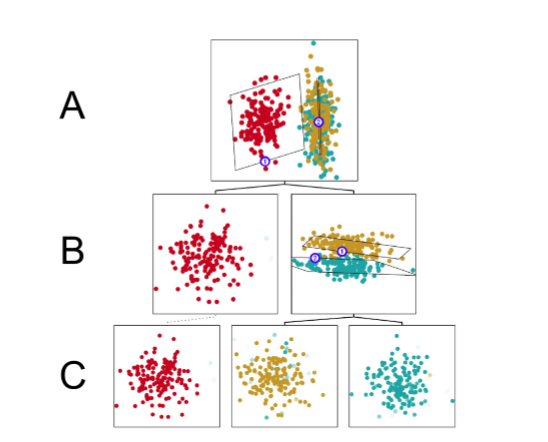
\includegraphics{figs/hierarchy_bishoptipping.png}
    \caption[Example of a hierarchical cluster structure.]{\small \textbf{Example of a hierarchical cluster structure.} \small The top-level shows the complete data-set in its latent space (A). The data is then clustered into a red and a yellow-and-blue cluster, and the latent space of each of those clusters is given (B). Doing so reveals structure within the yellow-and-blue cluster that was not visible before. This allows the cluster to be divided even further into separate yellow and blue sub-clusters (C). This figure has been copied from Bishop \& Tipping (1998) \cite{bishop1998hierarchical}.}
    \label{fig:example_hierarchy}
\end{figure}

In this case, $\mathcal{G}_i$ is the set of second-level sub-clusters $j$ that are contained within top-level cluster $i$. The complete-data log-likelihood function of this model is similar to that of a MoPPCAs model. %Note that the term $\pi_j$ is omitted. This is because the second layer of the hierarchical mixture model is initialized after the top-level MoPPCAs. Therefore, $\pi_j$ has already been estimated and so it remains constant over the whole function.

\begin{equation}\label{eq:llh_hmppca}
    \sum^n_{i=1} \sum^K_{j=1} \gamma^j_i \sum_{m=1}^{|\mathcal{G}_i|} \gamma_i^{m|j} \ln{\pi_{m|j} p(\bm{x}_i, \bm{z}_i)}%\mathcal{N}(\bm{x}_i|\bm{W}_m\bm{z} + \mu_m, \sigma^2_m\bm{I})}
\end{equation}

\section{Stan, NUTS and ADVI}\label{sec:stan}

All models described in this report have not been fitted analytically or by use of the EM algorithm as described above. Instead, all statistical models have been programmed in Stan so that they could be solved numerically. Stan is a platform for statistical modelling. An example of a PPCA model as defined in Stan is given in Appendix \ref{AP:ppca_stan}. Given a statistical model, Stan tries to find the posterior distribution of all unknown `parameters'. These parameters might be parameters in the classical sense, e.g. the mean and standard deviation of a Gaussian given the observed data. Alternatively, they might be missing variables, e.g. the latent variables explaining the observed variables. Using Stan has several advantages. It allows us to specify a model, or just its log-likelihood function, and then Stan attempts to find the optimal solution without requiring to derive the equations to find the maximum-likelihood solution to the model. This is especially useful when manipulating a statistical model, as we can adjust the model without needing to rewrite the (algorithmic) solution. Secondly, Stan makes use of samplers which not only give a point estimate for the parameter values but the entire posterior distribution of each unknown parameter. This gives us information about the uncertainty of the found solution. Stan implements two main algorithms for this. Most notably, Stan makes use of the No U-turn sampler (NUTS) (discussed in Section \ref{sec:nuts}). This is an extension of Hamiltonian Monte Carlo sampling. NUTS has the benefit over Hamiltonian Monte Carlo that it automatically determines the number of steps needed for convergence, saving computation time. The other, more recently implemented algorithm to determine the posterior of the parameters, is the automatic differentiation variational inference (ADVI) algorithm (see Section \ref{sec:advi}). This is an algorithm based upon variational inference. It selects a distribution from a variational family that is as similar as possible to the posterior. This might be less exact, but it saves a lot of computational cost without affecting the accuracy of the outcome too much. These algorithms were both utilized and compared in this project.

Stan does not stand alone, but rather, it needs to be implemented in another environment. For this project, programming was done by use of Python, in which Stan was implemented through a package called PyStan \cite{stan2018pystan}. The general workflow is as follows. Data is read in through the Python environment and a statistical model is specified in Stan. Then the model is compiled. Using the data as input, Stan is used to infer the parameters and outputs them to the Python environment. This data is then finally analyzed using Python.

\subsection{Monte Carlo sampling and NUTS}\label{sec:nuts}
Monte Carlo (\textbf{MC}) methods are a branch of sampling methods. They are forms of Markov chains, and generally entail a random trajectory through the sample space, directed by the underlying probability distribution of interest. An easy and well-known example is the Metropolis-Hastings algorithm \cite{metropolis1953equation, hastings1970monte}, where a fictive particle jumps randomly to new positions within the sample space. Based on the ratio of the probabilities of the old and new position, a new position can be accepted as a sample. If it is rejected, a jump to a new position is made. The samples drawn using this algorithm are guaranteed to converge to the underlying distribution when sampling long enough.

A drawback of this algorithm is that the number of samples necessary for convergence is sub-optimal, as the random walks through the sample space are inefficient. For this reason, other algorithms, such as Hamiltonian Monte Carlo (\textbf{HMC}), were proposed \cite{duane1987hybrid}. When using HMC, the fictive particle behaves as in a Hamiltonian dynamics simulation. A particle has a position in the sample space and a velocity. For a pre-determined number of steps of fixed step size, the particle moves in a random manner through the sample space, at the end of which the position is either accepted or rejected as a sample. This algorithm produces much more efficient random walks and is therefore less costly computationally. However, this algorithm has its own drawbacks. HMC requires manually setting a step-size parameter $\epsilon$ and a number of steps $L$. Sub-optimal values for these parameters can result in unnecessary computational cost and inaccurate results. Particularly, setting $L$ too high will result in the particle slowly returning to its original position, which requires not only unnecessary computation but also leads to slower convergence. Tuning these parameters usually requires some degree of expertise and a few tuning runs of the algorithm. Some adaptations to HMC have been proposed to automatically tune $\epsilon$ \cite{nesterov2009primal}, but not $L$.

The No-U-Turn Sampler \cite{hoffman2014no} (\textbf{NUTS}) is an extension to HMC. NUTS is most notable for its ability to determine the optimal number of steps $L$ while running. When a particle moves through the sample space to generate a sample, the number of steps needs to be high enough for a decent random walk to happen, but not too high as the fictive particle will eventually loop back and move back to its original position. The point where the fictive particle is the furthest away from its initial position is characterized by sharp turns in the path of the particle. Stopping at these `U-turns' is where the algorithm has drawn its name from. Additionally, NUTS tunes $\epsilon$ automatically whilst running the algorithm.

% To optimize the number of steps, the optimal number of necessary steps for the algorithm to run is determined while running. Each sample is initialized with the position of the previous sample and then walks a trajectory to the next sample. 
% In the optimal case, the next sample is chosen when the new sample is as far away as possible from the old sample. If the number of steps of the trajectory is set too low, the fictive particle has yet to reach this farthest point, whereas if the number of steps is too large, the particle returns in the direction of its original position, wasting both computation and decreasing the efficiency of the algorithm. 
NUTS has added a feature that checks when the sampling trajectory is at its maximum length and then uses this criterion to stop. The concrete criterion depends on the derivative of half the squared distance from the original to the new sample. If this measure is close to zero, the squared (and thus the absolute) distance between the two samples is not changing anymore and the trajectory is probably at its point of return. The series of samples is desired to be a Markov chain. One necessary property of such Markov chains is known as time-reversibility, i.e. the validity of the series of samples is not dependent on whether the samples are read from front to back or back to front. To maintain the time-reversibility of the Markov Chain, the trajectory is run both forward and backward in time. The algorithm builds a `tree' to examine the structure of the trajectory and the algorithm halts with a probability that is negatively proportional to the derivative of half the squared distance at either end of the trajectory. 
Secondly, NUTS tunes $\epsilon$ on-the-fly, based on a method named `dual averaging' \cite{nesterov2009primal}. This adaptation has been slightly improved to include more parameters. Apart from adapting $\epsilon$ while running, NUTS does a quick search for a reasonable value of $\epsilon$ to initialize the algorithm with.

 \subsection{Variational inference and ADVI}\label{sec:advi}
 Variational inference (\textbf{VI}) is a method of approximating a posterior probability distribution $p(\bm{\theta}|\bm{x})$ for the parameters $\bm{\theta}$ given data $\bm{x}$ that is difficult to determine. It works by chossing a familiy of probability distributions $q(\bm{\zeta})$ and then minimizing the dissimilarity between $P$ and $Q$. To measure this dissimilarity, the Kullback-Leibler divergence of $P$ and $Q$ ($D_{KL}(Q||P)$) is used. This is an asymmetric similarity measure defined as $D_{KL}(Q||P) = \int q(\bm{\theta}) \log{\frac{q(\bm{\theta})}{p(\bm{\theta}|\bm{x})}}$. This can be rewritten as $D_{KL}(Q||P) = \log{p(\bm{x})} - \mathcal{L}(Q)$, where $\mathcal{L}(Q) = -E_{\bm{\theta}}[\log{q(\bm{\theta})}-\log{p(\bm{\theta},\bm{x})}]$. The first term $\log{p(\bm{x})}$ is known as the evidence. The last term $\mathcal{L}(Q)$ is the evidence lower bound or \textbf{ELBO}. Its name is derived from the fact that the evidence is the sum of the ELBO and the KL divergence; since the KL divergence is non-negative, the ELBO is the lower bound for the evidence.
 Often, finding the optimal distribution $q(\bm{\zeta})$ though KL-divergence minimization is difficult or impossible. However, the evidence is a function that does not rely on $q(\bm{x})$ and is therefore kept constant as $q(\bm{x})$ is optimized. Minimizing the KL divergence is therefore equivalent to maximizing the ELBO, as is done in VI.
 
 ADVI \cite{kucukelbir2017automatic} is an algorithm that implements VI and automates the process. Traditionally, performing a VI algorithm required that the researcher had specified a VI algorithm beforehand, which included the selection of a family of variational distributions, the objective function to optimize and the computation of its gradients. This was not only an effort to the researcher, but it was also an obstacle to the automatization of the process. ADVI differs in that it transforms the given model to be suitable to a premade VI algorithm so that the aforementioned steps become obsolete.
 ADVI starts off by transforming the probability density function of the posterior. ADVI's VI algorithm assumes that all parameters live in the real space and are unconstrained, which is what is achieved by this transformation. After this transformation, ADVI's premade VI algorithm can be used for ELBO maximization.
 
 A family of variational approximations is expressed as Gaussians, either with a diagonal covariance matrix (mean field variational inference) or with a full covariance matrix (full-rank variational inference). The latter is more precise but also computationally more costly. 
The objective function to be optimized is expressed as the expectation of the distribution, which can easily be derived by sampling from the distribution and taking the empirical mean.
%  Seeing as how a variational distrbution consists out of Gaussians, computing the expectation of each distribution can be done through Monte Carlo (\textbf{MC}) integration and requires only sampling from the distribution and taking the mean of the sample.
%  Seeing as how easy it is to compute the expectation of a variational approximation, the gradient of the objective function is expressed as an expectation over $q$. This allows MC methods to easily approximate the gradient. By use of elliptical standardization, this expectation is expressed by standard Gaussians, which are easy to evaluate.
 
 The gradient of the logarithm of the joint probability distribution of the parameters and the data with respect to the parameters ($\nabla_\theta \log{q(\bm{x},\bm{\theta})}$) is computed through automatic differentiation \cite{baydin2017automatic}. Automatic differentiation is a technique to determine the gradient of a function which has been implemented in Stan (and was one of the reasons that Stan was chosen as a suitable environment for ADVI).
 Using the expectation of the gradient of the log joint probability, it is possible to obtain a noisy estimate of the gradients of the ELBO.
 The noisy gradient of the function is then used to optimize the variational distribution $q$ by stochastic gradient ascent. Finally, the ELBO has been maximized and a (local) optimum for the posterior distribution of the parameters has been found. This sequence of steps is integrated in PyStan under the name Variational Bayes (\textbf{VB}) and will be referred to under this name in this report.
 
 
 \section{Detailed description of the model}\label{sec:mode}
\subsection{The model}
Our visualization model is a hierarchical one, based on an earlier model by Bishop \& Tipping \cite{bishop1998hierarchical} (see Figure \ref{fig:example_hierarchy}). It visualizes data, and if group structures are present, it attempts to find groups within the data on the top-level, and then possibly sub-groups within the groups at the deeper levels. The model presented in this report is mainly used for visualization of data. Therefore, the model was built to find the latent space of the data on every level, so that the data could be represented in its latent dimensions. The first latent data-space, on top-level, can easily be obtained with a normal PPCA model. The result gives the projection of the data on the first two principal components. Next, a MoPPCAs model is applied to the data, which attempts to find clusters and gives their projection onto their first two principal components. From this point on, the model repeatedly applies MoPPCAs to every cluster of data for the desired number of levels. For every level, the algorithm evaluates the clusters found on the level above. First, every cluster is tested for how many sub-clusters it possibly contains. If the cluster contains two or more sub-clusters, a MoPPCAs is initialized. If the cluster contains only one sub-cluster, i.e. the cluster cannot be divided any further into sub-clusters, its branch is marked as fully analyzed. Once the MoPPCAs returns the results, we have the new latent spaces of the cluster of interest. The MoPPCAs gives us also the probabilities of all the data-points belonging to the sub-cluster $\gamma^k_i$ (see equation \ref{eq:gamma}). When all clusters have been divided into their sub-clusters, the next level is initiated, where every cluster of the last level will be attempted to split into its sub-clusters. The researcher has the possibility to select using NUTS or VB for fitting the PPCA and MoPPCAs models before initializing the model.

Note that, even though every MoPPCAs model returns the latent spaces of the found sub-clusters, the full-dimensional data is used as input to these models. The found latent data is not reused as input for later MoPPCAs models. The latent space is only used for visualization purposes (Section \ref{sec:visualization}) and for estimation of the number of sub-clusters (Section \ref{sec:n_clus}).

Clusters that are found to be fully analyzed do not undergo further evaluation on deeper levels. Instead, the latent data-set is copied over to the next level directly. When all clusters are fully analyzed or when the maximum depth of levels as specified by the researcher is reached, the model stops. A summary in pseudocode for this model is given in Algorithm \ref{alg:model}.


\begin{algorithm}[H]
 \KwData{$X$}
 \KwResult{$\bm{Z}$ and $\gamma^j_i$ for all data-points $\bm{x}_i$ and clusters $j$}
%  initialization\;
initialize $level := 0, max\_depth = 5, max\_tries = 3$\;
 Initialize top-level PPCA and plot latent projection\;
 Make every data-point part of one cluster $c$ with $\gamma^c_i=1.0$\;
 \While{$level < max\_depth$}{
 Increment $level := level + 1$\;
 \For{every cluster $c$ found in last level}{
 Find initial clustering with GMM in latent space\;
 \If{there are no sub-clusters}{
 skip to next cluster}
 \While{No MoPPCAs solution has been found}{
 Set $tries := 0$\;
 \While{$tries < max\_tries$}{
 Increment $tries := tries + 1$\;
 Initialize weighted MoPPCAs model on full-dimensional data-set with weights $\gamma^c_i$\;
 \If{MoPPCAs find model with same number of clusters as initial GMM}{
 Break loop}
 }
 \If{No MoPPCAs fit is found with same number of clusters as GMM}{
 Break loop and use MoPPCAs fit with highest number of clusters as initialization for new MoPPCAs model}
 }
 \For{every sub-cluster $sc$ found with MoPPCAs model}{
 Extract probabilties $\gamma^{sc}_i$\;
 $\gamma^{sc}_i := \gamma^{sc}_i \gamma^{c}_i$\;
 Plot found latent data-set with ink density proportional to $\gamma^{sc}_i$\;
 }
 }
 }
 \caption{Pseudocode of HmPPCAs model}
 \label{alg:model}
\end{algorithm}



\subsection{Drawing a sample}
 When NUTS is used, the user receives the samples that were generated in the process. This excludes the first warm-up samples and every other sample is thrown away as well to reduce the correlation between samples, but the other samples are returned to the user. With the settings used in this project, this left $300$ samples for the user. When VB has found its optimal posterior distribution, a sample of $1000$ points is taken from the distribution. In either case, the mean of all generated data-points is taken as the expected value of the unknown parameters. When the latent data-set or other parameters are computed, then these expected values were used.

\subsection{Initialization, priors and constraints for the MoPPCAS models}\label{sec:prios}
The MoPPCAs model was highly dependent on the initialization. This is mainly due to local optima in (soft) clustering methods. The first trials of the MoPPCAs models were performed with Stans default random initialization of parameters. This would often lead to high computation times and implausible solutions. A common result was that the algorithm would find values of $\pi_k$ that were near zero for one or more clusters. This meant that no data-points or only a few outliers were determined to be part of that cluster, which made them practically absent. Part of the reason that this happened is that a normal distribution with a very low spread can be fit to a cluster containing only one data-point with a very high likelihood. The spread of the remaining cluster(s) would be set high enough to encompass the remaining data-points. To prevent this behaviour, the initial clustering was performed by a GMM. GMMs were fitted in the latent space while varying the number of components. The optimal number of components was determined using the Bayesian information criterion (\textbf{BIC}; see Section \ref{sec:n_clus}) and was used as a reference for the MoPPCAs clusters. After the GMM clustering completed, only the most probable cluster for each data-point was noted, not the probabilities of belonging to each cluster. The values of $\mu_k$ and $\sigma_k$ were inspired by the values of the centers and the spread of the clusters as found by the GMM. Because the GMM clustering was performed in the latent space, the labeling of the data-points to their clusters had to be applied to the same data-points in the full-dimensional space first. This way, the center and covariance matrix of each cluster could be estimated in the full-dimensional space. Basing $\sigma^2$ on the covariance matrix of the clusters is not entirely correct, because the covariance matrix of the PPCA model is $\bm{W}\bm{W}^T + \sigma^2 \bm{I}$. Directing the value of $\sigma^2$ to values based on the found covariance matrix would actually overestimate $\sigma^2$, which in turn would lead to underestimation of $\bm{W}$. However, the resulting inference of the model would be off without doing so. Therefore, after trying various alternatives, the following three steps were taken to direct $\sigma^2$ to the spread of the clusters as found by the GMM.

First of all, the centers and the spread of the clusters that were found by the GMM were used to initialize parameters $\mu_k$ and $\sigma_k$ in the MoPPCAs model. Values for $\pi_k$ were computed from the GMM solution and used as initial values for $\pi_k$ similarly. The solution of the GMM was also used to initialize $\gamma^k_i$ for all values as  $1$ (when $i$ belonged to $k$ according to the GMM) or $0$ (otherwise). It was then evaluated whether the problem where few to no data-points were assigned to a cluster was avoided. The problem was solved for low-dimensional data-sets, but the problem persisted when more complex data-sets were analyzed. Another reason for this initialization was that a random initialization would lead to random labeling of clusters. This would lead to inconsistencies in cluster labels between samples and affect the outcome negatively. A consistent initialization meant also that the label-swapping problem during clustering was solved.

Secondly, a prior was set over $\mu_k$ and $\sigma_k$, to direct the parameters towards the correct solution. For $\mu_k$, a prior was specified in the form of a normal distribution that was fit to the points that the GMM had labeled to cluster $k$ in the full-dimensional space. As a prior for the standard deviation of the clusters, an inverse gamma distribution, fit with help of the GMM solution, was specified at first, but this seemed to worsen the results. A normal distribution was then specified as a prior as this yielded better results. Since $\sigma_k$ is a single value related to the spread in all dimensions within that cluster, the mean of the diagonal of the covariance matrix of a cluster was used as the expectation of $\sigma_k$, thus $E[\sigma_k] = \frac{1}{d}Tr(\Sigma^{GMM}_k)$ with $\Sigma^{GMM}_k$ being the covariance matrix of GMM cluster $k$.
% The standard deviation of the prior distribution was set to be the standard deviation of all diagonal entries in $\Sigma^{GMM}_k$.
This approach saved computational cost, but it did not necessarily prevent the problem discussed above.

Since the problem of empty clusters resulted in clusters with a minimal or large spread, constraints were set on the standard deviations of the MoPPCAs clusters in the data space. Therefore, a lower bound on $\sigma_k$ was set of $0.75$ times the standard deviation of the GMM cluster in the dimension with the lowest spread. This did not prevent the problem, as there could still be clusters with near-zero $\pi_k$, while other clusters took over their data-points by increasing their $\sigma_k$. Therefore, an upper bound was also set on the value of $\sigma_k$. This upper bound was set to be $1.25$ times the standard deviation of the GMM cluster in the dimension with the largest spread. Stan does not accept different constraints on the entries of one vector and our lower and upper bounds were different for every cluster. As a solution, \textit{raw} vectors of $\bm{\mu}_k$ and $\sigma_k$ were evaluated as normalized vectors with entries between $0$ and $1$. Now, they all had the same upper and lower bounds ($1$ and $0$). These normalized values were then later in the model transformed to their real values by multiplying them with the difference between the upper and lower bound values and adding the lower bound values to them.

Using all these constraints put the initial GMM solution largely in charge of the clustering part of the MoPPCAs solution, leaving the MoPPCAs model to make only minor adjustments to the clustering of the full-dimensional space. Despite this, it still happened occasionally that `empty' clusters were found and that the MoPPCAs model found a different optimal clustering with fewer clusters. This was not necessarily a problem on the side of the MoPPCAs model, because overestimation of the number of clusters also happened from time to time (see Section \ref{sec:n_clus}). If this happened three times in a row, the MoPPCAs solution with the highest found number of clusters was accepted. However, because this model was initialized with a prior directed at a different solution, a second MoPPCAs model was initialized with the newly found number of clusters. All initial values were copied from the first MoPPCAs model, and priors and constraints on the model were taken from the first MoPPCAs solution in the same way that they were taken from the initial GMM for the first MoPPCAs model.

\subsection{Dealing with responsibility terms on the deeper levels}
When analyzing a cluster, every data-point $i$ has a responsibility term $\gamma^k_i$, describing the probability of belonging to cluster $k$. Therefore, all data-points are input to the MoPPCAs, even the ones that probably don't belong in this cluster, albeit with a very low weight. These numbers are passed into the MoPPCAs to be used in the expected complete-data log-likelihood of equation \ref{eq:llh_hmppca}. For the first level, $\gamma^k_i = 1$ for all data-points, meaning that every data-point starts as being part of the same cluster with complete certainty. When we move to deeper levels, the likelihood equation changes from \ref{eq:llh_hmppca} to \ref{eq:llh_hmppca2}, where $l$ sums over the sub-clusters at the next level.

\begin{equation}\label{eq:llh_hmppca2}
    \sum^n_{i=1} \sum^{K_1}_{j=1} \gamma^j_i \sum^{|\mathcal{G}_j|}_{l=1} \gamma^{l|j}_i \sum_{m=1}^{|\mathcal{G}_l|} \gamma^{m|j,l}_i \ln{\pi_{m|j,l} p(\bm{x}_i,\bm{z}_i)}
\end{equation}

Noting that $\gamma^j_i \gamma^{l|j}_i = \gamma^{j,l}_i$ we can rewrite \ref{eq:llh_hmppca2} back to \ref{eq:llh_hmppca}, where now $j$ denotes the sub-clusters on the next level. We can, therefore, reuse the same MoPPCAs model, but this time inputting the probabilities of belonging to the new sub-clusters as $\gamma^j_i$. Every MoPPCAs returns $\gamma^{l|j}_i$. Seeing as how $\gamma^j_i \gamma^{l|j}_i = \gamma^{j,l}_i$, we just have to multiply this number with the probability of belonging to the cluster on the level above to obtain the probability of belonging to the new sub-cluster, which will be the input responsibility term for the next level. Therefore, the model initializes a vector of ones of length $n$ as the responsibility terms, inputs it to the MoPPCAs model and then multiplies it element-wisely with the output responsibility terms to obtain the new responsibility terms used for the MoPPCAs for the new sub-clusters on the next level.


\subsection{BIC score to assess the number of clusters}\label{sec:n_clus}
The number of clusters to be found was estimated using the Bayesian information criterion (\textbf{BIC}). The data was clustered by a GMM with various values for the number of clusters. For the GMM models, a ready-to-use GMM package 'GaussianMixture' from the `Sklearn' package was used, as it worked faster than Stan and we needed only a simple estimate for initialization, not the whole posterior of all parameters. Data-points were assigned to the plot with their highest responsibility term and only the points assigned to a plot were included in the GMM. These GMMs were estimated on the latent data. Although the full-dimensional data may contain more information, it also contains more noise and we found that better estimates were therefore obtained from using the latent data. The maximum number of clusters to be found, $K_{max}$, was set relatively low to $K_{max} = 3$. This lead to the need for multiple levels in our models, to get a better grasp of the hierarchical working of the model. The minimum number of clusters to be found $K_{min}$ was always set to $1$, except for the top-level, where it was set to $2$ to stimulate the model to make at least one division in the data-set. For each value of $K$, three GMM models were fit to the data, although users can choose to fit as many GMM models as they like. Pseudocode for this process is given in algorithm \ref{alg:n_clus}. Note that $Z$ in this algorithm contains not all data-points in the latent space, but only the ones that were assigned to the plot which is analysed. 

The BIC of a model fit is defined as $BIC = k \ln{n} - 2 \ln{\mathcal{L}}$, where $n$ is the number of data-points, $k$ the number of clusters and $\mathcal{L}$ the likelihood. The likelihood of a GMM model is defined in Appendix \ref{app:gmm_em}. For each model, the BIC was computed, and the model with the lowest BIC was chosen as the best suitable model for the data.
% Not only was the number of optimal sub-clusters directed to the following MoPPCAs model, the model was also initialized with all data-points labeled accordingly to the best found GMM model. The mean and standard deviations of all clusters were also given to the model, after being recomputed in the original, full space. 

Even though the BIC score usually gave a very good estimate for the number of sub-clusters, it happened from time to time that the MoPPCAs found fewer clusters. In these cases, the responsibilities were all approaching $0$ for every data-point for that cluster. If a sub-cluster $j$ was not assigned any data-point $i$ (i.e. $\text{argmin}_k \gamma^k_i) \neq j~\forall i$), the MoPPCAs was retried for up to three times. If the suggested number of sub-clusters was still not found by the third time, a new MoPPCAs model was initialized that looked for fewer sub-clusters. After all, it is possible for the GMM to over-estimate the number of sub-clusters. Under-estimation of the number of sub-clusters is not a problem since the found sub-clusters will be analyzed further at deeper levels.

\begin{algorithm}[H]
 \KwData{$Z$, $K\_min$, $K\_max$, $n\_ref$}
 \KwResult{GMM fit on $Z$ with optimal number of clusters}
Initialize $k = K\_min$\;
 \While{$k \leq K\_max$}{
 set $ref := 0$\;
 \While{$ref < n\_ref$}{
 increment $ref := ref + 1$\;
 Cluster $Z$ into $k$ clusters using GMM\;
 Compute likelihood $L$ of the resulting GMM fit\;
 Compute the BIC as $BIC := k \ln{n} - 2 \ln{L}$\;
 }
 }
 Return GMM fit with lowest BIC\;
 \caption{Determining the number of clusters}
 \label{alg:n_clus}
\end{algorithm}

\chapter{Methods}\label{sec:methods}
\lhead{\emph{Methods}}

\section{Data description}\label{sec:data}
Two types of data-sets were used. The first type consisted of simulated data-sets generated using Splatter \cite{zappia2017splatter}. This is an R-package that allows the user to generate customized scRNA-seq data-sets. Since Splatter data-sets are easily obtainable and customizable, two different types of data-sets were generated: one simple type which contained five groups of cells that were easy to differentiate from each other and one complex type containing six groups of cells which showed more overlap in their patterns. The difference in complexity of these data-sets was regulated by use of the `de.facLoc', `de.facScale' and the `de.prob' parameters. These parameters describe how easily diffent groups can be separated. The last parameter `de.prob', the probability with which genes in a group were differentially expressed, was set higher for the complex data-sets than for the simple data-sets, as the different groups of cell-types were not distinguishable without doing so. For the simple Splatter data-sets, de.prob was set higher for the data-sets containing fewer genes, to make sure that each data-set contained enough differentially expressed genes. For the complex Splatter data-sets, this was not necessary, as de.prob was high enough already for even the data-set containing 5 genes. For both the simple and the complex types of data-sets, data-sets of 5, 25, 50, 150 and 250 genes were created.

The other type of data-sets, were the scRNA-seq data-sets published by Darmanis \textit{et al.} (2015)\footnote{retrieved from \url{https://hemberg-lab.github.io/scRNA.seq.datasets/human/brain/}} \cite{darmanis2015survey} and Nestorowa \textit{et al.} (2016)\footnote{retrieved from \url{http://blood.stemcells.cam.ac.uk/single_cell_atlas.html}} \cite{nestorowa2016single}. They have respectively measured the expression of 22088 and 4774 genes across 466 and 1656 cells. The Darmanis samples were retrieved from adult and fetal human brain tissue and the samples from the Nestorowa data-set were obtained from mouse hematopoietic stem and progenitor cells. The Darmanis data-set was labeled by ten different cell types: groups of oligodendrocyte precursor cells, oligodendrocytes, astrocytes, microglia, neurons, endothelial cells, fetal replicating cells, fetal quiescent cells, a hybrid group of cells and unannotated cells. The Nestorowa data-set was labeled with three different cell types: progenitor cells, hematopoietic stem and progenitor cells (\textbf{HSPC}) and long-term hematopoietic stem cells (\textbf{LT\_SHC}). The Darmanis data-set was transformed by taking $\log{(\bm{X}}+1)$. The Nestorowa data-set was used as is as the authors had normalised the gene counts themselves according to the method described by Lun \textit{et al.} (2016) \cite{lun2016pooling}. To save computational cost, these data-sets were filtered to include only the 500 genes that showed the largest variance.
All data-sets are described in Table \ref{tab:datasets}.

\small

\begin{table}
\caption[Properties of the gene expression data-sets.]{\textbf{Properties of the gene expression data-sets.}}
    \centering
    \small
    \begin{tabular}{l|r|r|r|r|r|r}
     & Genes & Cells & cell types & de.prob & de.facLoc & de.facScale\\
    \hline
    \multirow{5}{*}{\makecell{Simple\\Splatter}} & 5 & 500 & 5 & 0.5 & 3 & 0 \\
      & 25 & 500 & 5 & 0.1 & 3 & 0 \\
       & 50 & 500 & 5 & 0.05 & 3 & 0 \\
       & 150 & 500 & 5 & 0.017 & 3 & 0 \\
        & 250 & 500 & 5 & 0.01 & 3 & 0 \\
    \multirow{5}{*}{\makecell{Complex\\Splatter}} & 5 & 750 & 6 & 0.5 & 0.1 & 0.4 \\
      & 25 & 750 & 6 & 0.5 & 0.1 & 0.4 \\
       & 50 & 750 & 6 & 0.5 & 0.1 & 0.4 \\
       & 150 & 750 & 6 & 0.5 & 0.1 & 0.4 \\
        & 250 & 750 & 6 & 0.5 & 0.1 & 0.4 \\
    Darmanis & \makecell{500 (out\\of 22088)}& 466 & 9 & - & - & - \\
    Nestorowa & \makecell{500 (out\\of 4774)}& 1656 & 3 & - & - & - \\
    \end{tabular}
    \label{tab:datasets}
\end{table}

\normalsize

\section{Programming environment}
For this project, programming was done by use of Python (Python 3.8.2-1), with the statistical models specified in Stan using the PyStan package (Pystan 2.19.1.1) \cite{stan2018pystan} on a machine running Arch Linux 5.5.13. Stan models were compiled using the GCC compiler (GCC 9.3.0-1).


\section{Experiment set-up}
All data-sets were evaluated using the HmPPCAs model, using both NUTS and VB. The parameter settings were kept constant for all data-sets. These parameter settings are given in Table \ref{tab:params}.

\begin{table}
\caption[Parameter settings of the HmPPCAs model.]{\textbf{Parameter settings of the HmPPCAs model.}}
    \centering
    \begin{tabular}{l|l|c}
        Parameter & Comments & value \\
        \hline
        \textbf{General} & & \\
        M & Number of latent dimensions & 2 \\
        max\_depth & Maximum number of levels before termination & 5\\
        min\_clus\_size & \makecell[l]{If a cluster contains less than this number\\of data-points, it is not divided\\into further sub-clusters anymore} & 10 \\
        n\_try & \makecell[l]{Number of trials to find a MoPPCAs fit\\with the adequate number of clusters} & 3\\
        k\_max & Maximum number of sub-clusters per cluster & 3\\
         & & \\
        \textbf{NUTS} & & \\
        iterations & Number of iterations & 300\\
        chains & Number of Markov chains running simultaneously & 1\\
        warmup & \makecell[l]{Number of steps used for step-size\\adaptation but not for inference} & 150\\
        thin & \makecell[l]{Number of samples skipped between saved samples,\\to reduce the correlation between successive samples} & 1\\
        & & \\
        \textbf{ADVI} & & \\
        iterations & Number of iterations & 10000\\
        algorithm & Mean field or Full-rank & Mean field\\
        & & \\
        \textbf{Visualization} & & \\
        vis\_theshold & \makecell[l]{Points that are part of a cluster with a\\probability lower than this are not plotted} & 0.05\\
    \end{tabular}
    % \medskip
    \small
    These settings were maintained for all data-sets.
    \label{tab:params}
\end{table}

The performance of the model was evaluated on all data-sets described in section \ref{sec:data}. Performance, as well as the computation time, was measured both when using NUTS and VB (section \ref{sec:performance_measures}). Performance was also measured when using UMAP \cite{mcinnes2018umap} and t-SNE \cite{maaten2008visualizing} as a baseline. For this, the UMAP package (UMAP 0.4) \cite{mcinnes2018umap} and the `sklearn' package `TSNE' were used. All parameters were left at their defaults, except for the perplexity parameter for t-SNE. Multiple values for the perplexity were tried, a value of $30.0$ was found to yield the best results for the Splatter data-sets, a perplexity value of $50.0$ was used when analyzing the Darmanis and Nestorowa data-sets. The performance at the top-level was also recorded to represent a standard PPCA method.

\subsection{Visualization}\label{sec:visualization}
After every level, including the top-level which initializes a PPCA on the complete data-set, the latent data is gathered for every group. For every level, the latent data can then be plotted for every cluster. All data-points are plotted in every plot, but the responsibility terms determine the density of the ink with which the points are plotted. This has the effect that most data-points are plotted only in the plot that portrays the latent space of the cluster they belong to, with the occasional data-point being vaguely represented in multiple plots that the data-point might belong to with lesser certainty.

\subsection{Performance measures}\label{sec:performance_measures}
Because the main purpose of the model was to help with visualization, the plots are being evaluated in terms of how well cell types could be separated. In the optimal case, the model produces plots in which the different cell-types are clearly separated from each other into individual clusters, possibly creating even better plots on deeper levels. To evaluate the visual separability of the cell-types, a multinomial logistic regression model was used. The logistic regression from the `sklearn' package `LogisticRegression' was used for this and `lbfgs' was used as its optimization algorithm. For every plot on every level, a logistic regression was performed within a $5$-fold cross-validation scheme. Technically, all points appear in every plot with a non-zero probability, but the points were only used for the logistic regression in the plot that they appeared in with the highest probability. In practice, most points appear with a probability of almost $1$ in one plot and with a probability close to $0$ in the other plots, so the effect of this categorization of data-points into plots is minimal. The data-points were always divided into five folds of approximately equal summed responsibility terms. The accuracy was then measured from these results. The final accuracy taken as evaluation for the individual plot was the average of the accuracies of the five test-sets. The accuracy for the whole level was given by the weighted accuracy of all the plots within that level, where the ratio of data-points in a plot was used as its weight.
When reporting the accuracy of the model on an entire data-set, the level with the highest accuracy was used as a reference. This was usually the deepest level.

Apart from the visualization evaluation, the time it took to perform each analysis was also recorded. Whenever a model in Stan would be initialized or finished, the time was noted, so that the difference between the finishing time and start time could be reported as the computational time of a model. This included the individual times of the top-level PPCA. UMAP and t-SNE were left out of this comparison, as these techniques were used to create a single visualization result, so this would be an unfair comparison with inference techniques that produced the entire posterior distribution of all parameters. Because the computation time to fit a complete HmPPCAs model is highly dependent on the number of levels of the model and the number of mixture components that the data-set consists of, the computation time of the individual MoPPCAs models within the HmPPCAs was measured rather than the time it took to solve the whole HmPPCAs model. The number of mixture components that a MoPPCAs model was trying to find was noted to see if it had an effect on the computation time. Sometimes the number of mixture components that a MoPPCAs model had found was lower than the number of mixture components that it was trying to find. For these cases, both the number of mixture components the model was looking for as suggested by the initial GMM (Section \ref{sec:n_clus}) and the number of mixture components as found by the MoPPCAs were noted.

\chapter{Results}\label{sec:results}
\lhead{\emph{Results}}

In this section, we will discuss the results found during the experiments. As mentioned in Section \ref{sec:performance_measures}, two performance measures were taken into account. First, we will report the accuracy scores as found by the visualization assay. This will be a measure of how good a dimensionality reduction technique was at portraying the data in two dimensions while preserving most information. Secondly, the time it took to perform these analyses are reported. Here we will evaluate the time-wise computational cost and scalability of NUTS and VB and compare them with each other.

\section{Visualization performance}
We start with the results of the visualization assay. A logistic regression was performed on each latent data-set plot to predict cell-types in the plots, where the accuracy of this result was noted. This was done using a $5$-fold cross-validation scheme. The average accuracy of the five folds was taken as the accuracy of a plot. In the case of the HmPPCAs models, the accuracy was computed for each level. Since the levels contained multiple plots, the accuracy of one level was computed as the weighted average of each plot within that level, where the weights were determined by the number of data-points that were contained within each plot. When the overall accuracies of HmPPCAs models are reported, the accuracy of the best performing level is given.

% \begin{wrapfigure}{l}{0.35\textwidth}
%   \begin{center}
%     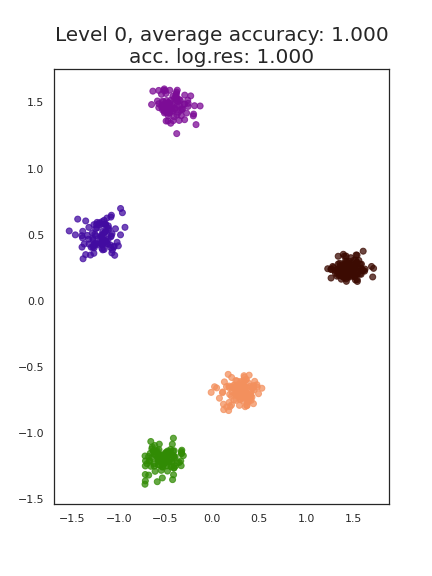
\includegraphics[width=0.35\textwidth]{figs/simple_5_nuts.png}
%   \end{center}
%   \caption{Birds}
% \end{wrapfigure}

% \begin{wrapfigure}{r}{0.35\textwidth}
%   \begin{center}
%     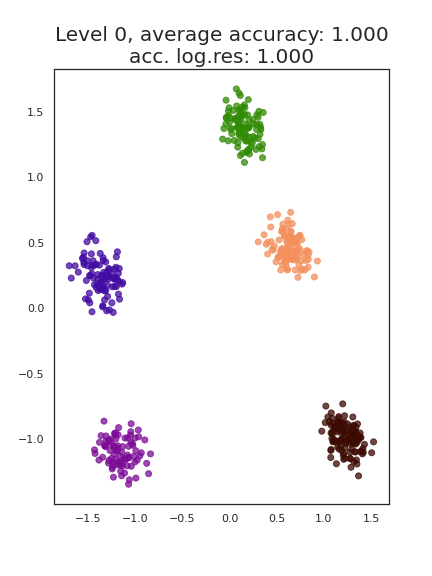
\includegraphics[width=0.35\textwidth]{figs/simple_5_vb.png}
%   \end{center}
%   \caption{Birds}
% \end{wrapfigure}

\begin{table}
\setlength{\tabcolsep}{3pt}
\caption[Accuracy of multinomial logistic regressions on the latent data-sets found by each model in a $5$-fold cross-validation scheme.]{\textbf{Accuracy of multinomial logistic regressions on the latent data-sets found by each model in a $5$-fold cross-validation scheme. The highest accuracy for a particular data-set is indicated in bold.}}
    \label{tab:results}
    \centering
    \small
    \begin{tabular}{l|rrrrr|rrrrr|r|r}
          & \multicolumn{5}{r}{Splatter simple} & \multicolumn{5}{r}{Splatter complex} & Darmanis & Nestorowa \\
          genes & 5 & 25 & 50 & 150 & 250 & 5 & 25 & 50 & 150 & 250 & 500 & 500 \\
          \hline
        
        \makecell{PPCA\\(NUTS)} & \textbf{1.00} & 0.88 & 0.99 & 0.97 & 0.94 &
        0.80 & 0.68 & 0.82 & 0.81 & 0.77 & 0.60 & 0.73\\
        
        \makecell{HmPPCAs\\(NUTS)} & \textbf{1.00} & \textbf{1.00} & \textbf{1.00} & 0.97 & \textbf{1.00} &
        0.90 & 0.82 & 0.89 & 0.82 & 0.77 & 0.70 & 0.79\\
        
        \makecell{PPCA\\(VB)} & \textbf{1.00} & 0.88 & 0.99 & 0.96 & 0.94 &
        0.80 & 0.69 & 0.81 & 0.82 & 0.76 & 0.73 & 0.73\\
        
        \makecell{HmPPCAs\\(VB)} & \textbf{1.00} & \textbf{1.00} & \textbf{1.00} & 0.98 & \textbf{1.00} &
        0.90 & 0.91 & 0.90 & 0.94 & 0.79 & 0.73 & 0.79\\
        
        UMAP & \textbf{1.00} & \textbf{1.00} & \textbf{1.00} & \textbf{1.00} & \textbf{1.00} &
        0.95 & \textbf{0.98} & 0.98 & \textbf{1.00} & \textbf{1.00} & \textbf{0.82} & \textbf{0.82}\\
        
        t-SNE & \textbf{1.00} & \textbf{1.00} & \textbf{1.00} & \textbf{1.00} & \textbf{1.00} & 
        \textbf{0.95} & 0.94 & \textbf{1.00} & \textbf{1.00} & \textbf{1.00} & 0.76 & 0.80\\
    \end{tabular}
    % \medskip
    % \small
    % The table shows the accuracy of a 5-fold cross validation scheme when performing a logistic regression on the latent data. In case of the hmPPCAs models, the weighted average accuracy of all plots on a level was taken and the accuracy on the level with the highest accuracy is shown. For PPCA, PPCA on the top-level of hmPPCAs was used.
\end{table}




\begin{figure}
    \centering
    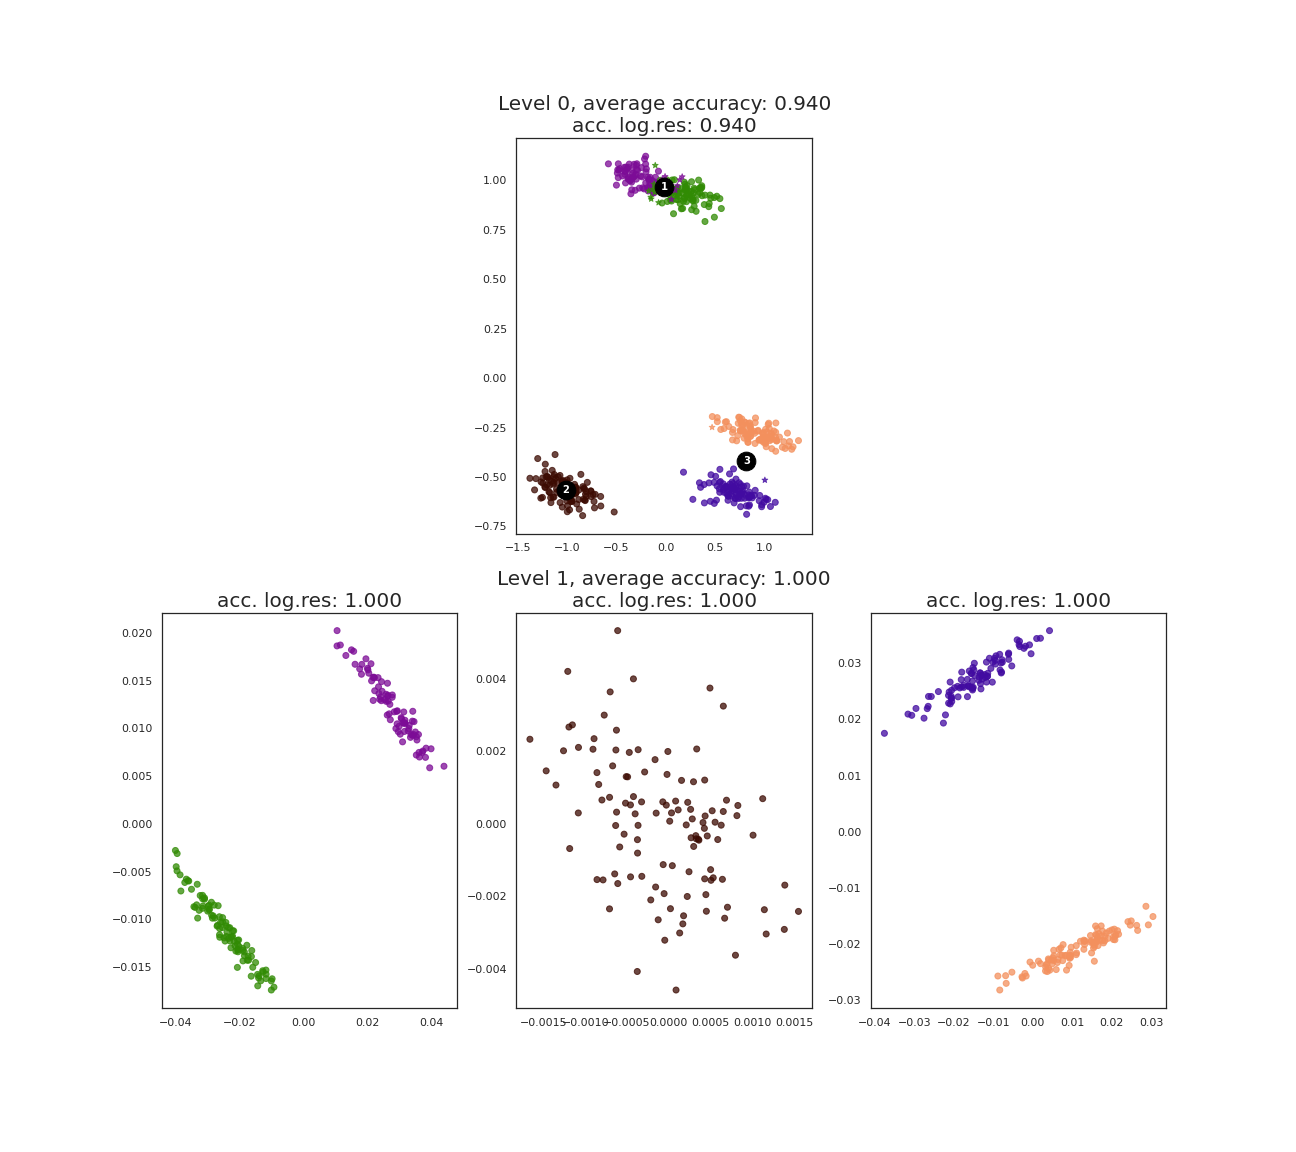
\includegraphics[width=\linewidth]{figs/simple_250_nuts.png}
    \caption[HmPPPCAs model performed on the simple Splatter data-set with 250 genes using NUTS]{\small \textbf{HmPPPCAs model performed on the simple Splatter data-set with 250 genes using NUTS.} \small The maximum accuracy of $1.0$ was found at level $1$. The top-level PPCA achieved an accuracy of $0.940$. The clusters found within the top-level PPCA have been numbered. The colours indicate different cell types. Data-points that were predicted correctly by the logistic regression are plotted with dots, incorrect predictions are plotted with stars.}
    \label{fig:simple_250_nuts}
\end{figure}



\begin{figure}
    \centering
    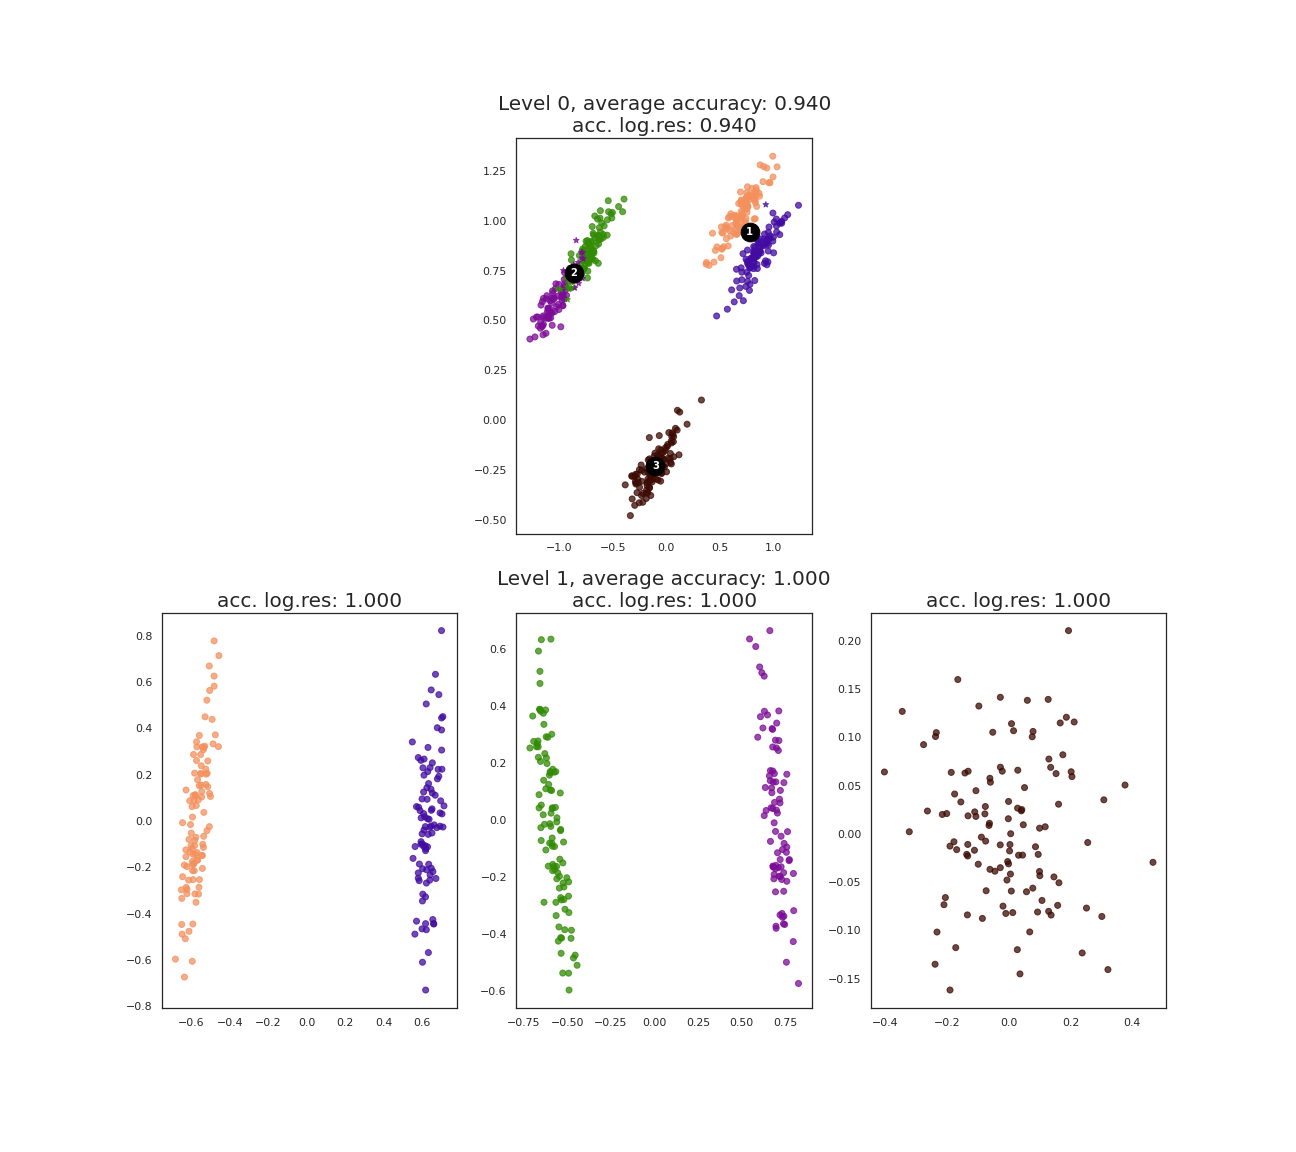
\includegraphics[width=\linewidth]{figs/simple_250_vb.png}
    \caption[HmPPPCAs model performed on the simple Splatter data-set with 250 genes using VB]{\small \textbf{HmPPPCAs model performed on the simple Splatter data-set with 250 genes using VB.} \small The maximum accuracy of $1.0$ was found at level $1$. The top-level PPCA achieved an accuracy of $0.940$. The clusters found within the top-level PPCA have been numbered. The colours indicate different cell types. Data-points that were predicted correctly by the logistic regression are plotted with dots, incorrect predictions are plotted with stars.}
    \label{fig:simple_250_vb}
\end{figure}

All results found are given in Table \ref{tab:results}. The simple Splatter data-sets were converted to their top-level latent spaces first by PPCA. Figure \ref{fig:simple_250_nuts} shows the results on the simple Splatter 250 genes data-set when using NUTS and Figure \ref{fig:simple_250_vb} shows the results when using VB. The figures for the data-sets containing fewer genes are given in Appendix \ref{sec:simple}. We see that reasonable accuracy scores ($>0.88$) were achieved on the visualization assay on the top-level latent data. When more levels of depth were added by use of the HmPPCAs, these accuracy scores almost always rose to $1.0$.

When evaluating the complex Splatter data-sets, lower and more varying accuracies were observed. The results when analysing the 250 genes complex data-set are shown in Figure \ref{fig:complex_250_nuts} (NUTS) and Figure  \ref{fig:complex_250_vb} (VB). The results of the lower dimensional data-sets are given in Appendix \ref{sec:complex}. When comparing PPCA and HmPPCAs, we see that the addition of more levels increased the accuracy in almost every case, although neither was able to achieve perfect accuracy scores on the complex data-sets. When we compare NUTS and VB, we see that their results are very similar when performing the PPCA. Occasionally, the scores of NUTS and VB differed, but the difference was always negligible. In the case of the HmPPCAs, however, larger differences between NUTS and VB were observed. VB performed better than or at least as good as NUTS in all cases when comparing the HmPPCAs results.

Both methods achieved lower scores on the Darmanis and Nestorowa data-sets than on the Splatter data-sets. Figures \ref{fig:damanis_nuts} and \ref{fig:darmanis_vb} show the result of the HmPPCAs on the Darmanis data-set when using NUTS and VB, respectively. Figures \ref{fig:nestorowa_nuts} and \ref{fig:nestorowa_vb} are the NUTS and VB HmPPCAs results when analyzing the Nestorowa data-set. The HSPC cell types in this data-set showed multiple clusters. When using NUTS, the HmPPCAs separated each of those clusters. The progenitor and LT.HSC cells were difficult to distinguish from each other. When using VB, fewer levels were initialized and therefore the data was separated less. Since a higher accuracy was achieved using NUTS on level $2$, it might have been the case that NUTS was able to obtain a slightly better visualization which led to further clustering. Again, HmPPCAs scored higher than PPCA on the Nestorowa data-sets with both NUTS and VB and on the Darmanis data-set when using NUTS. The addition of more levels did not improve the accuracy on the Darmanis data-set when using VB. VB yielded better results than NUTS on the Darmanis data-set, but both methods performed exactly equally on the Nestorowa data-set.



\begin{figure}
    \centering
    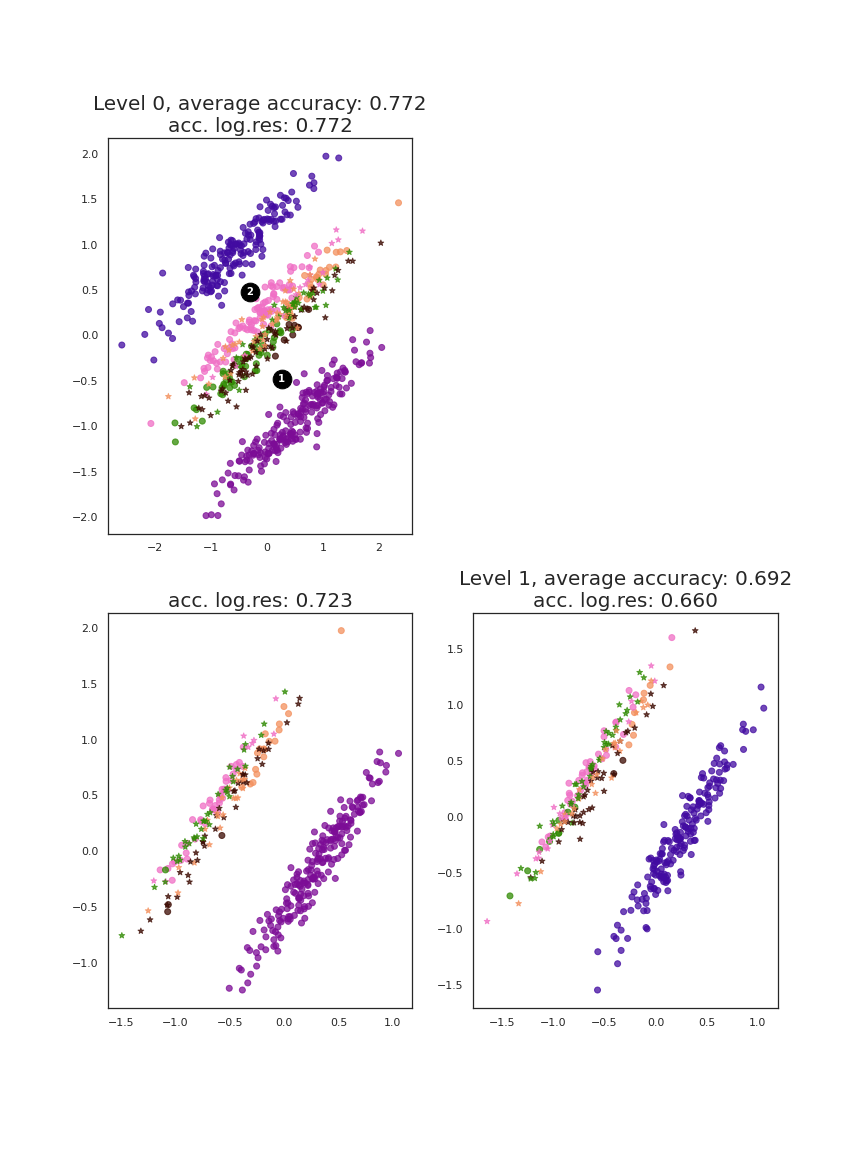
\includegraphics[width=.6\linewidth]{figs/complex_250_nuts.png}
    \caption[HmPPPCAs model performed on the complex Splatter data-set with 250 genes using NUTS]{\small \textbf{HmPPPCAs model performed on the complex Splatter data-set with 250 genes using NUTS.} \small A maximum accuracy of $0.772$ was found at level $0$. Performance did not improve after the top-level PPCA. The clusters found within the top-level PPCA have been numbered. The colours indicate different cell types. Data-points that were predicted correctly by the logistic regression are plotted with dots, incorrect predictions are plotted with stars.}
    \label{fig:complex_250_nuts}
\end{figure}


\begin{figure}
    \centering
    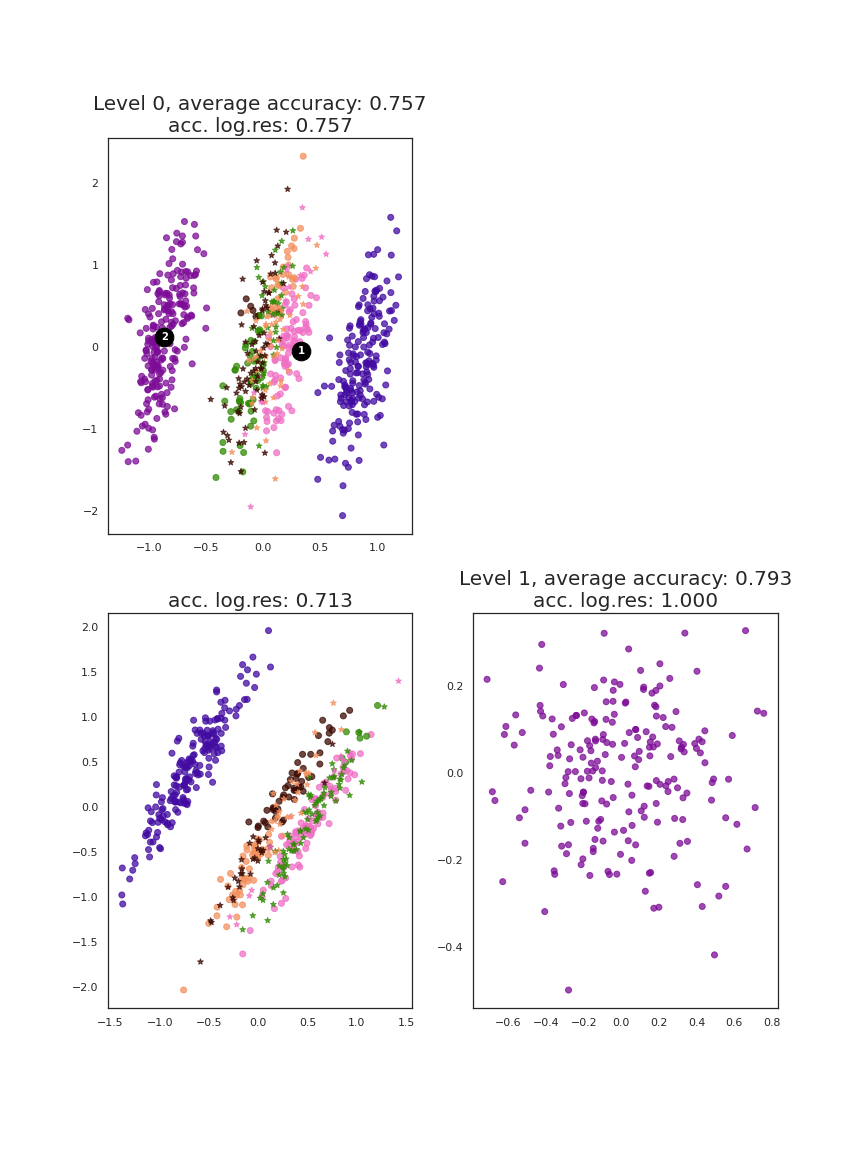
\includegraphics[width=.6\linewidth]{figs/complex_250_vb.png}
    \caption[HmPPPCAs model performed on the complex Splatter data-set with 250 genes using VB]{\small \textbf{HmPPPCAs model performed on the complex Splatter data-set with 250 genes using VB.} A maximum accuracy of $0.793$ was found after one level. The top-level PPCA achieved an accuracy of $0.757$. The clusters found within the top-level PPCA have been numbered. The colours indicate different cell types. Data-points that were predicted correctly by the logistic regression are plotted with dots, incorrect predictions are plotted with stars.}
    \label{fig:complex_250_vb}
\end{figure}


The UMAP and t-SNE baselines also achieved perfect accuracies of $1.0$ on the simple splatter data-sets. Slightly lower accuracies were achieved on the complex Splatter data-sets of low dimensionality, but this accuracy rose back to $1.0$ for the complex Splatter data-sets that contained at least $150$ genes. UMAP and t-SNE performed almost exactly equally good on the 5 genes complex data-sets, with t-SNE outperforming UMAP barely by a negligible difference. UMAP scores slightly higher on the 25 genes complex data-set and t-SNE on the 50 genes complex data-set. Together UMAP and t-SNE achieved the highest accuracy scores on the Splatter data-sets. The resulting visualizations of UMAP and t-SNE are given in Appendix \ref{sec:baselineresults}.

The result when using UMAP on the Darmanis data-set is given in Figure \ref{fig:darmanis_umap}, and the t-SNE result is given in Figure \ref{fig:darmanis_tsne}. Both of these methods outperformed the HmPPCAs. UMAP achieved the highest accuracy for the Nestorowa data-set, of which the results are visualized in Figure \ref{fig:nestorowa_nuts} (NUTS) and Figure \ref{fig:nestorowa_vb} (VB). In this case, however, t-SNE performed only slightly better than the two HmPPCAs models, and the UMAP accuracy was not much higher than the others.


% \textbf{Splatter data-sets}\\
% Figure \ref{fig:res_splatter} depicts the accuracies achieved on all splatter data-sets by the hmPPCA and the UMAP baseline. \todo{write more}

% \begin{figure}
%     \centering
%     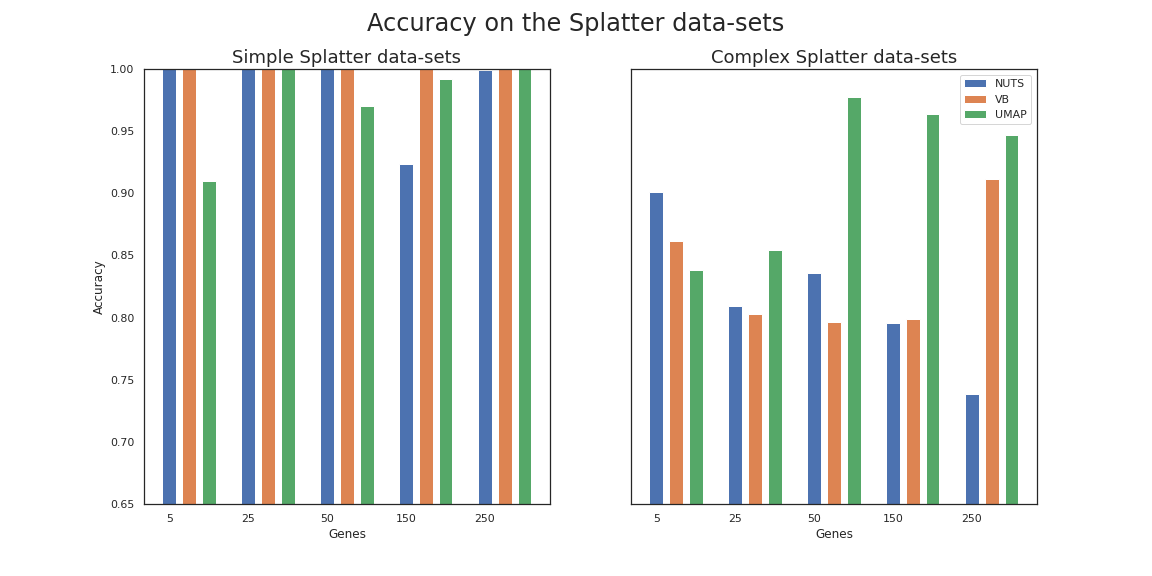
\includegraphics[width=\linewidth]{figs/Splatter_Accuracy_all.png}
%     \caption{\textbf{Accuracy on the simple (left) and complex (right) Splatter data-sets for all methods.} Accuracy is given on the y-axis and the number of genes in the data-set on the x-axis. Accuracy was measured after performing a logistic regression with a 5-fold cross validation. The results obtained through the hmPPCA are given in blue (when using NUTS) and orange (when using VB), the results of UMAP are plotted in green.}
%     \label{fig:res_splatter}
% \end{figure}
% \todo{needs to be updated, complex250 set is incorrect}

% \textbf{Damanis data-set}\\

\begin{figure}
    \centering
    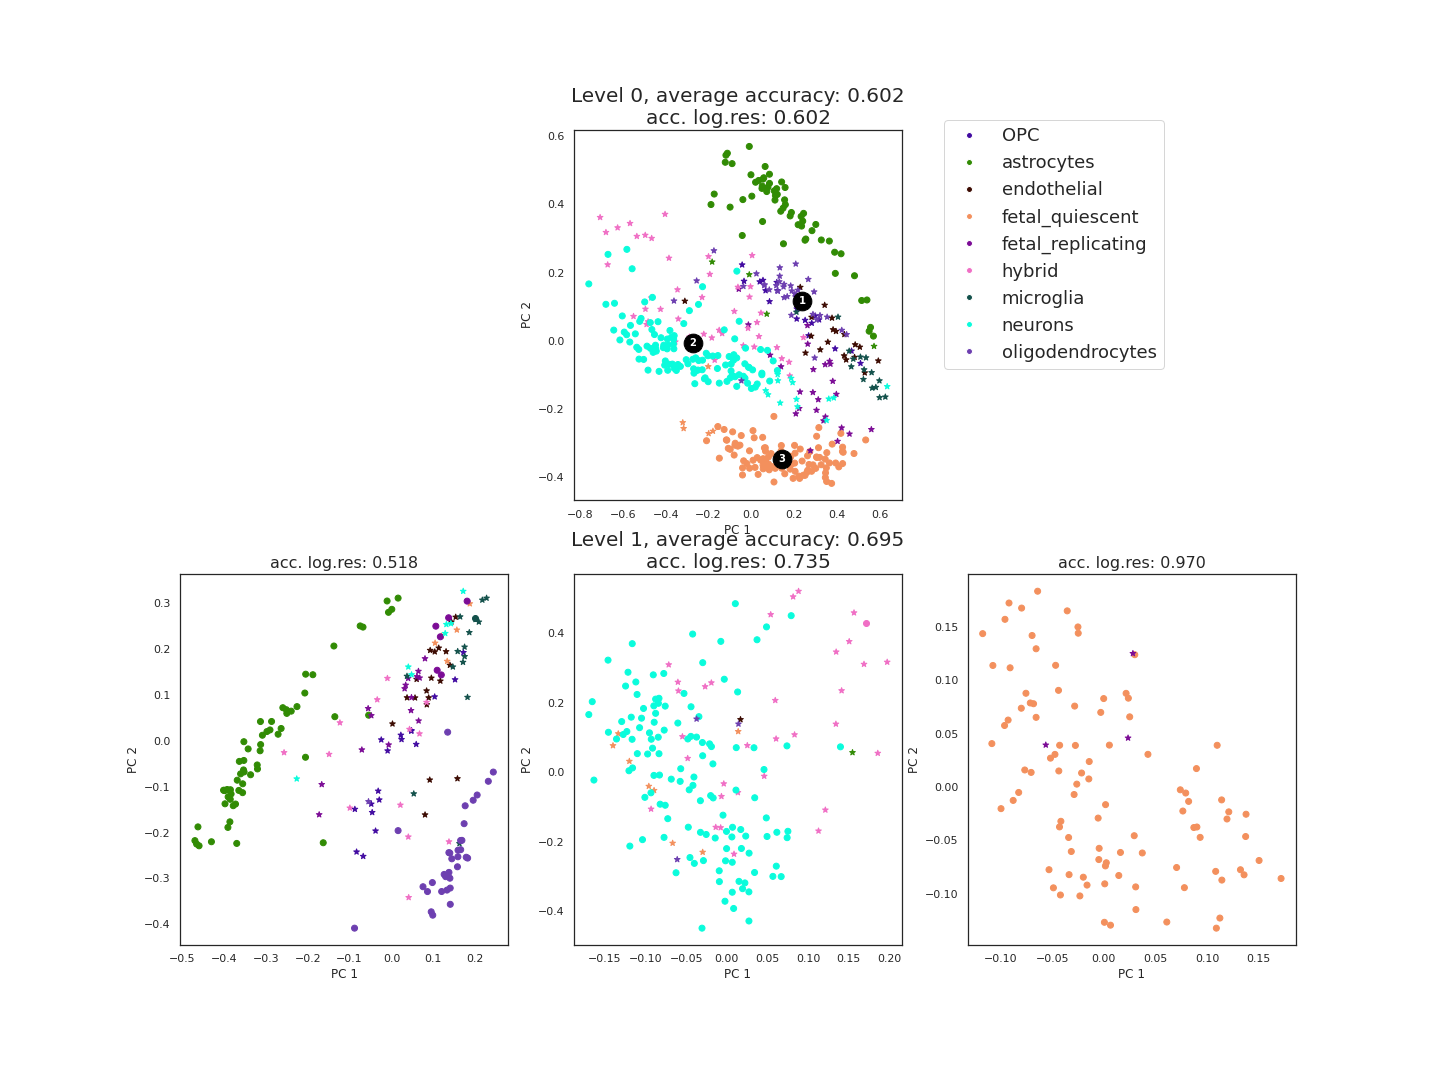
\includegraphics[width=\linewidth]{figs/Darmanis_tree_NUTS.png}
    \caption[The hmPPCAs analysis on the Darmanis data-set.]{\small \textbf{The hmPPCAs analysis on the Darmanis data-set.} \small NUTS was used for inference and one level was found. A maximum accuracy of $0.695$ was found at level $1$. The top-level PPCA achieved an accuracy of $0.602$. The clusters found within the top-level PPCA have been numbered. The colours indicate different cell types. Data-points that were predicted correctly by the logistic regression are plotted with dots, incorrect predictions are plotted with stars.}
    \label{fig:damanis_nuts}
\end{figure}

\begin{figure}
    \centering
    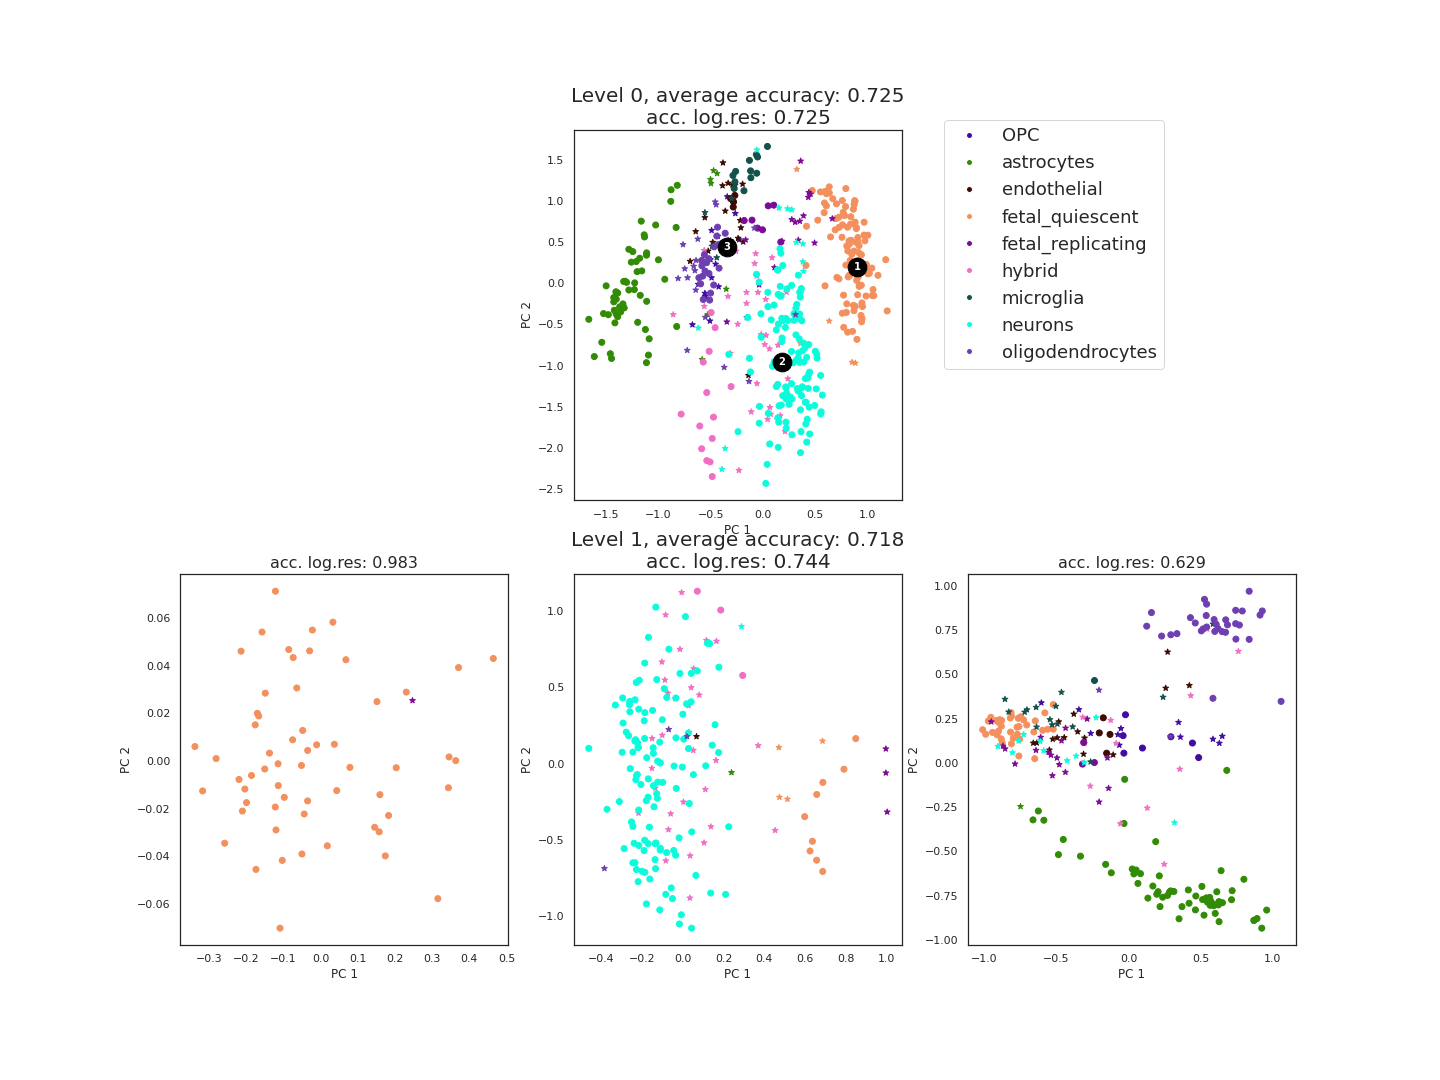
\includegraphics[width=\linewidth]{figs/Darmanis_tree_VB.png}
    \caption[The hmPPCAs analysis on the Darmanis data-set.]{\small \textbf{The hmPPCAs analysis on the Darmanis data-set.} \small VB was used for inference and one level was found. A maximum accuracy of $0.725$ was found at the top-level. The clusters found within the top-level PPCA have been numbered. The colours indicate different cell types. Data-points that were predicted correctly by the logistic regression are plotted with dots, incorrect predictions are plotted with stars.}
    \label{fig:darmanis_vb}
\end{figure}



% \textbf{Nestorowa data-set}\\

\begin{figure}
    \centering
    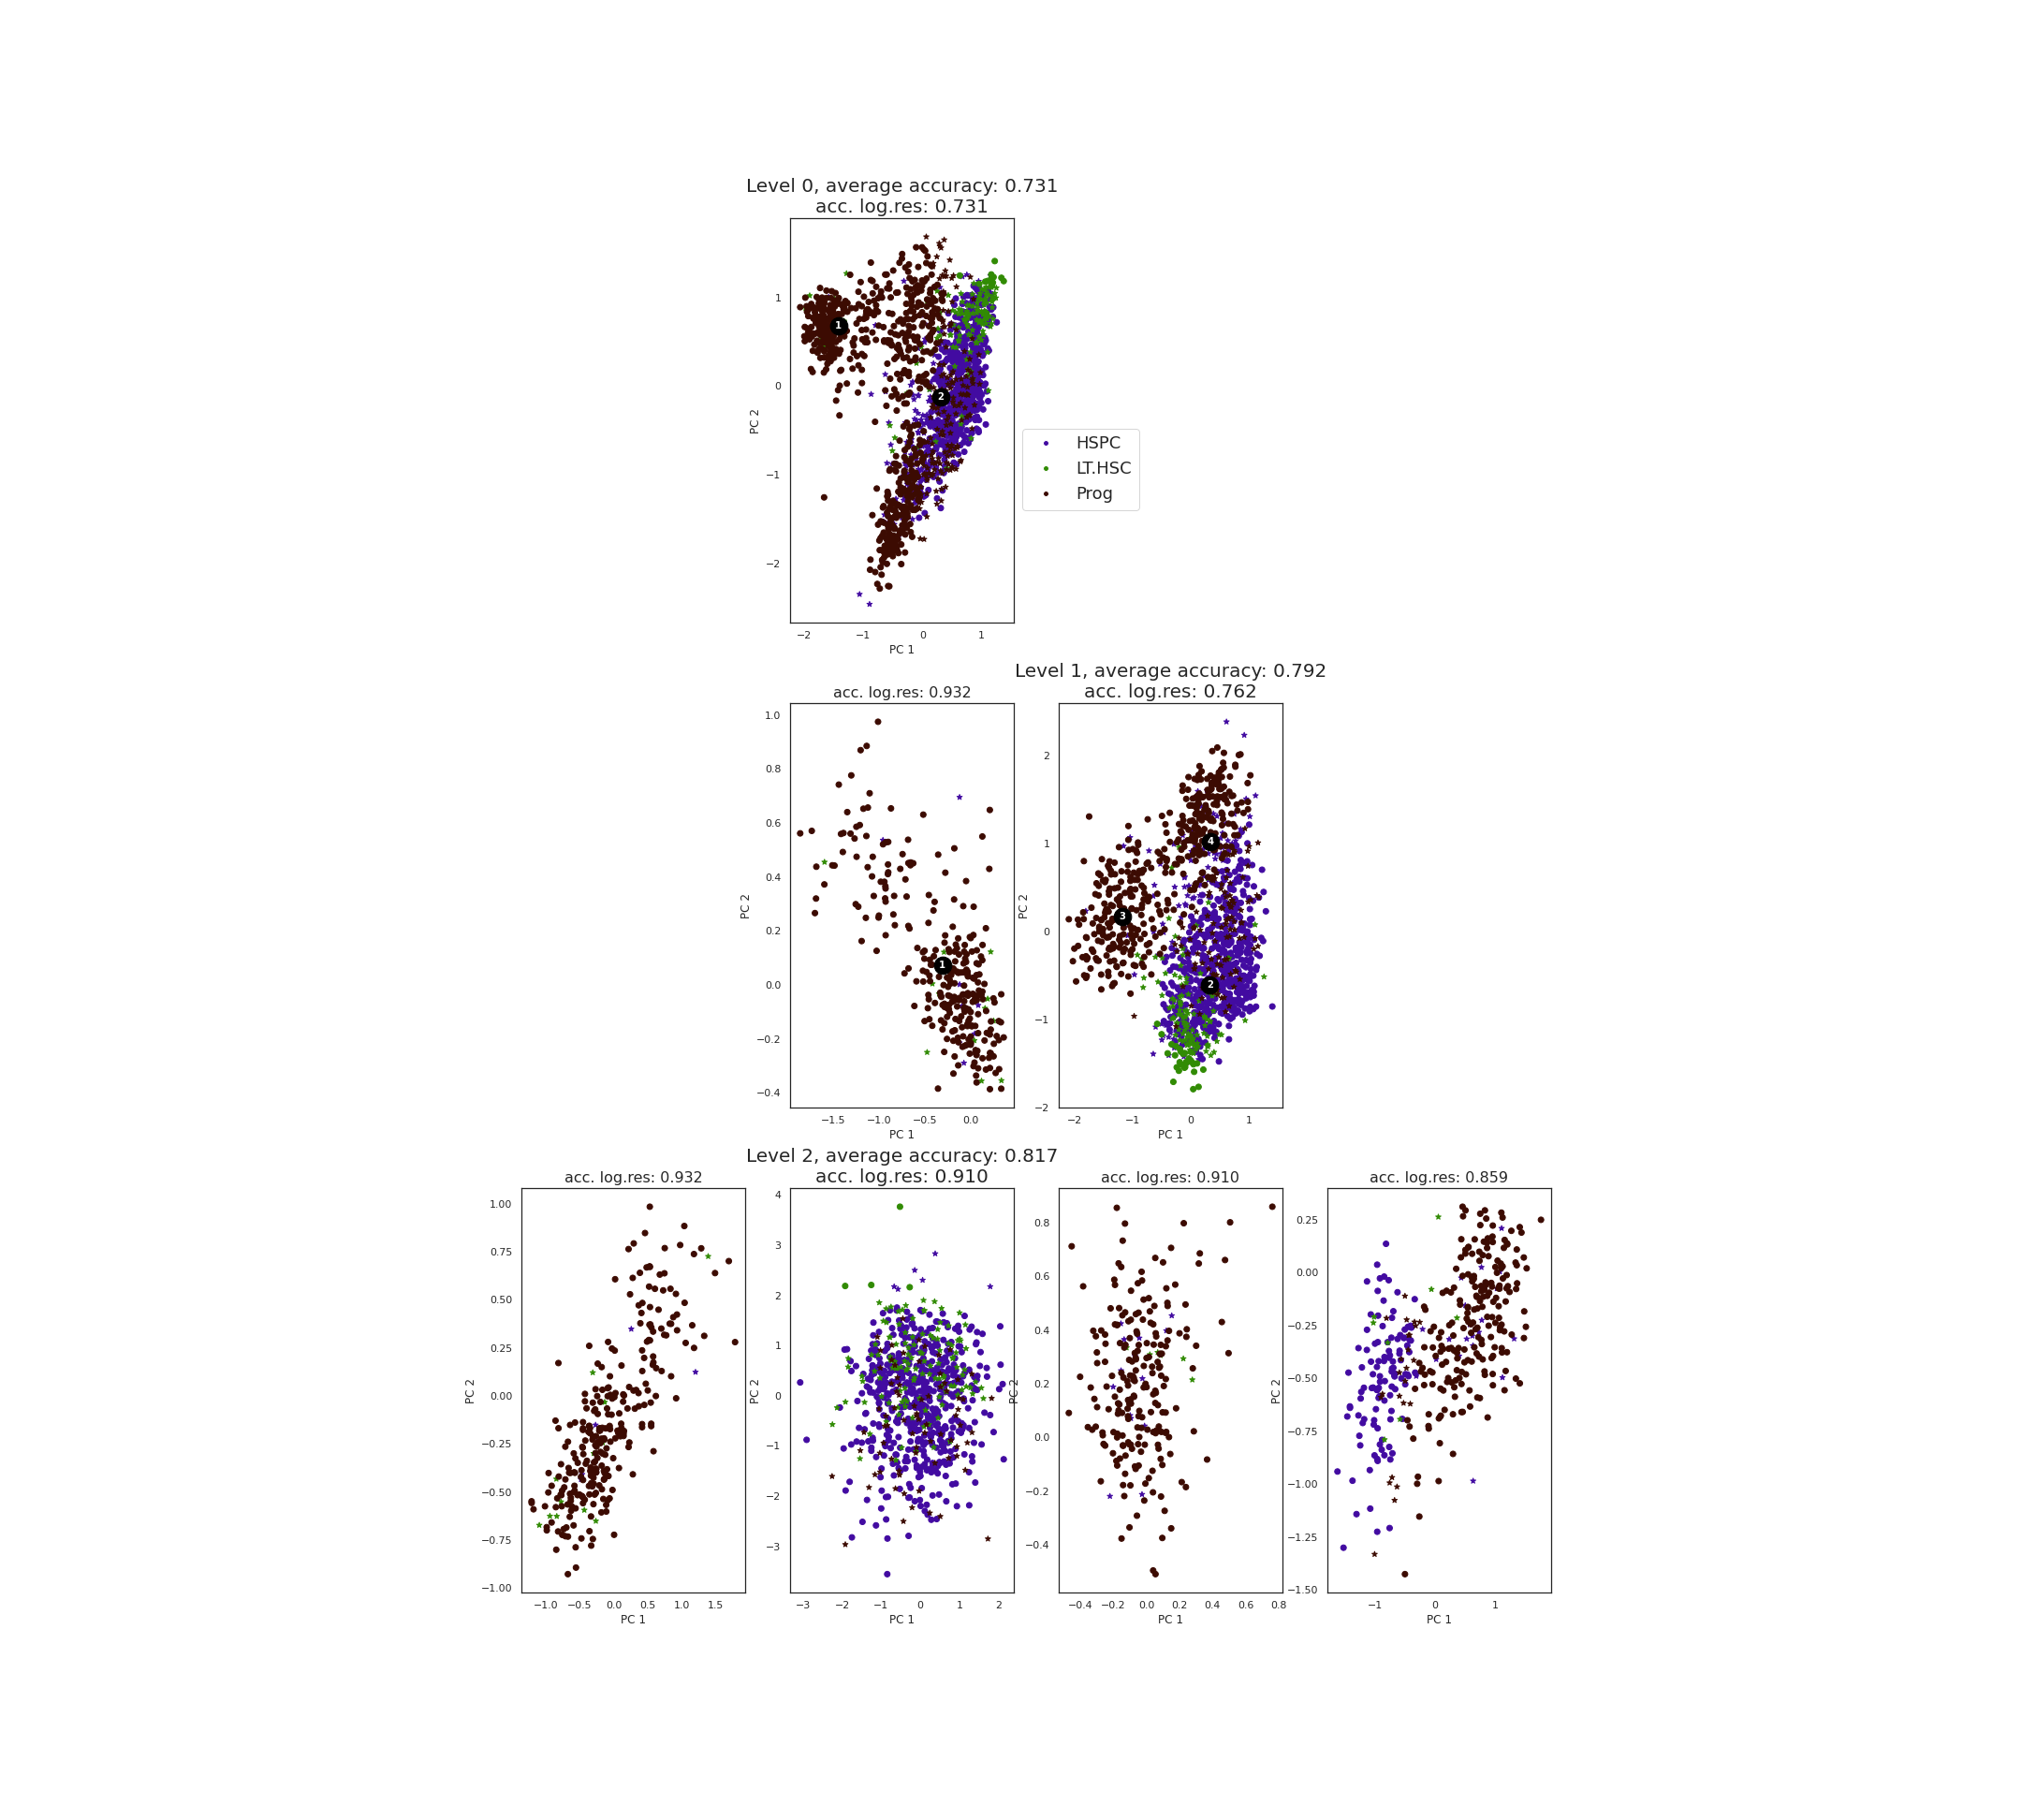
\includegraphics[width=0.95\linewidth]{figs/Nestorowa_tree_NUTS.png}
    \caption[The hmPPCAs analysis on the Nestorowa data-set.]{\small \textbf{The HmPPCAs analysis on the Nestorowa data-set.} \small NUTS was used as a sampling-method and five levels were found. A maximum accuracy of $0.817$ was found at level $2$. The top-level PPCA achieved an accuracy of $0.731$. The clusters found on each level have been numbered. The colours indicate different cell types. Data-points that were predicted correctly by the logistic regression are plotted with dots, incorrect predictions are plotted with stars.}
    \label{fig:nestorowa_nuts}
\end{figure}

\begin{figure}
    \centering
    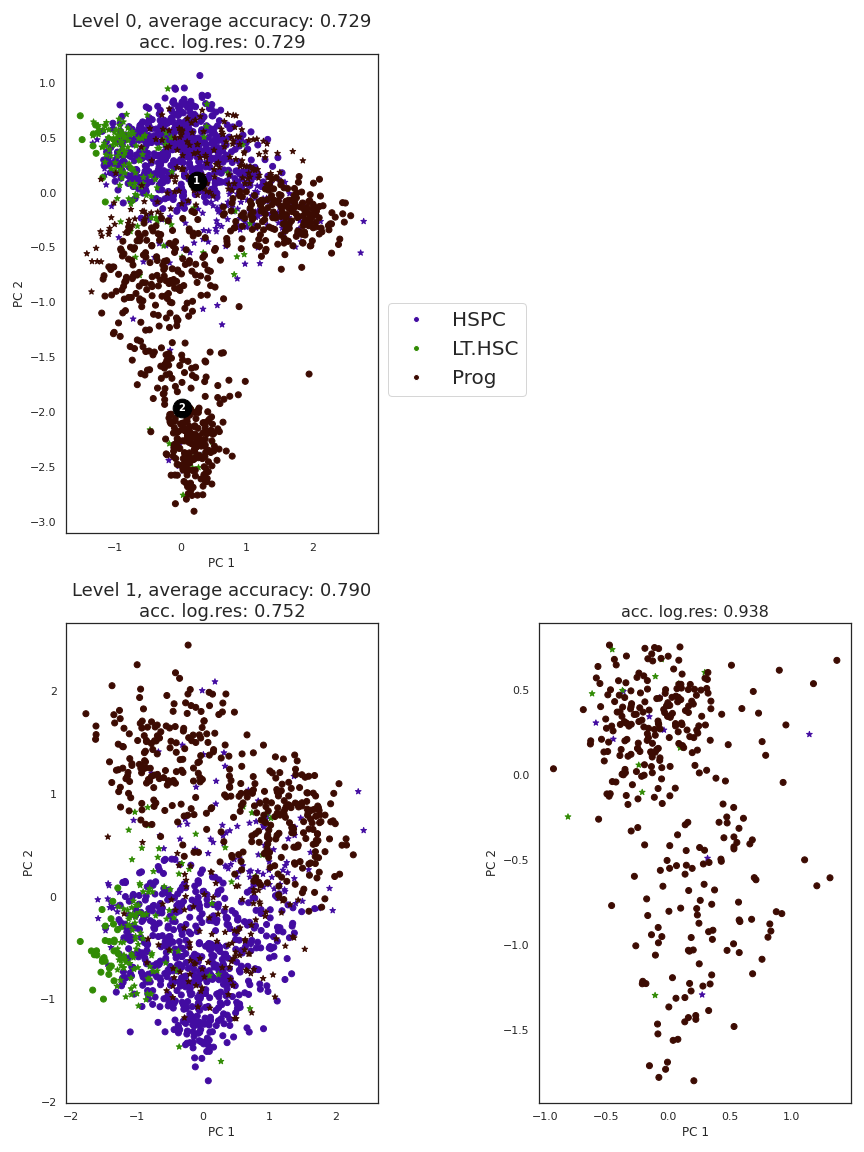
\includegraphics[width=.7\linewidth]{figs/Nestorowa_tree_VB.png}
    \caption[The hmPPCAs analysis on the Nestorowa data-set.]{\small \textbf{The HmPPCAs analysis on the Nestorowa data-set.} \small VB was used as a sampling-method and two levels were found. A maximum accuracy of $0.790$ was found at level $1$. The top-level PPCA achieved an accuracy of $0.729$. The clusters found within the top-level PPCA have been numbered. The colours indicate different cell types. Data-points that were predicted correctly by the logistic regression are plotted with dots, incorrect predictions are plotted with stars.}
    \label{fig:nestorowa_vb}
\end{figure}



\section{Computational cost}
Table \ref{tab:timetable} contains the computation times it took to infer the PPCA and MoPPCAs models on the Splatter data-sets. Each PPCA model was run only once at the top-level and its computation time is given. The MoPPCAs models were run repeatedly throughout the HmPPCAs models, so the average computation time of all MoPPCAs within the HmPPCAs is given instead. As expected, the PPCA models take less time to compute than the MoPPCAs models. This is the case for both NUTS and VB. We also see that VB takes considerably less time to infer solutions than NUTS for both the PPCA and the HmPPCAs models. The computational time goes up as the number of genes in the data-set rises, but more so when using NUTS than when using VB.

The time in seconds of the MoPPCAs models was also compared while taking the number of mixture components that the MoPPCAs models included into account. This was done for the Splatter data-sets and the results of this are shown in Figure \ref{fig:time_comps}. In some cases, a MoPPCAs model was initialized with a specific number of mixture components but ended up finding fewer mixture components. For this reason, both the number of initial mixture components and the number of found mixture components were taken into account separately. In both cases, there was no apparent relationship between the number of mixture components in a MoPPCAs model and the time it took to fit the model. Whereas sometimes the measured time became shorter when fewer mixture components were involved, this was the opposite for other cases, and in many cases, there was no effect to be observed at all.


\begin{table}
\setlength{\tabcolsep}{3pt}
    \caption[Computation times of PPCA and MoPPCAs models.]{\textbf{Computation times of PPCA and MoPPCAs models. In case multiple MoPPCAs were performed on a data-set within a HmPPCAs analyses, the average computation time of all MoPPCAs is reported.}}
    \centering
    \small
    \begin{tabular}{l|rrrrr|rrrrr}
          & \multicolumn{5}{r}{Splatter simple} & \multicolumn{5}{r}{Splatter complex}\\
          genes & 5 & 25 & 50 & 150 & 250 & 5 & 25 & 50 & 150 & 250\\
          \hline
        \makecell{PPCA\\(NUTS)} & 21.1 & 38.7 & 53.6 & 163.3 & 227.4 & 54.8 & 157.0 & 150.1 & 312.5 & 441.7\\
        \makecell{MoPPCAs\\(NUTS)} & 589.7 &  1313.2 & 1599.9 & 9266.6 & 10327.2 & 997.7 & 1945.1 & 2083.9 & 8409.1 & 17229.8\\
        \makecell{PPCA\\(VB)} & 2.8 & 4.4 & 5.3 & 11.3 & 14.0 & 7.0 & 16.1 & 11.3 & 20.8 & 14.3\\
        \makecell{MoPPCAs\\(VB)} & 31.5 & 48.6 & 101.1 & 276.6 & 208.3 & 11.5 & 28.3 & 48.7 & 210.7 & 104.9\\
    \end{tabular}
    % \medskip
    % \small
    % The average times in seconds to infer PPCA and MoPPCAs models when using NUTS and VB for all Splatter data-sets. NUTS takes more time to find a good fit of a model than ADVI. The computation time goes up when more genes are included into the set, but more so for NUTS than for ADVI.
    \label{tab:timetable}
\end{table}

\begin{figure}
    \centering
    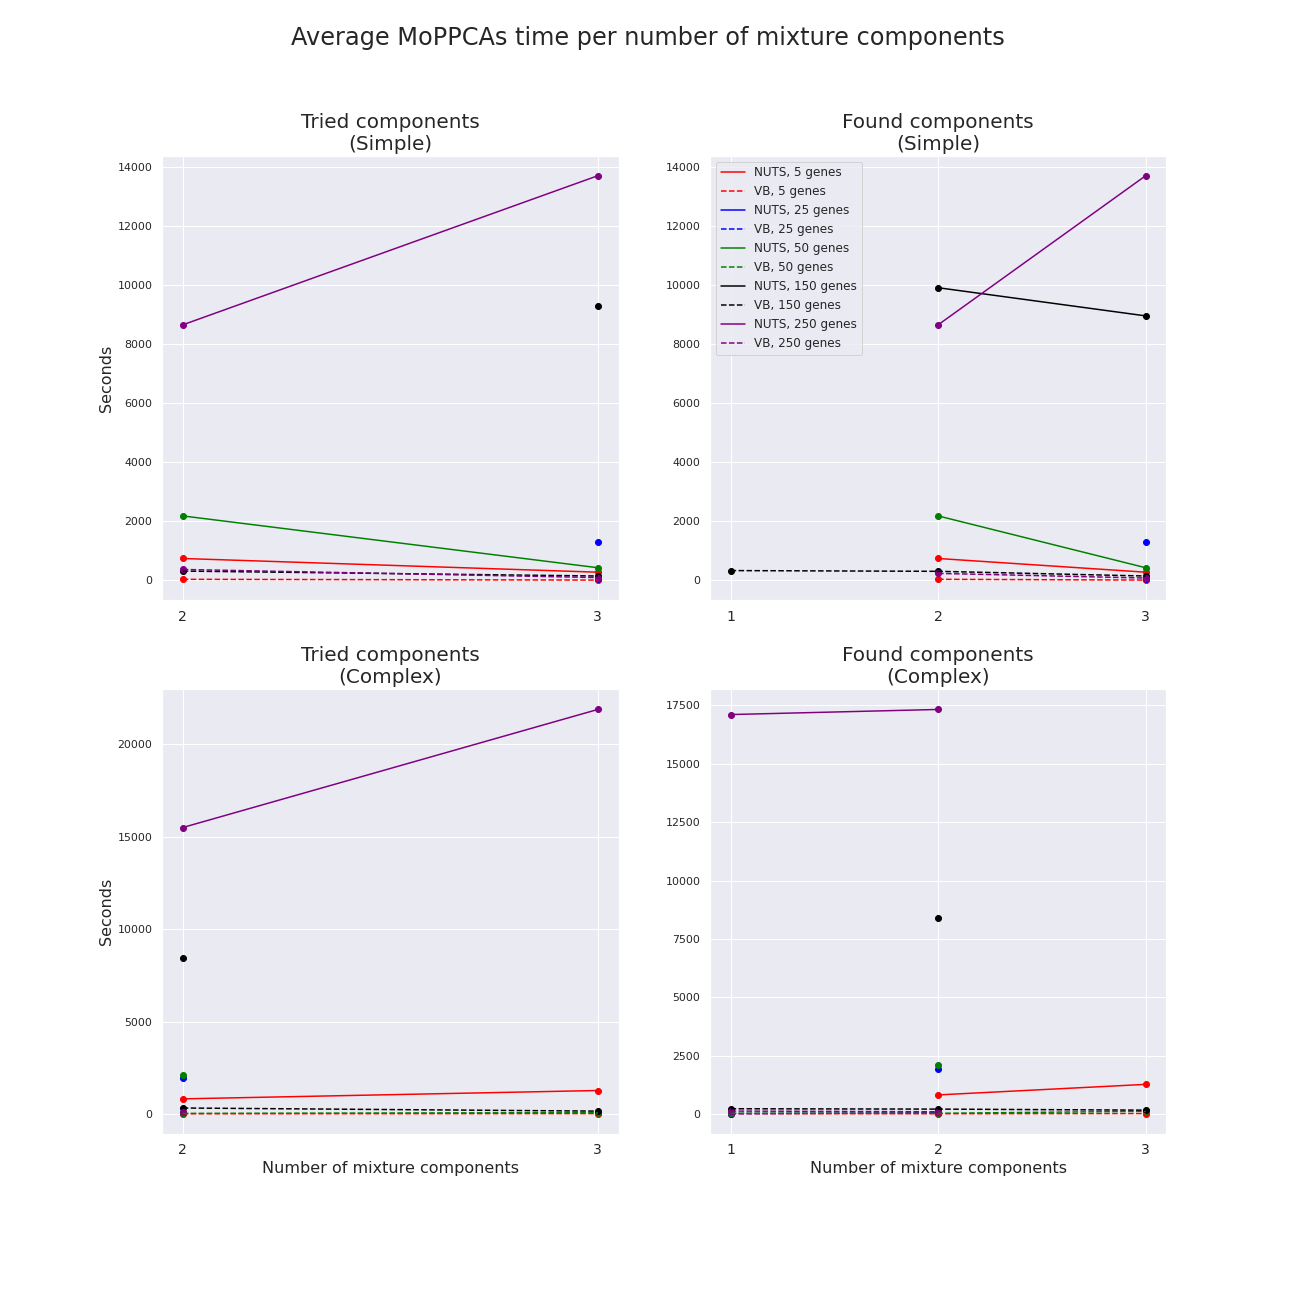
\includegraphics[width=\linewidth]{figs/time_mixture_comps.png}
    \caption[Average time to reach solution of MoPPCAs models in relation to their number of mixture components.]{\textbf{Average time to reach solution of MoPPCAs models in relation to their number of mixture components.}The two figures on the left show the (average) time is took for a MoPPCAs to be solved in relation to the number of mixture components that the model was suggested to find. The MoPPCAs models were always looking for either $2$ or $3$ mixture components. In some cases, less mixture components were found. The plots on the right relate the time to the number of mixture components that were found by the model, which may in some cases have been only $1$. The top two figures show this relation for the simple Splatter data-sets, the bottom two figures show this for the complex Splatter data-sets. In case of a dot that is not connected to another dot, no MoPPCAs model with a comparable number of mixture components has taken place in the HmPPCAs.}
    \label{fig:time_comps}
\end{figure}


% \subsection{Comparison NUTS and VB}

% \subsection{Our model in relation to other models}

% \section{Summary of all results}

\chapter{Discussion}\label{sec:discussion}
\lhead{\emph{Discussion}}
% \section{Short summary of results (subsection without title)}
We have evaluated the visualization performance of the HmPPCAs model on several simulated and two real scRNA-seq data-sets. We then compared these results with those obtained using PPCA, t-SNE and UMAP. We found that HmPPCAs was most of the time able to improve upon PPCA. Since a PPCA is performed on the top-level data-set as the first step of HmPPCAs, it is always included within the HmPPCAs. Therefore, it was impossible for the HmPPCAs to score lower than the PPCA model. We also found that, although HmPPCAs improved over PPCA, it was not as accurate as t-SNE and UMAP. Both these techniques were in general able to create plots that separated the different cell types better than HmPPCAs could. UMAP scored highest of the two, but t-SNE performed almost equally well.

We saw that the accuracy achieved by the HmPPCAs was comparable when using VB and NUTS as inference method. For the PPCA model negligibles difference were observed, except in the case of the Darmanis data-set, where NUTS performed relatively weak compared to all other methods. The HmPPCAs scored equally well when using NUTS as when using VB on many of the data-sets.
% On some of the data-sets, however, especially on the complex Splatter data-sets, VB scored higher. This was also true for the Darmanis data-set, where VB scored even higher with its top-level PPCA than the whole HmPPCAs using NUTS, although its score did not improve anymore after adding more levels of depth.

% The reason for the difference in performance between using NUTS and VB is not clear. The PPCA produced plots that achieved higher visualization scores when using NUTS. This implies that cell types were separated better in these plots. Therefore one would expect that this would lead to better clustering, and therefore also more accurate results on deeper levels. This was not true, as soon as deeper levels were initialized, VB achieved higher accuracy scores on the visualization assay.

NUTS and VB were also compared in terms of computation time till convergence. VB was always faster, for both the PPCA and HmPPCAs models. Not only did VB return results faster, but the computation time also increased less steeply when adding more genes, indicating that the method is more scalable.

% \section{Implications (subsection without title)}

The HmPPCAs model improved visualization performance over PPCA. In most cases, it was able to separate the different cell types better than just a single top-level PPCA.
It should be noted though, that here, the level with the highest accuracy was taken to evaluate the performance of a HmPPCAs model. The visualization scores of our HmPPCAs model are therefore an upper bound of the models.


Another point for discussion is that our MoPPCAs model was biased to find a relatively high value of $\sigma^2$ and a lower value of $\bm{W}$, as discussed in Section \ref{sec:prios}. An expected value of $\sigma^2$ was based on the spread of the clusters in the latent space. Also, constraints were forced upon the value of $\sigma^2$. To evaluate the effect of this approach, the value of $\sigma^2$ as found by the MoPPCAs model and the value found by the EM-algorithm for PPCA when performed on the separate clusters were compared with the values at which the constraints were set. Upon evaluation, the lower bound of $\sigma^2$ was (barely) high enough to include the value of $\sigma^2$ as found by PPCA, and the MoPPCAs solution for $\sigma^2$ was very similar to the PPCA solution. Still, future implementations of the MoPPCAs model in Stan should use priors and constraints for $\sigma^2$ which are based on their actual expectation. For example, according to Bishop \& Tipping \cite{bishop1998hierarchical}, the maximum likelihood estimator of $\sigma^2$ is given by $\sigma^2_{ML} = \frac{1}{d-2}\sum_{j=3}^d \lambda_j$, where $\lambda_j$ is the $j$th eigenvalue of the covariance matrix of the cluster. Basing the expectation $\sigma^2$ on this approach would be more correct.

It should also be noted that the number of iterations used for NUTS (300) was relatively low, in an attempt to save computational cost. When $\pm$250 iterations were used, Stan would give warnings that the samples might not have converged, so 300 iterations were used to avoid these warnings. Still, 300 iterations are on the low side. We do see reasonable results that were largely comparable with the VB results, but it is possible that better results could have been achieved when using a higher number of iterations.

Lastly, the parameters of our interest (e.g. the latent data-set $Z$ and the responsibility terms $\gamma_i^k$) were traceable. However, the factor loadings matrix $W$ is more difficult to find, because $W$ may undergo any arbitrary rotation. Therefore, if a researcher is interested in $W$, it may be better to use the EM algorithm. Alternatively, they could base the result on a single sample and not the mean of multiple samples.

Despite these shortcomings of our HmPPCAs implementation, HmPPCAs was able to provide more information about the local structure within clusters. A top-level PPCA might show some clusters, but the addition of hierarchy reveals structures within these clusters. For example, in Figure \ref{fig:simple_250_vb}, the top-level PPCA would suggest that there are only four observable clusters of cells in the data-set. When taking the purple-geen cluster apart and visualizing its data-points in its own latent space, it becomes clear that this cluster actually consists of two sub-clusters which could not be separated by a top-level PPCA. Visualizing the latent space of the data-set gives a good idea of which data-points could form a distinct group. The latent space of clusters within the data-set provides more information on these clusters than the PPCA representation when all data is taken into account. When encountering clusters while using linear dimensionality reduction techniques, it may, therefore, reward to perform separate analyses on the clusters within the data-set.

Additionally, it is noteworthy that HmPPCAs does not necessarily separate cell types, but specifically cluster structures in the data. Figure \ref{fig:nestorowa_nuts} shows how one group, the progenitor cells, shows different clusters. Each of those clusters is taken separately for further analysis, even though they belong to the same group of cells. This is not necessarily a bad thing and it is possible that there are differences to be found in the cells belonging to this type. Therefore, it could be the case that even subsets of the data-set that belong to the same type of cells need different analyses in terms of dimensionality reduction.

When comparing the HmPPCAs with UMAP and t-SNE however, it did not reach their visualization performance quite yet. It seems therefore that UMAP and t-SNE are non-linear approaches that are better at separating groups within the data than PPCA, even when extended to HmPPCAs. This might be due to the automatic clustering since the interactive EM implementation of HmPPCAs has been found to improve on t-SNE \cite{philipsthesis}. They may therefore have the advantage in the visualization assay that was performed.

% However, HmPPCAs has its own advantages, as it gives a more accurate representation of the real structure of the data-set, even though this does not necessarily separate groups within the data structure.

% \section{Future research (subsection without title)}

% \section{Final conclusion(s) (subsection without title)}
All in all, extending PPCA to a hierarchical model is a good way to obtain more insight into the local structure of the data-set. It might not be as good as UMAP or t-SNE to separate different structures within the data, but it is a valuable extension to linear dimensionality reduction techniques. Also, it seems that VB did not perform significantly worse than NUTS and possibly even better on some models. VB also took less time to converge and showed better scalability when adding more genes. The ADVI algorithm has therefore proven to be of great value when using Stan.


%----------------------------------------------------------------------------------------
%	THESIS CONTENT - APPENDICES
%----------------------------------------------------------------------------------------

\addtocontents{toc}{\vspace{2em}} % Add a gap in the Contents, for aesthetics

%\appendix % Cue to tell LaTeX that the following 'chapters' are Appendices

% Include the appendices of the thesis as separate files from the Appendices folder
% Uncomment the lines as you write the Appendices

\appendix
% \appendix
\section{Symbols and their meanings}
\printunsrtglossary[type=symbols,style=long]

\section{Gaussian distribution}
\subsection{Converting probability to its log-probability}\label{AP:log_prob}
\begin{equation}\label{eq:ap_logprob}
\begin{split}
    \ln p(\textbf{x}^n_1 | \mu, \sigma^2) &= \prod_{i=1}^{n}{\mathcal{N}(x_i|\mu, \sigma^2)}\\
    \ln p(\textbf{x}^n_1 | \mu, \sigma^2) &= \ln \prod_{i=1}^{n}\frac{1}{(2 \pi \sigma ^2)^{\frac{1}{2}}} e^{- \frac{1}{2\sigma ^2}(x_i - \mu)^2}\\
    \ln p(\textbf{x}^n_1 | \mu, \sigma^2) &= \sum_{i=1}^{n} \ln \frac{1}{(2 \pi \sigma ^2)^{\frac{1}{2}}} e^{- \frac{1}{2\sigma ^2}(x_i - \mu)^2}\\
    \ln p(\textbf{x}^n_1 | \mu, \sigma^2) &= \sum_{i=1}^{n} \ln \frac{1}{(2 \pi \sigma ^2)^{\frac{1}{2}}} + \ln e^{- \frac{1}{2\sigma ^2}(x_i - \mu)^2}\\
    \ln p(\textbf{x}^n_1 | \mu, \sigma^2) &= \sum_{i=1}^{n} -\frac{1}{2} \ln (2 \pi \sigma ^2) - \frac{1}{2\sigma ^2}(x_i - \mu)^2\\
    \ln p(\textbf{x}^n_1 | \mu, \sigma^2) &= \sum_{i=1}^{n} -\frac{1}{2} \ln (2 \pi \sigma ^2) - \frac{1}{2\sigma ^2}(x_i - \mu)^2\\
    \ln p(\textbf{x}^n_1 | \mu, \sigma^2) &= -\frac{n}{2} \ln 2 \pi -\frac{n}{2} \ln \sigma ^2 - \sum_{i=1}^{n} \frac{1}{2\sigma ^2}(x_i - \mu)^2\\
\end{split}
\end{equation}

\subsection{Maximum likelihood for $\mu$}\label{AP:mu_ML}
\begin{equation}\label{eq:ap_derivative_mu}
\begin{split}
    \frac{\partial }{\partial \mu } \big( - \frac{n}{2} \ln{2 \pi} - \frac{n}{2} \ln{\sigma ^2} - \sum_{i=1}^{n} \frac{1}{2\sigma ^2}(x_i - \mu_{ML})^2 \big) &= 0\\
    \frac{\partial}{\partial \mu} \big( - \sum_{i=1}^{n} \frac{1}{2\sigma ^2}(x_i - \mu_{ML})^2 \big) &= 0\\
    - \sum_{i=1}^{n} \frac{1}{2\sigma ^2}(-2 x_i + 2 \mu_{ML}) &= 0\\
    \sum_{i=1}^{n} \frac{2 x_i}{2\sigma ^2} &= \sum_{i=1}^{n} \frac{2 \mu_{ML}}{2\sigma ^2}\\
    \sum_{i=1}^{n} x_i &= n \mu_{ML}\\
    \frac{1}{n} \sum_{i=1}^{n} x_i &= \mu_{ML}\\
\end{split}
\end{equation}

\subsection{Maximum likelihood for $\sigma^2$}\label{AP:s2_ML}

\begin{equation}\label{eq:ap_derivative_sigma}
\begin{split}
    \frac{\partial }{\partial \sigma^2 } \big( - \frac{n}{2} \ln{2 \pi} - \frac{n}{2} \ln{\sigma^2_{ML}} - \sum_{i=1}^{n} \frac{1}{2\sigma^2_{ML}}(x_i - \mu_{ML})^2 \big) &= 0\\
    \frac{\partial}{\partial \sigma^2} \big( - \frac{n}{2} \ln{\sigma^2_{ML}}  - \sum_{i=1}^{n} \frac{1}{2\sigma^2_{ML}}(x_i - \mu_{ML})^2 \big) &= 0\\
    \frac{n}{2\sigma^2_{ML}} - \sum_{i=1}^{n} \frac{1}{2{\sigma^2_{ML}}^2}(x_i - \mu_{ML})^2 &= 0\\
    n\sigma^2_{ML} - \sum_{i=1}^{n} (x_i - \mu_{ML})^2 &= 0\\
    \frac{1}{n} \sum_{i=1}^{n} (x_i - \mu_{ML})^2 &= \sigma^2_{ML}\\
\end{split}
\end{equation}


% \chapter{Symbols}
\printunsrtglossary[type=symbols,style=long]
\chapter{Fitting a model to the data}\label{ap:prob_theory}

% \subsubsection{Foundational knowledge on probability theory}
\section{The Gaussian distribution}

\begin{wrapfigure}{r}{.5\textwidth}
    \centering
    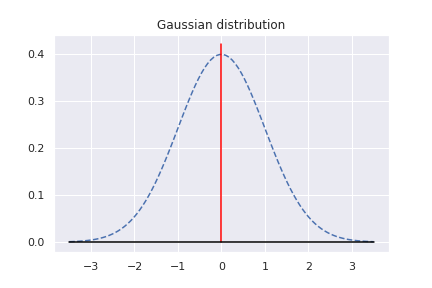
\includegraphics[width=\linewidth]{figs/normal_dist.png}
    \caption[The probability density function for a standard Gaussian or normal distribution]{\small \textbf{The probability density function for a standard Gaussian or normal distribution.}}
    \label{fig:gauss}
\end{wrapfigure}


Let's say we observe a random variable $x$. Random variables have a value that is not predetermined, but sometimes we know how the probability of drawing a random value is depending on that value. When the random number can assume any number (i.e. not only discrete integers), then a probability density function gives the probability density for the support of $\mathcal{X}$ (i.e. the values that $x$ can assume). One well-known example of such a probability density function is the Gaussian distribution. It is defined by \ref{eq:gauss}.

\begin{equation}\label{eq:gauss}
    \mathcal{N}(x|\mu, \sigma^2)=\frac{1}{(2 \pi \sigma ^2)^{\frac{1}{2}}} e^{- \frac{1}{2\sigma ^2}(x - \mu)^2}
\end{equation}

The mean $\mu$ is the value around which all drawn samples are centered, and the standard deviation $\sigma$ tells us how far the drawn samples are spread out from this point. Drawing a sample of $n$ independent and identically distributed (i.i.d.) data points from the Gaussian distribution given its mean and variance is done with a probability of the product of the probabilities of drawing the individual data points (see \ref{eq:gauss_prod}, where $\textbf{x}^n$ is a set of $n$ data points).

\begin{equation}\label{eq:gauss_prod}
    p(\textbf{x}^n | \mu, \sigma^2) = \prod_{i=1}^{n}{\mathcal{N}(x_i|\mu, \sigma^2)}
\end{equation}

Sometimes, we deal with multivariate random variables. In this case, every data-point $\bm{x}_i$ and the mean $\bm{\mu}$ are $d$-dimensional vectors and the covariance matrix $\bm{\Sigma}$ is a $d \times d$ matrix noting the co-variances among all dimensions. In this case, $\textbf{X}$ is a matrix containing $n$ rows $\textbf{x}_i$ of length $d$ for each data point. In this case, $\bm{\mu}^d$ is a $d$-dimensional vector where $\mu_j$ notes the mean of the $j$th variable. The covariances between all variables are given by positive semi-definite matrix $\bm{\Sigma}$, where $\bm{\Sigma}_{i,j}$ describes the covariance between the $i^\text{th}$ and $j^\text{th}$ variable. Note that $\bm{\Sigma}$ is symmetric, as a property of covariance, and that $\bm{\Sigma}_{i,i}=cov(x_i,x_i) = var(x_i)$. For a set of independent variables, $\bm{\Sigma}$ is a diagonal matrix, since the $cov(x_i,x_j)$ is $0$ when $i\neq i$. In a multivariate setting, the Gaussian distribution takes the form of \ref{eq:gaus_mn}.

\begin{equation}\label{eq:gaus_mn}
    \mathcal{N}(\textbf{x}|\bm{\mu}, \bm{\Sigma})=\frac{1}{(2 \pi)^{\frac{m}{2}}}\frac{1}{|\bm{\Sigma}|^{\frac{1}{2}}} e^{- \frac{1}{2}(\textbf{x} - \bm{\mu})^T \bm{\Sigma}^{-1}(\textbf{x} - \bm{\mu})}
\end{equation}

\section{Likelihood and the posterior}
 Let's say we have the probability density function of $\bm{x}$, $p(\bm{x}|\theta)$, where $\theta$ holds the parameters of the distribution of $p(x)$ (e.g. in this case $\theta = (\mu, \sigma^2)$). Apart from deriving the probability of drawing a value from a given distribution and its parameters, we can also derive the likelihood of the parameters of the distribution being certain values given only the observed data. A noteworthy difference between the probability and the likelihood is that the probability necessarily sums up to $1$ when integrated over the support of $\mathcal{X}$, but the likelihood does not when integrating over the parameter space of $\theta$. The likelihood is given by $\mathcal{L}(\theta|\bm{x}) = p(\bm{x}|\theta)$. This likelihood is often given by its logarithm, known as the log-likelihood. On the one hand, this makes mathematical manipulations with Gaussian distributions a lot easier. On the other hand, the log function converts very small numbers to larger ones, which helps to avoid numerical underflow on electronic devices. Converting the likelihood function of \ref{eq:gauss_prod} to a corresponding log-likelihood function results in \ref{eq:logprob} (derivation in \ref{AP:log_prob}).

\begin{equation}\label{eq:logprob}
    \ln \mathcal{L}(\mu, \sigma^2 | \bm{x}) = \ln p(\textbf{x} | \mu, \sigma^2) = -\frac{n}{2} \ln 2 \pi -\frac{n}{2} \ln \sigma ^2 - \frac{1}{2\sigma ^2} \sum_{i=1}^{n} (x_i - \mu)^2
\end{equation}

Using the log-likelihood has two advantages: It makes mathematical manipulations to the distribution fairly easy and it avoids numerical underflow errors by converting very small numbers to larger ones. Since the log function is monotonically increasing, the maximum of the likelihood function s found for the same value as the maximum of the log-likelihood.

 The likelihood, however, is not the same as the probability that $\theta$ is responsible for generating data $\bm{x}$. According to Bayes' theorem, $p(A|B) = \frac{p(B|A) p(A)}{p(B)}$, and therefore the likelihood of parameters $\theta$ being responsible for observed data $\bm{x}$ is given by $p(\theta|\bm{x}) = \frac{p(\bm{x}|\theta) p(\theta)}{p(\bm{x})}$. In this construction, the first term $P(\bm{x}|\theta)$ is the likelihood and the second term $p(\theta)$ is known as the prior. The prior takes the distribution of the parameters into account. Since the divisor is not dependent on $\theta$, $p(\bm{x}|\theta) p(\theta) \propto p(\theta|\bm{x})$ so that the product of the prior and likelihood determines the probability of $\theta$ being a certain value given the data. The last term, $p(\bm{x})$, is known as the evidence. It normalizes the probability, so that the posterior integrated over the parameter-space $\theta$ sums to $1$. When estimating $\theta$ given $\bm{x}$, a point estimate is given by $\text{argmax}_\theta p(\theta|\bm{x})$.
 
 Often, a prior distribution of $\theta$ is unknown or assumed to be of a uniform shape. In this case, the prior $p(\theta$ is a constant that is non-dependent on $\theta$ and $ p(\theta|\bm{x}) \propto p(\bm{x}|\theta)$. The point estimate for $\theta$ is then $\text{argmax}_\theta p(\bm{x}|\theta)$, known as the maximum likelihood (\textbf{ML}) estimate. This estimate can be found by taking the derivative of $\mathcal{L}(\theta|\bm{x})$ and setting it to $0$. For example, the ML estimates for $\mu$ is given by $\mu_{ML} = \frac{1}{n} \sum_{i=1}^{n} x_i$ and for $\sigma^2$ by $\sigma^2_{ML} = \frac{1}{n} \sum_{i=1}^{n} (x_i - \mu_{ML})^2$ (see \ref{AP:mu_ML} and \ref{AP:s2_ML}).\\

\section{Gaussian mixture models and EM}\label{app:gmm_em}
Now imagine that our data-set consists of different `groups' that all have their own mean and covariance matrix. For example, we may have a data-set with several cell-types, and every cell-type demonstrates their own pattern of gene expression. If our data-set consists of $K$ different Gaussians, then we have a Gaussian mixture model (\textbf{GMM}), of which the probability density function is denoted by \ref{eq:mm}.

\begin{equation}\label{eq:mm}
    p(x) = \sum_{k=1}^K \pi_k \mathcal{N}(x|\bm{\mu}_k, \bm{\Sigma}_k)
\end{equation}

In this example, $\bm{\mu}_k$ and $\bm{\Sigma}_k$ give the means and covariance matrix of each distribution $k$ and $\pi_k$ is the proportion in which mixture component $k$ is responsible for generating the data-set, such that $\sum^K_{k=1}\pi_k = 1$ and $\pi_k\geq0$ for all $k$.
 Finding the set of parameters $\theta = (\pi, \bm{\mu}, \bm{\Sigma})$ in this scenario is not as straight forward as the ML approach we saw earlier. To approximate $\theta$ for this model, we can use an iterative expectation-maximization (\textbf{EM}) algorithm. An EM-algorithm consist of two steps:
 
 \begin{itemize}
     \item In the Expectation-step, the expected log-likelihood function of the complete data-set (observed data and missing parameters) is estimated from their joint probabilities.
     \item In the maximization step, the parameters $\theta$ are maximized based on the estimated log-likelihood.
 \end{itemize}

 After we have chosen some arbitrary initial values for $\bm{\mu}_k$, $\bm{\Sigma}_k$ and $\pi_k$, we start with the E-step. In the E-step of our algorithm, we try to find the complete log-likelihood function. Let $\bm{z}_i$ denote which mixture component has generated data-point $i$. Then the complete likelihood function is given by \ref{eq:gmm_llh}, where $\mathbb{I}[z_i=j]$ evaluates to $1$ if true and $0$ otherwise. 

\begin{equation}\label{eq:gmm_llh}
    \mathcal{L}(\bm{X}|\theta, \bm{z}) = \prod^n_{i=1} \prod^K_{j=1} \mathcal{N}(\bm{x}_i|\theta_k)^{\mathbb{I}[z_i=j]}
\end{equation}

Now, $\bm{z}$ (i.e. which data-points were generated by which distribution) is unknown, but instead of $\mathbb{I}[z_i=j]$, we could use the probability $p(z_i=j)$. We know that $p(\bm{x}_i|z_i=j) = \mathcal{N}(\bm{x}_i|\bm{\mu}_j, \bm{\Sigma}_j)$ and therefore, we can compute the posterior $p(z_i=j|\bm{X})$ according to Bayes' theorem as done in \ref{eq:mix_prob}.

\begin{equation}\label{eq:mix_prob}
    p(z_k=j|\textbf{x}_i)
    =\frac{p(z_i=1) p(\textbf{x}_i|z_i=j)}{\sum^K_{k=1}p(z_i=k)p(\textbf{x}_i|z_i=k)}
    = \frac{\pi_j\mathcal{N}(\textbf{x}_i|\bm{\mu}_j, \bm{\Sigma}_j)}{\sum_{k=1}^K\pi_k\mathcal{N}(\textbf{x}_i|\bm{\mu}_k, \bm{\Sigma}_k)} 
\end{equation}

In the literature, the posterior probability is often denoted as $\gamma(z_{k,i}) = p(z_i=k|\bm{X})$.
With this, we can compute the expected complete log-likelihood $\ln \mathcal{L}(\theta|\bm{X}) = \sum^n_{i=1} \sum^K_{j=1} p(z_i=j) \ln \mathcal{N}(\bm{x}_i|\theta_k)$. In the M-step, we utilise this expected log likelihood to calculate ML-estimates for the mean $\bm{\mu}_k$, covariance-matrix $\bm{\Sigma}_k$ and mixing coefficient $\pi_k$ of each distribution $k$.

We start off with the mean of each distribution $k$. Setting the derivative with respect to $\bm{\mu}_k$ to $0$ shows that the ML estimate is simply given as the weighted average of all points belonging to distribution $k$ (\ref{eq:mm_mu}.

\begin{equation}\label{eq:mm_mu}
    \bm{\mu}_k = \frac{1}{\sum^n_{i=1} \gamma(z_{k,i})} \sum^n_{i=1} \gamma(z_{k,i}) \textbf{x}^m_i
\end{equation}

Similarly, the variance is computed as the weighted variance.

\begin{equation}\label{eq:mm_var}
    \bm{\Sigma}_k = \frac{1}{\sum^n_{i=1} \gamma(z_{k,i})} \sum^n_{i=1} \gamma(z_{k,i}) (\textbf{x}^m_i-\bm{\mu}_k)(\textbf{x}^m_i-\bm{\mu}_k)^T
\end{equation}

Finally, $\pi_k$ is obtained as the average of the individual probabilities with which points belong to distribution $k$.

\begin{equation}\label{eq:mm_mix}
    \pi_k = \frac{\sum^n_{i=1}{} \gamma(z_{k,i})}{n}
\end{equation}

Having obtained new values for all relevant parameters, we return to the E-step and obtain new posterior probabilities. The process is repeated until a converged state is reached.\\

\chapter{Gaussian distribution}
\section{Converting probability to its log-probability}\label{AP:log_prob}
\begin{equation}\label{eq:ap_logprob}
\begin{split}
    \ln p(\textbf{x}^n_1 | \mu, \sigma^2) &= \prod_{i=1}^{n}{\mathcal{N}(x_i|\mu, \sigma^2)}\\
    \ln p(\textbf{x}^n_1 | \mu, \sigma^2) &= \ln \prod_{i=1}^{n}\frac{1}{(2 \pi \sigma ^2)^{\frac{1}{2}}} e^{- \frac{1}{2\sigma ^2}(x_i - \mu)^2}\\
    \ln p(\textbf{x}^n_1 | \mu, \sigma^2) &= \sum_{i=1}^{n} \ln \frac{1}{(2 \pi \sigma ^2)^{\frac{1}{2}}} e^{- \frac{1}{2\sigma ^2}(x_i - \mu)^2}\\
    \ln p(\textbf{x}^n_1 | \mu, \sigma^2) &= \sum_{i=1}^{n} \ln \frac{1}{(2 \pi \sigma ^2)^{\frac{1}{2}}} + \ln e^{- \frac{1}{2\sigma ^2}(x_i - \mu)^2}\\
    \ln p(\textbf{x}^n_1 | \mu, \sigma^2) &= \sum_{i=1}^{n} -\frac{1}{2} \ln (2 \pi \sigma ^2) - \frac{1}{2\sigma ^2}(x_i - \mu)^2\\
    \ln p(\textbf{x}^n_1 | \mu, \sigma^2) &= \sum_{i=1}^{n} -\frac{1}{2} \ln (2 \pi \sigma ^2) - \frac{1}{2\sigma ^2}(x_i - \mu)^2\\
    \ln p(\textbf{x}^n_1 | \mu, \sigma^2) &= -\frac{n}{2} \ln 2 \pi -\frac{n}{2} \ln \sigma ^2 - \sum_{i=1}^{n} \frac{1}{2\sigma ^2}(x_i - \mu)^2\\
\end{split}
\end{equation}

\section{Maximum likelihood for \texorpdfstring{$\mu$}{the mean}}\label{AP:mu_ML}
\begin{equation}\label{eq:ap_derivative_mu}
\begin{split}
    \frac{\partial }{\partial \mu } \big( - \frac{n}{2} \ln{2 \pi} - \frac{n}{2} \ln{\sigma ^2} - \sum_{i=1}^{n} \frac{1}{2\sigma ^2}(x_i - \mu_{ML})^2 \big) &= 0\\
    \frac{\partial}{\partial \mu} \big( - \sum_{i=1}^{n} \frac{1}{2\sigma ^2}(x_i - \mu_{ML})^2 \big) &= 0\\
    - \sum_{i=1}^{n} \frac{1}{2\sigma ^2}(-2 x_i + 2 \mu_{ML}) &= 0\\
    \sum_{i=1}^{n} \frac{2 x_i}{2\sigma ^2} &= \sum_{i=1}^{n} \frac{2 \mu_{ML}}{2\sigma ^2}\\
    \sum_{i=1}^{n} x_i &= n \mu_{ML}\\
    \frac{1}{n} \sum_{i=1}^{n} x_i &= \mu_{ML}\\
\end{split}
\end{equation}

\section{Maximum likelihood for \texorpdfstring{$\sigma^2$}{the standard deviation}}\label{AP:s2_ML}

\begin{equation}\label{eq:ap_derivative_sigma}
\begin{split}
    \frac{\partial }{\partial \sigma^2 } \big( - \frac{n}{2} \ln{2 \pi} - \frac{n}{2} \ln{\sigma^2_{ML}} - \sum_{i=1}^{n} \frac{1}{2\sigma^2_{ML}}(x_i - \mu_{ML})^2 \big) &= 0\\
    \frac{\partial}{\partial \sigma^2} \big( - \frac{n}{2} \ln{\sigma^2_{ML}}  - \sum_{i=1}^{n} \frac{1}{2\sigma^2_{ML}}(x_i - \mu_{ML})^2 \big) &= 0\\
    \frac{n}{2\sigma^2_{ML}} - \sum_{i=1}^{n} \frac{1}{2{\sigma^2_{ML}}^2}(x_i - \mu_{ML})^2 &= 0\\
    n\sigma^2_{ML} - \sum_{i=1}^{n} (x_i - \mu_{ML})^2 &= 0\\
    \frac{1}{n} \sum_{i=1}^{n} (x_i - \mu_{ML})^2 &= \sigma^2_{ML}\\
\end{split}
\end{equation}

\chapter{PPCA model defined in Stan}\label{AP:ppca_stan}

This below is an example of a PPCA model defined in Stan. Note that priors have been specified over the parameters $\bm{\mu}$, $\sigma^2$ and $\bm{W}$ (line 32). The distributions of $x$ and $z$ have been specified for the model to infer the log-likelihood by itself (line 39). The user could also have passed the log-likelihood to the model directly instead. The latent distribution is specified to have a covariance matrix $\bm{I}_m$, to make sure that the latent dimensions show little to no correlation.

\vspace{25px}

\begin{lstlisting}[caption={PCPA model defined in Stan}, label={lst:ppca}, language=Stan]
data{
    int<lower=0> N;// number  of  data-points
    int<lower=0> D;// number  of  dimensions  in  observed  data-set
    int<lower=0> M;// number  of  dimensions  in  latent  data-set
    vector[D] x[N];// observed data
}

transformed data{
    vector[M] mean_z;
    matrix[M,M] cov_z;
    
    for (m in 1:M){
        mean_z[m] = 0.0;
        for (n in 1:M){
            if (m==n){
                cov_z[m,n]=1.0;
            } else{
                cov_z[m,n]=0.0;
            }
        }
    }
}

parameters{
    matrix[M,N] z;          // latent data
    matrix[D,M] W;          // factor loadings
    real<lower=0> sigma;    // standard  deviations
    vector[D] mu;           // added means
}

model{
    // priors
    for (d in 1:D){
        W[d] ~ normal(0.0,sigma);
        mu[d]~normal(0.0, 5.0) ;
        }
    sigma~lognormal(0.0, 1.0) ;
    
    // likelihood
    for (n in 1:N){
        z[:,n] ~ multi_normal(mean_z, cov_z);
        x[n] ~ normal(W*col(z,n)+mu, sigma);
        }    
}
\end{lstlisting}
\chapter{HmPPCAs results on Splatter data-sets}\label{AP:results}
\section{Simple Splatter data-sets}\label{sec:simple}

\begin{figure}
    \centering
    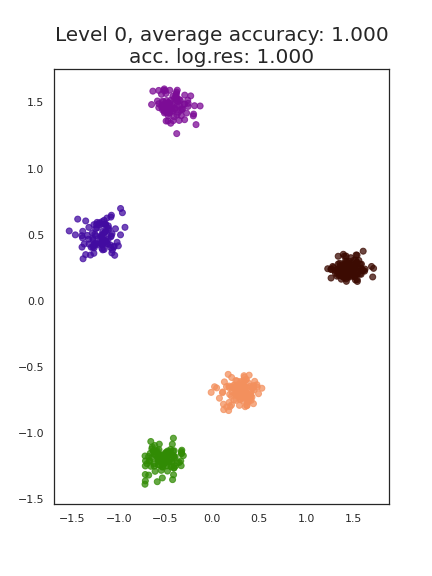
\includegraphics[width=.4\linewidth]{figs/simple_5_nuts.png}
    \caption[HmPPPCAs model performed on the simple Splatter data-set with 5 genes using NUTS]{\small \textbf{HmPPPCAs model performed on the simple Splatter data-set with 5 genes using NUTS.} The maximum accuracy of $1.0$ was found on the top-level. The clusters found within the top-level PPCA have been numbered. The colours indicate different cell types.}
    \label{fig:simple_5_nuts}
\end{figure}

\begin{figure}
    \centering
    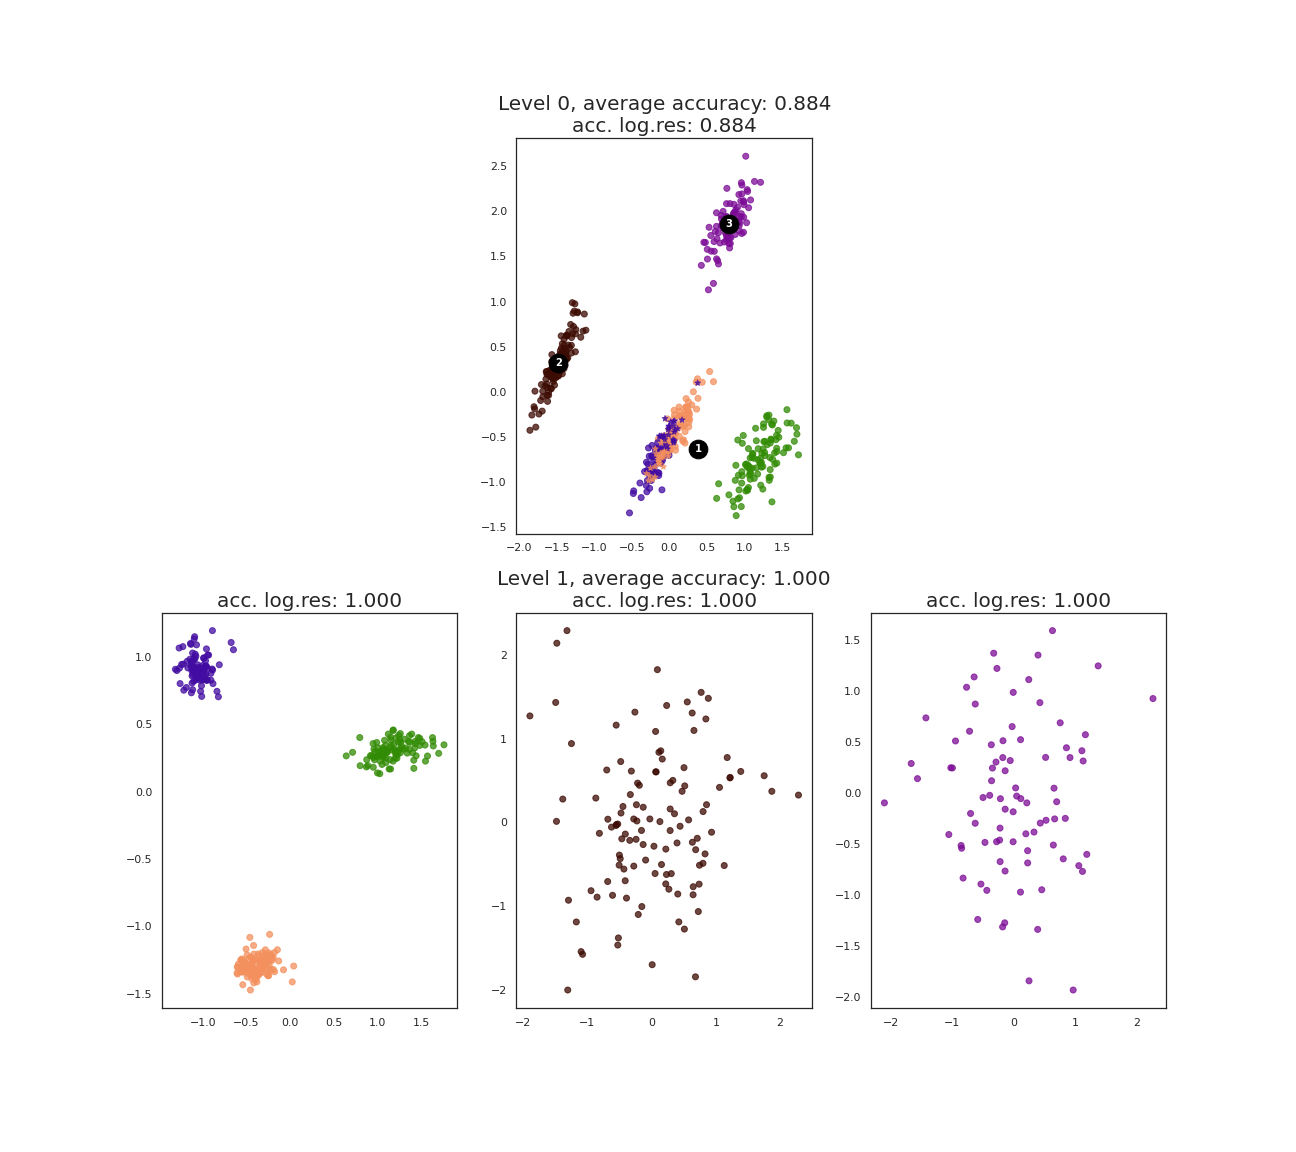
\includegraphics[width=\linewidth]{figs/simple_25_nuts.png}
    \caption[HmPPPCAs model performed on the simple Splatter data-set with 25 genes using NUTS]{\small \textbf{HmPPPCAs model performed on the simple Splatter data-set with 25 genes using NUTS.} \small The maximum accuracy of $1.0$ was found at level $1$. The top-level PPCA achieved an accuracy of $0.884$. The clusters found within the top-level PPCA have been numbered. The colours indicate different cell types. Data-points that were predicted correctly by the logistic regression are plotted with dots, incorrect predictions are plotted with stars.}
    \label{fig:simple_25_nuts}
\end{figure}

\begin{figure}
    \centering
    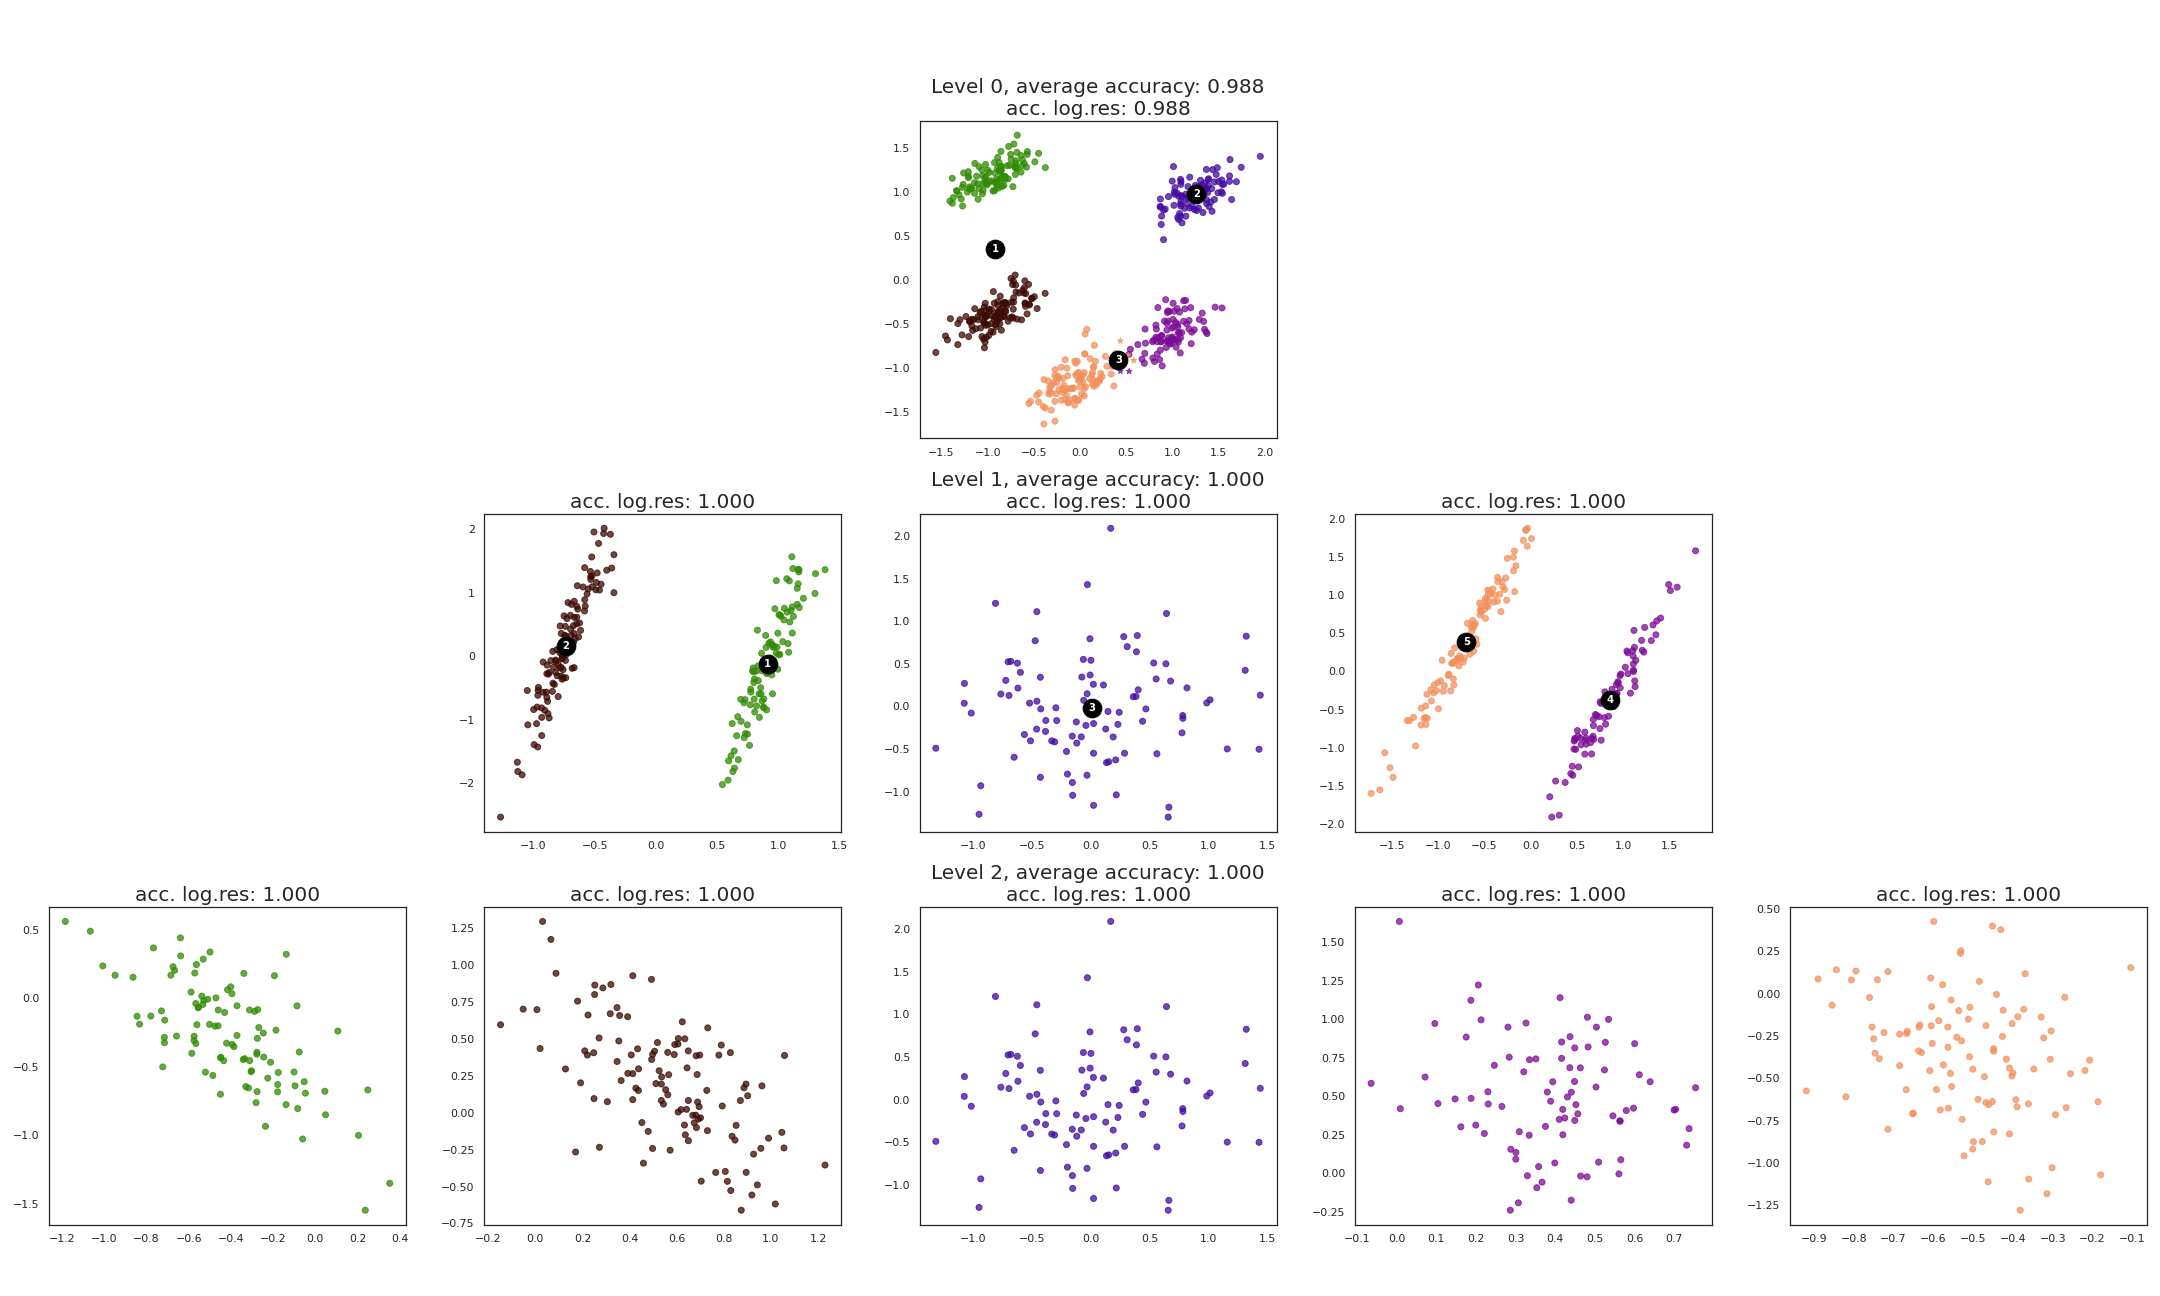
\includegraphics[width=\linewidth]{figs/simple_50_nuts.png}
    \caption[HmPPPCAs model performed on the simple Splatter data-set with 50 genes using NUTS]{\small \textbf{HmPPPCAs model performed on the simple Splatter data-set with 50 genes using NUTS.} \small The maximum accuracy of $1.0$ was found at level $1$. The top-level PPCA achieved an accuracy of $0.988$. The clusters found within the top-level PPCA have been numbered. The colours indicate different cell types. Data-points that were predicted correctly by the logistic regression are plotted with dots, incorrect predictions are plotted with stars.}
    \label{fig:simple_50_nuts}
\end{figure}

\begin{figure}
    \centering
    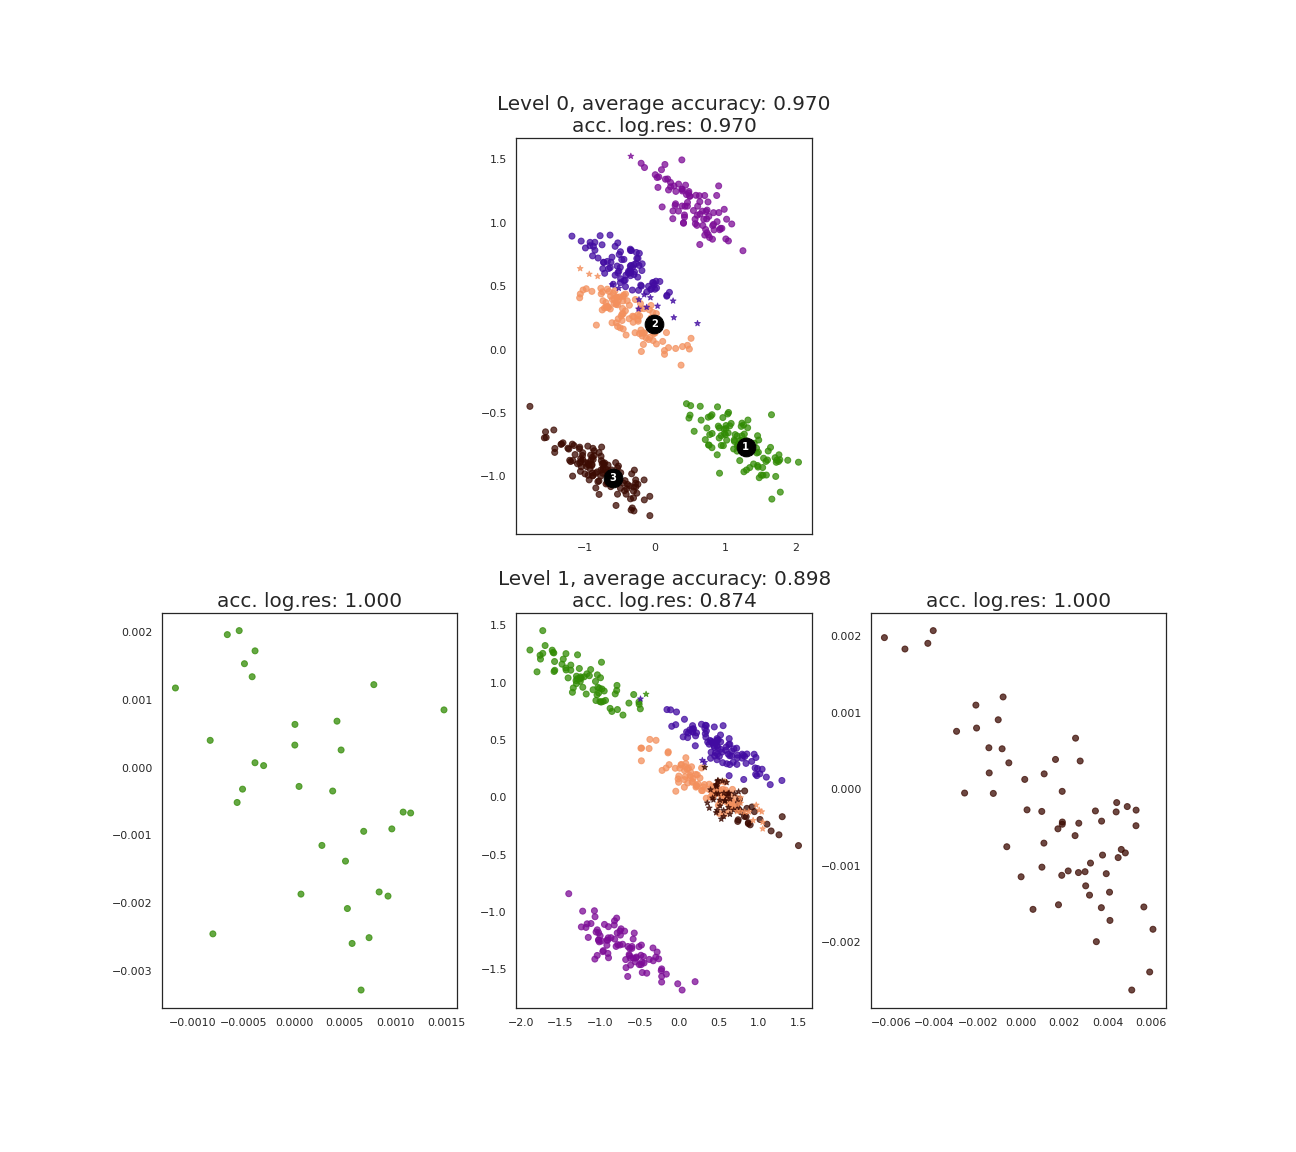
\includegraphics[width=\linewidth]{figs/simple_150_nuts.png}
    \caption[HmPPPCAs model performed on the simple Splatter data-set with 150 genes using NUTS]{\small \textbf{HmPPPCAs model performed on the simple Splatter data-set with 150 genes using NUTS.} \small The maximum accuracy of $0.970$ was found on the top-level. The clusters found within the top-level PPCA have been numbered. The colours indicate different cell types. Data-points that were predicted correctly by the logistic regression are plotted with dots, incorrect predictions are plotted with stars.}
    \label{fig:simple_150_nuts}
\end{figure}

\begin{figure}
    \centering
    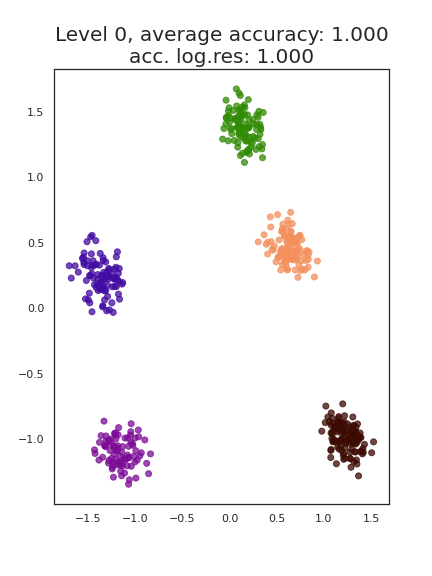
\includegraphics[width=.6\linewidth]{figs/simple_5_vb.png}
    \caption[HmPPPCAs model performed on the simple Splatter data-set with 5 genes using VB]{\small \textbf{HmPPPCAs model performed on the simple Splatter data-set with 5 genes using VB.} \small The maximum accuracy of $1.0$ was found on the top-level. The clusters found within the top-level PPCA have been numbered. The colours indicate different cell types.}
    \label{fig:simple_5_vb}
\end{figure}

\begin{figure}
    \centering
    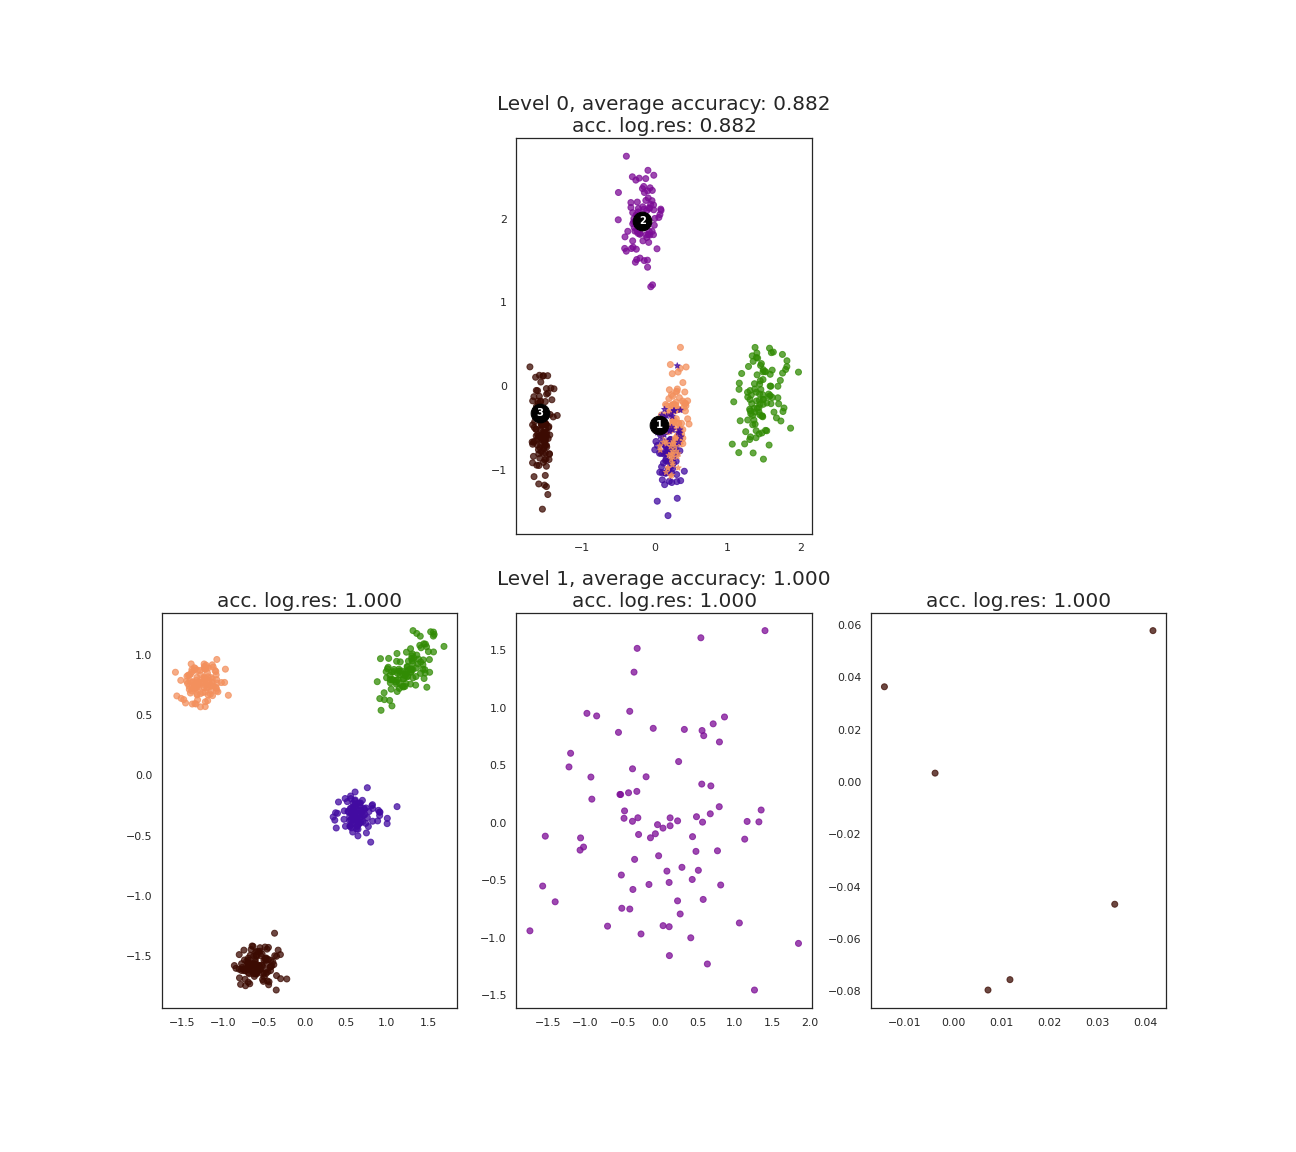
\includegraphics[width=\linewidth]{figs/simple_25_vb.png}
    \caption[HmPPPCAs model performed on the simple Splatter data-set with 25 genes using VB]{\small \textbf{HmPPPCAs model performed on the simple Splatter data-set with 25 genes using VB.} \small The maximum accuracy of $1.0$ was found at level $1$. The top-level PPCA achieved an accuracy of $0.882$. The clusters found within the top-level PPCA have been numbered. The colours indicate different cell types. Data-points that were predicted correctly by the logistic regression are plotted with dots, incorrect predictions are plotted with stars.}
    \label{fig:simple_25_vb}
\end{figure}

\begin{figure}
    \centering
    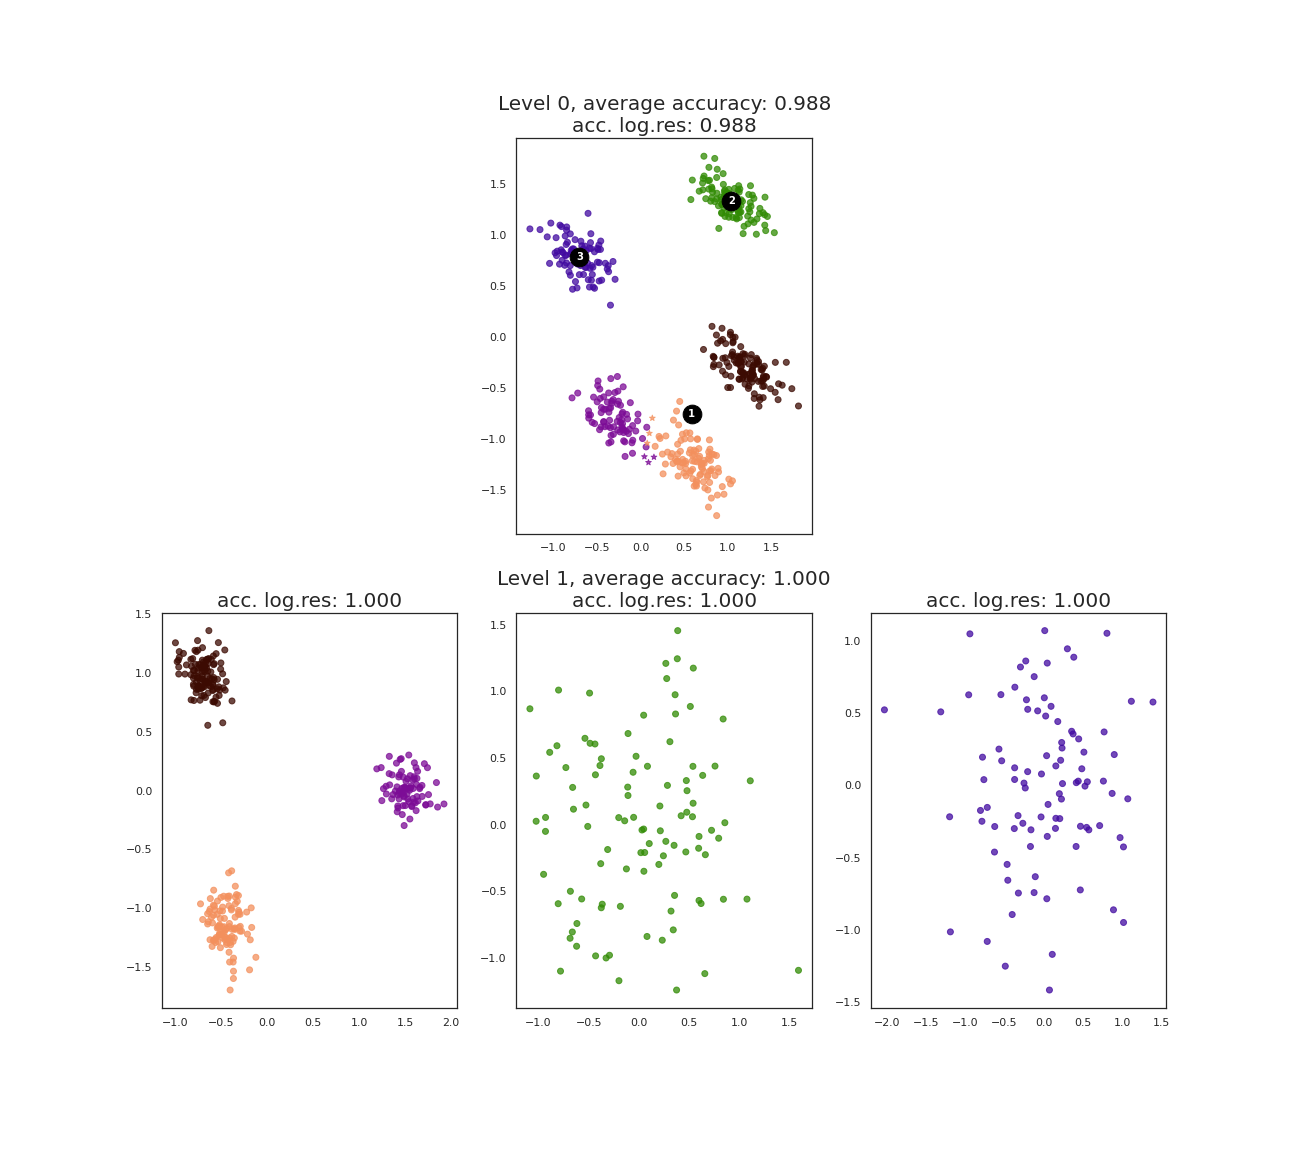
\includegraphics[width=\linewidth]{figs/simple_50_vb.png}
    \caption[HmPPPCAs model performed on the simple Splatter data-set with 50 genes using VB]{\small \textbf{HmPPPCAs model performed on the simple Splatter data-set with 50 genes using VB.} \small The maximum accuracy of $1.0$ was found at level $1$. The top-level PPCA achieved an accuracy of $0.988$. The clusters found within the top-level PPCA have been numbered. The colours indicate different cell types. Data-points that were predicted correctly by the logistic regression are plotted with dots, incorrect predictions are plotted with stars.}
    \label{fig:simple_50_vb}
\end{figure}

\begin{figure}
    \centering
    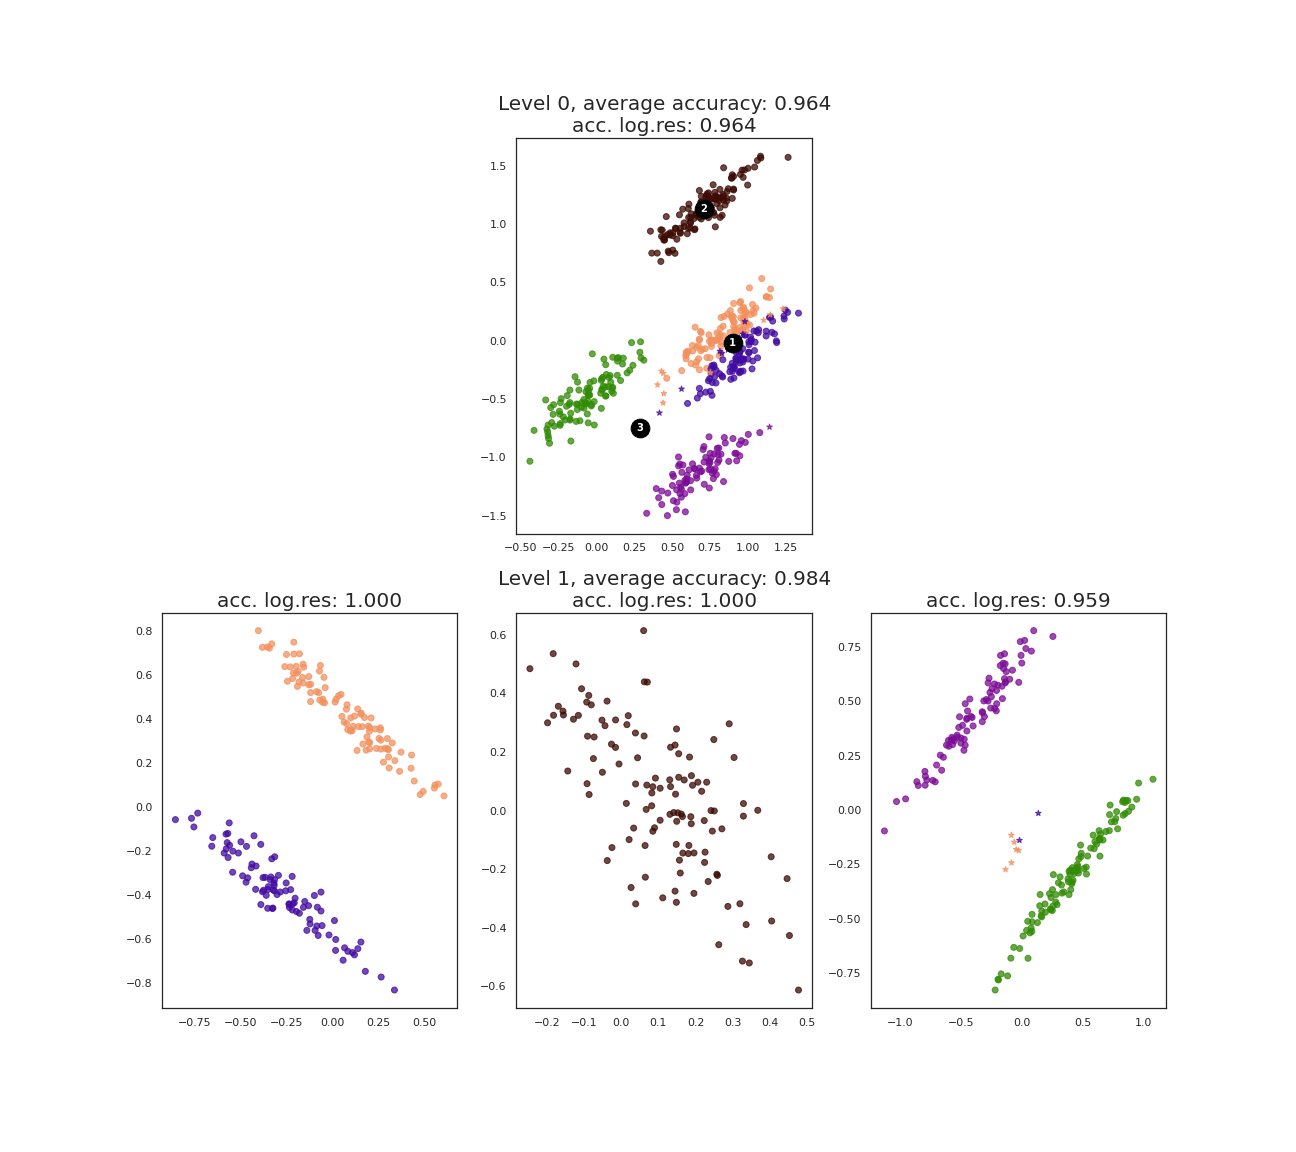
\includegraphics[width=\linewidth]{figs/simple_150_vb.png}
    \caption[HmPPPCAs model performed on the simple Splatter data-set with 150 genes using VB]{\small \textbf{HmPPPCAs model performed on the simple Splatter data-set with 150 genes using VB.} \small The maximum accuracy of $0.984$ was found at level $1$. The top-level PPCA achieved an accuracy of $0.964$. The clusters found within the top-level PPCA have been numbered. The colours indicate different cell types. Data-points that were predicted correctly by the logistic regression are plotted with dots, incorrect predictions are plotted with stars.}
    \label{fig:simple_150_vb}
\end{figure}

\clearpage
% \newpage

\section{Complex Splatter data-sets}\label{sec:complex}

\begin{figure}[h]
    \centering
    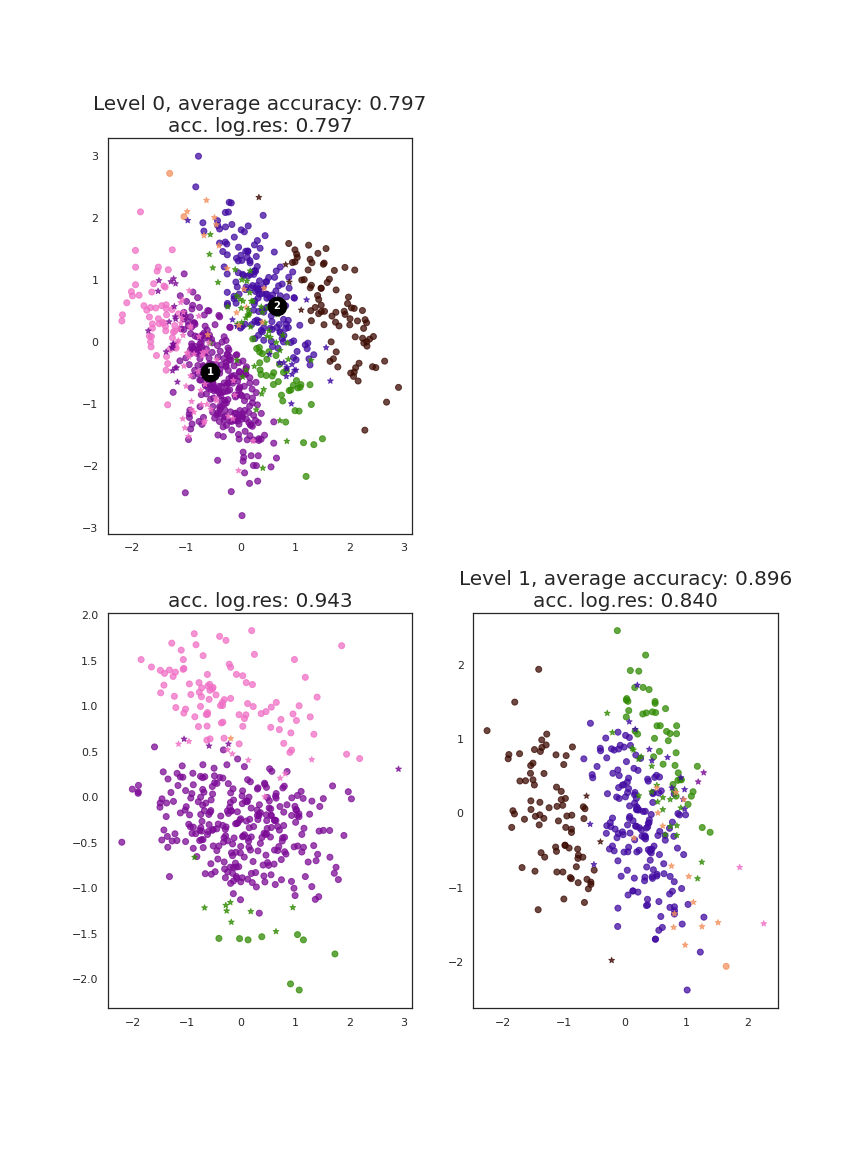
\includegraphics[width=.8\linewidth]{figs/complex_5_nuts.png}
    \caption[HmPPPCAs model performed on the complex Splatter data-set with 5 genes using NUTS]{\small \textbf{HmPPPCAs model performed on the complex Splatter data-set with 5 genes using NUTS.} \small The maximum accuracy of $0.896$ was found at level $1$. The top-level PPCA achieved an accuracy of $0.797$. The clusters found within the top-level PPCA have been numbered. The colours indicate different cell types. Data-points that were predicted correctly by the logistic regression are plotted with dots, incorrect predictions are plotted with stars.}
    \label{fig:complex_5_nuts}
\end{figure}

\begin{figure}
    \centering
    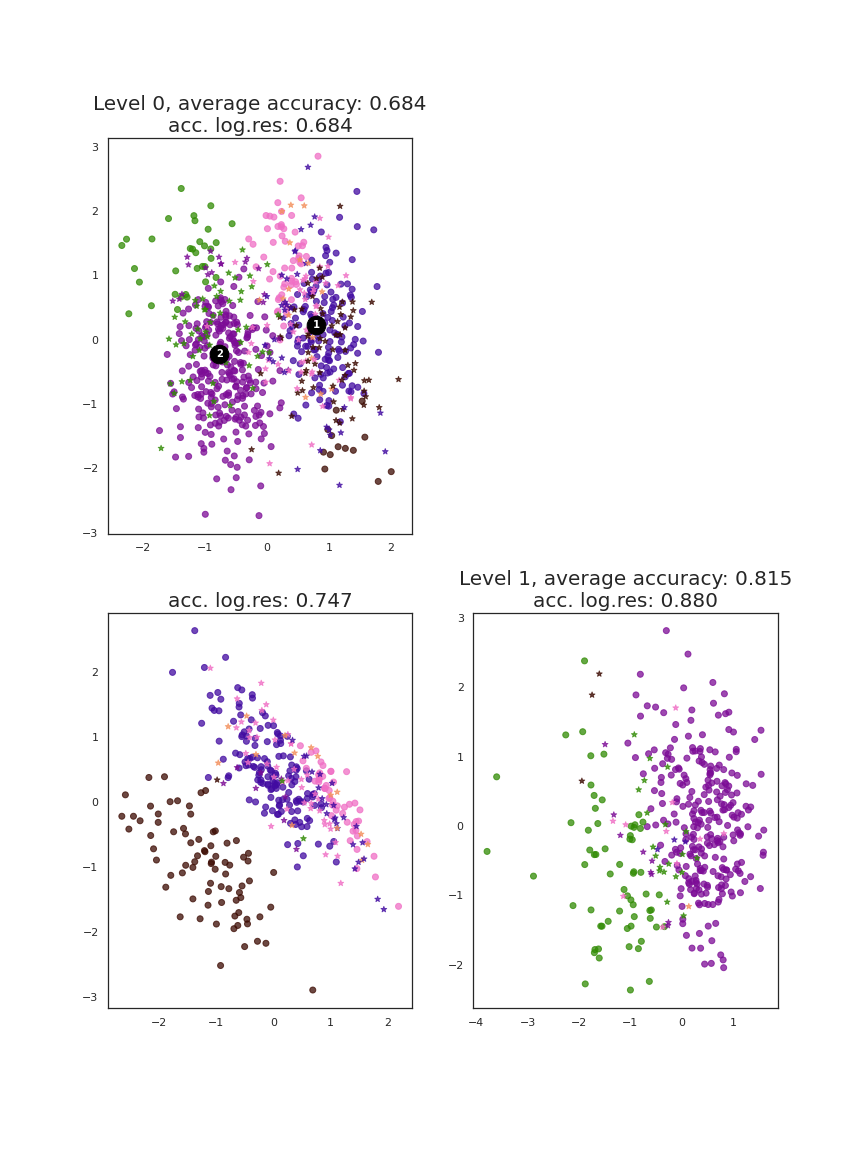
\includegraphics[width=\linewidth]{figs/complex_25_nuts.png}
    \caption[HmPPPCAs model performed on the complex Splatter data-set with 25 genes using NUTS]{\small \textbf{HmPPPCAs model performed on the complex Splatter data-set with 25 genes using NUTS.} \small The maximum accuracy of $0.815$ was found at level $1$. The top-level PPCA achieved an accuracy of $0.684$. The clusters found within the top-level PPCA have been numbered. The colours indicate different cell types. Data-points that were predicted correctly by the logistic regression are plotted with dots, incorrect predictions are plotted with stars.}
    \label{fig:complex_25_nuts}
\end{figure}

\begin{figure}
    \centering
    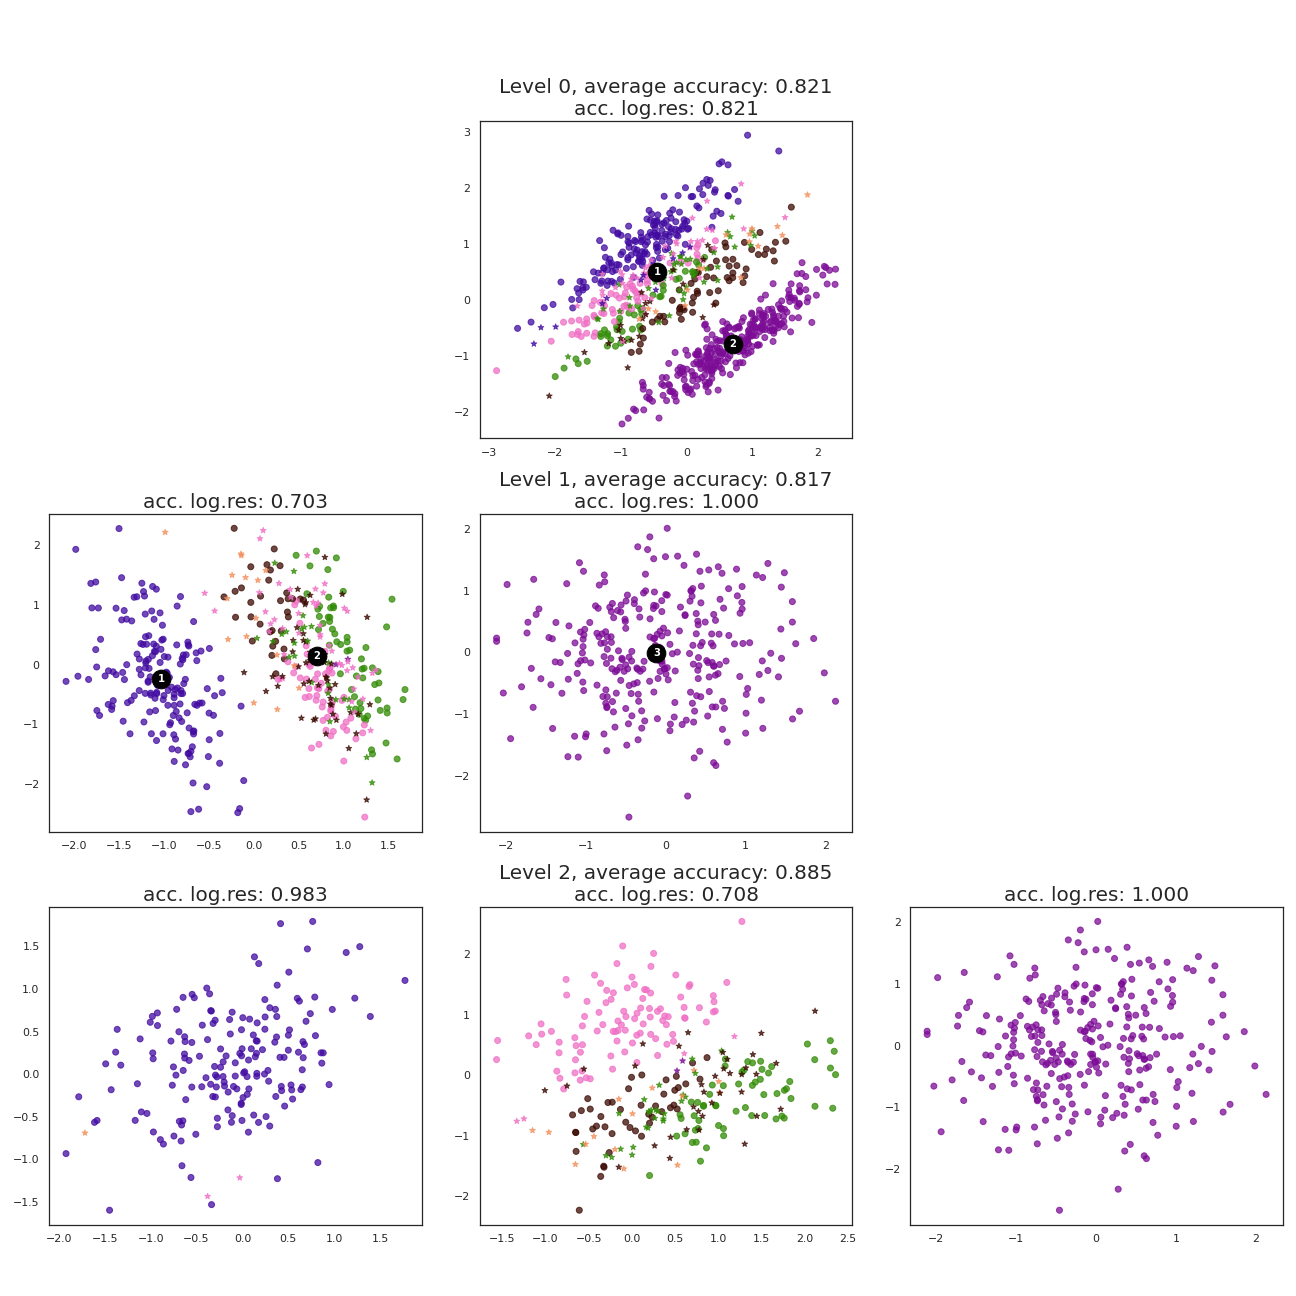
\includegraphics[width=\linewidth]{figs/complex_50_nuts.png}
    \caption[HmPPPCAs model performed on the complex Splatter data-set with 50 genes using NUTS]{\small \textbf{HmPPPCAs model performed on the complex Splatter data-set with 50 genes using NUTS.} \small The maximum accuracy of $0.885$ was found at level $2$. The top-level PPCA achieved an accuracy of $0.821$. The clusters found within each level have been numbered. The colours indicate different cell types. Data-points that were predicted correctly by the logistic regression are plotted with dots, incorrect predictions are plotted with stars.}
    \label{fig:complex_50_nuts}
\end{figure}

\begin{figure}
    \centering
    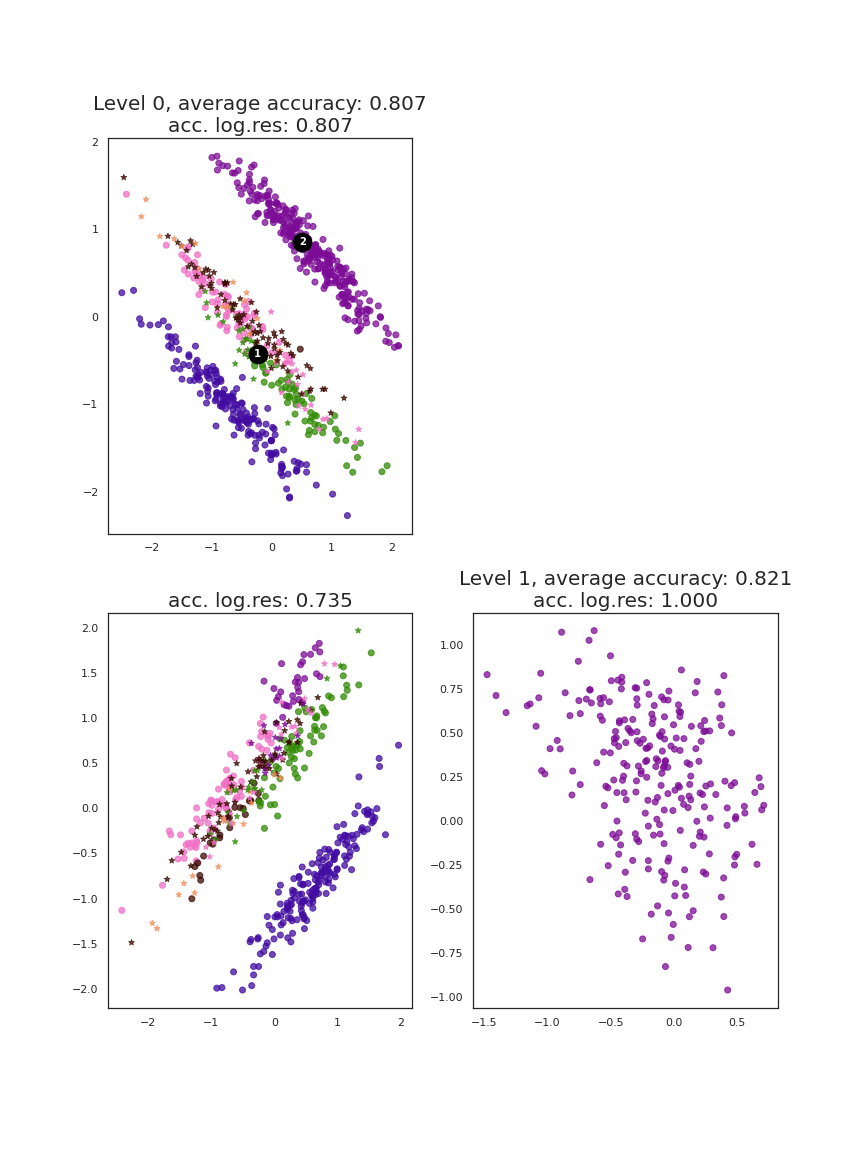
\includegraphics[width=\linewidth]{figs/complex_150_nuts.png}
    \caption[HmPPPCAs model performed on the complex Splatter data-set with 150 genes using NUTS]{\small \textbf{HmPPPCAs model performed on the complex Splatter data-set with 150 genes using NUTS.} \small The maximum accuracy of $0.821$ was found at level $1$. The top-level PPCA achieved an accuracy of $0.807$. The clusters found within the top-level PPCA have been numbered. The colours indicate different cell types. Data-points that were predicted correctly by the logistic regression are plotted with dots, incorrect predictions are plotted with stars.}
    \label{fig:complex_150_nuts}
\end{figure}



\begin{figure}
    \centering
    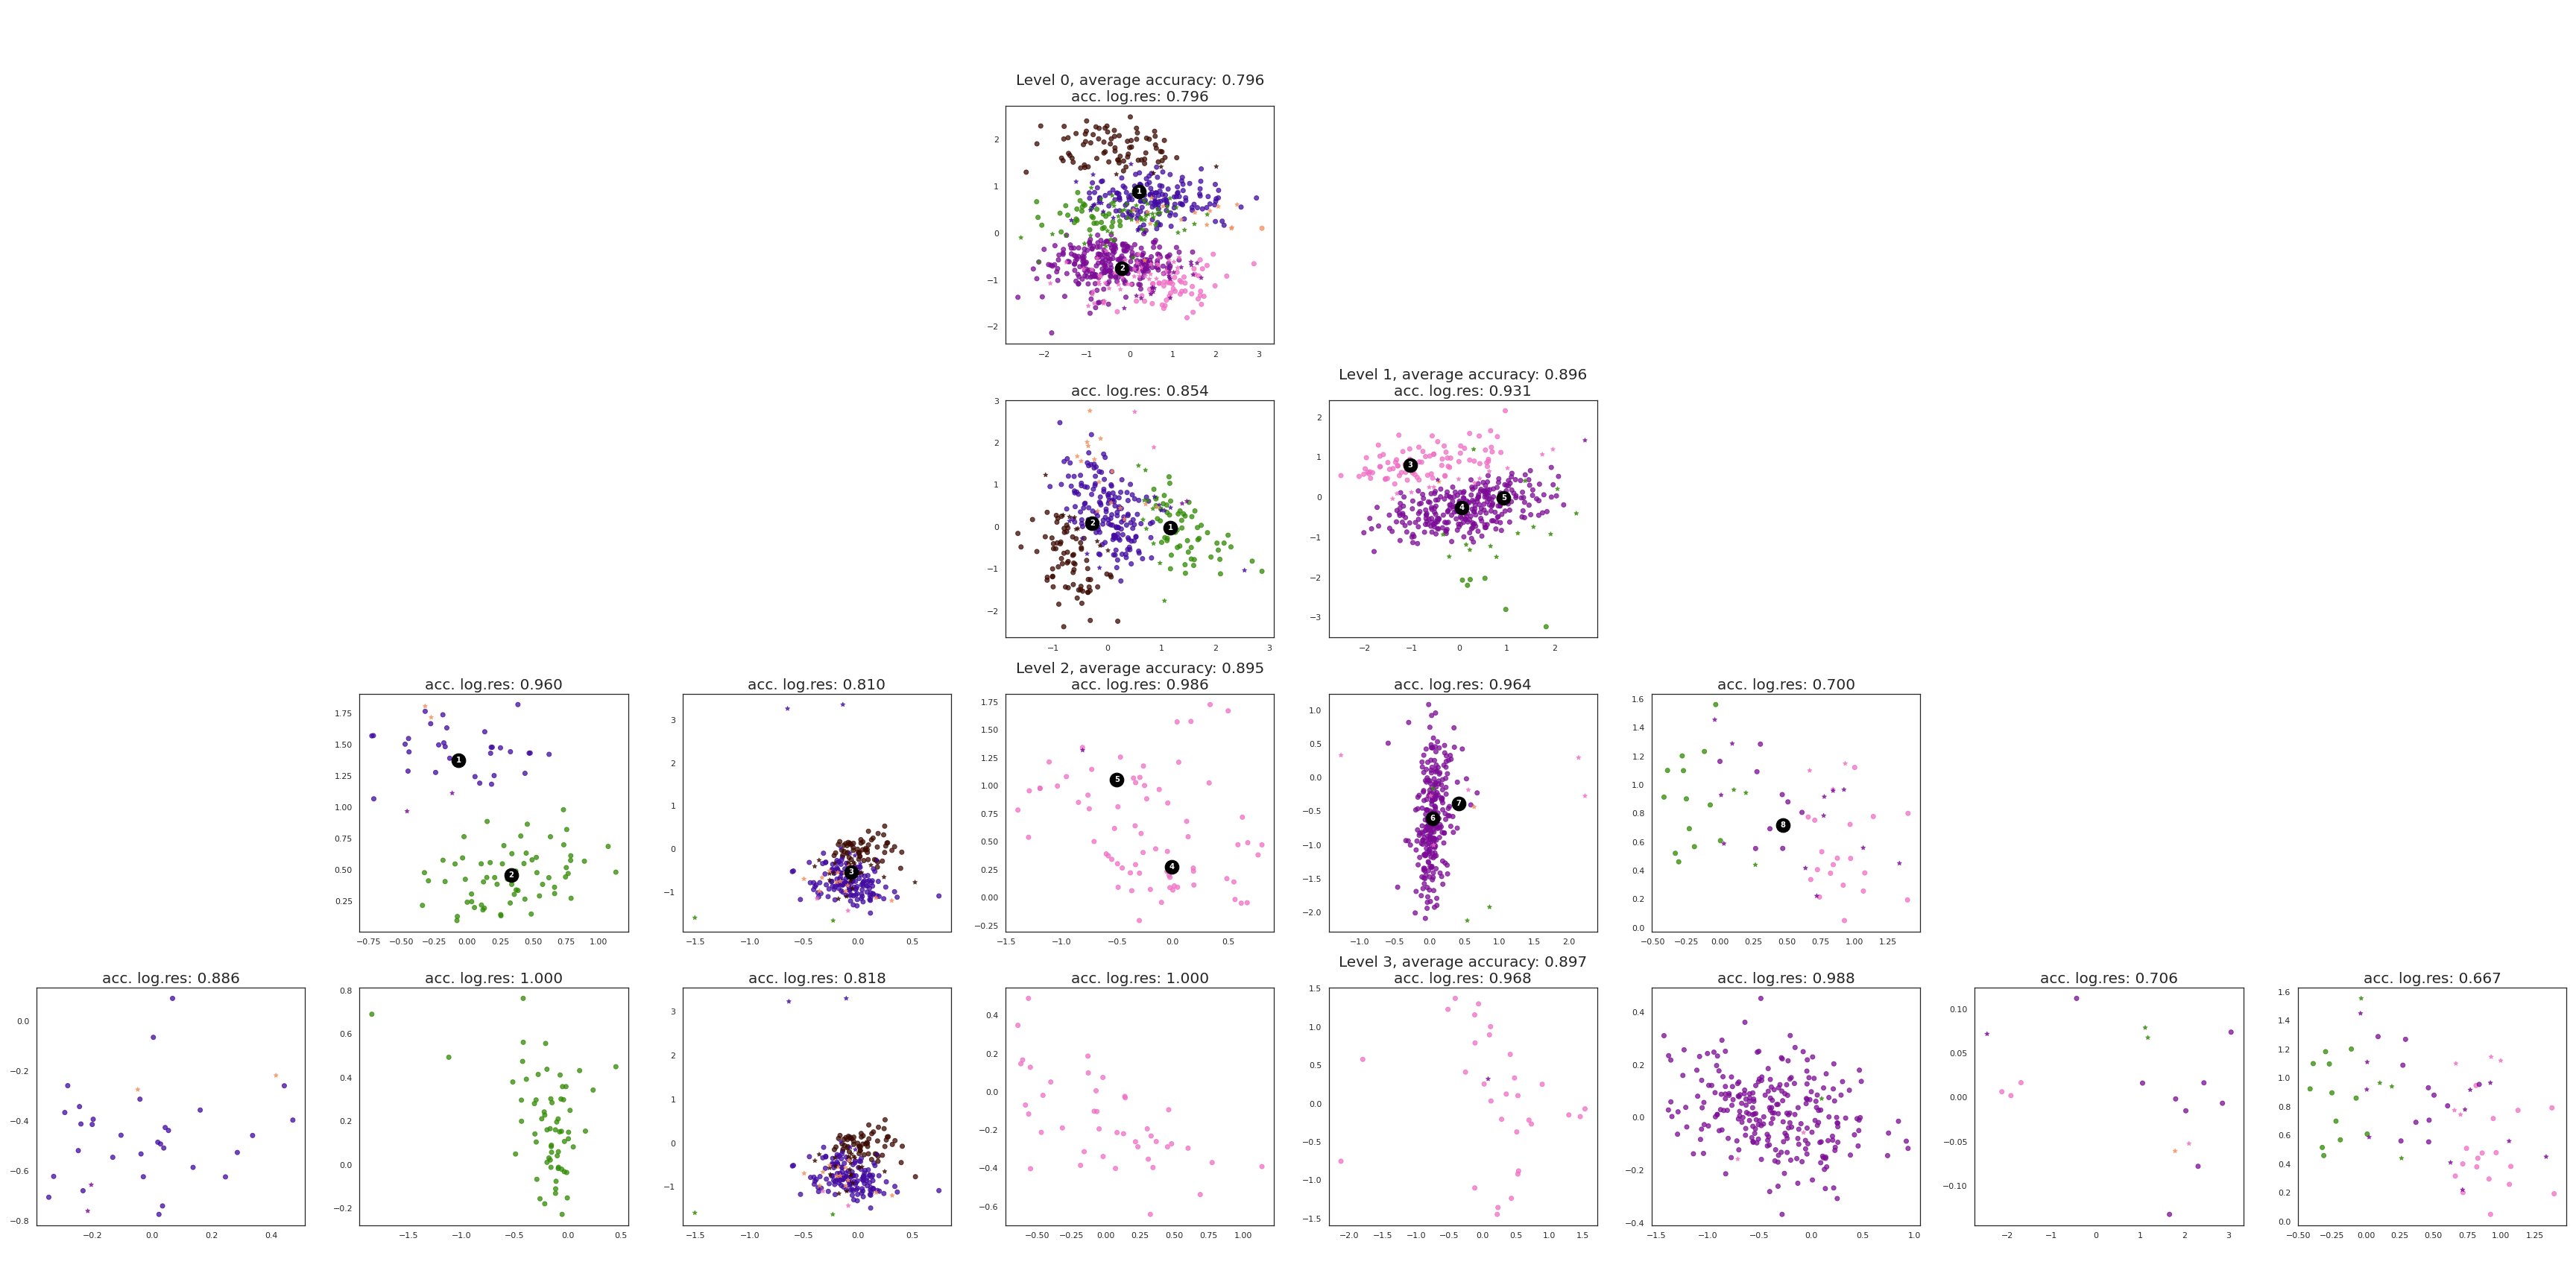
\includegraphics[width=\linewidth]{figs/complex_5_vb.png}
    \caption[HmPPPCAs model performed on the complex Splatter data-set with 5 genes using VB]{\small \textbf{HmPPPCAs model performed on the complex Splatter data-set with 5 genes using VB.} \small The maximum accuracy of $0.897$ was found at level $3$. The top-level PPCA achieved an accuracy of $0.796$. The clusters found within each level have been numbered. The colours indicate different cell types. Data-points that were predicted correctly by the logistic regression are plotted with dots, incorrect predictions are plotted with stars.}
    \label{fig:complex_5_vb}
\end{figure}

\begin{figure}
    \centering
    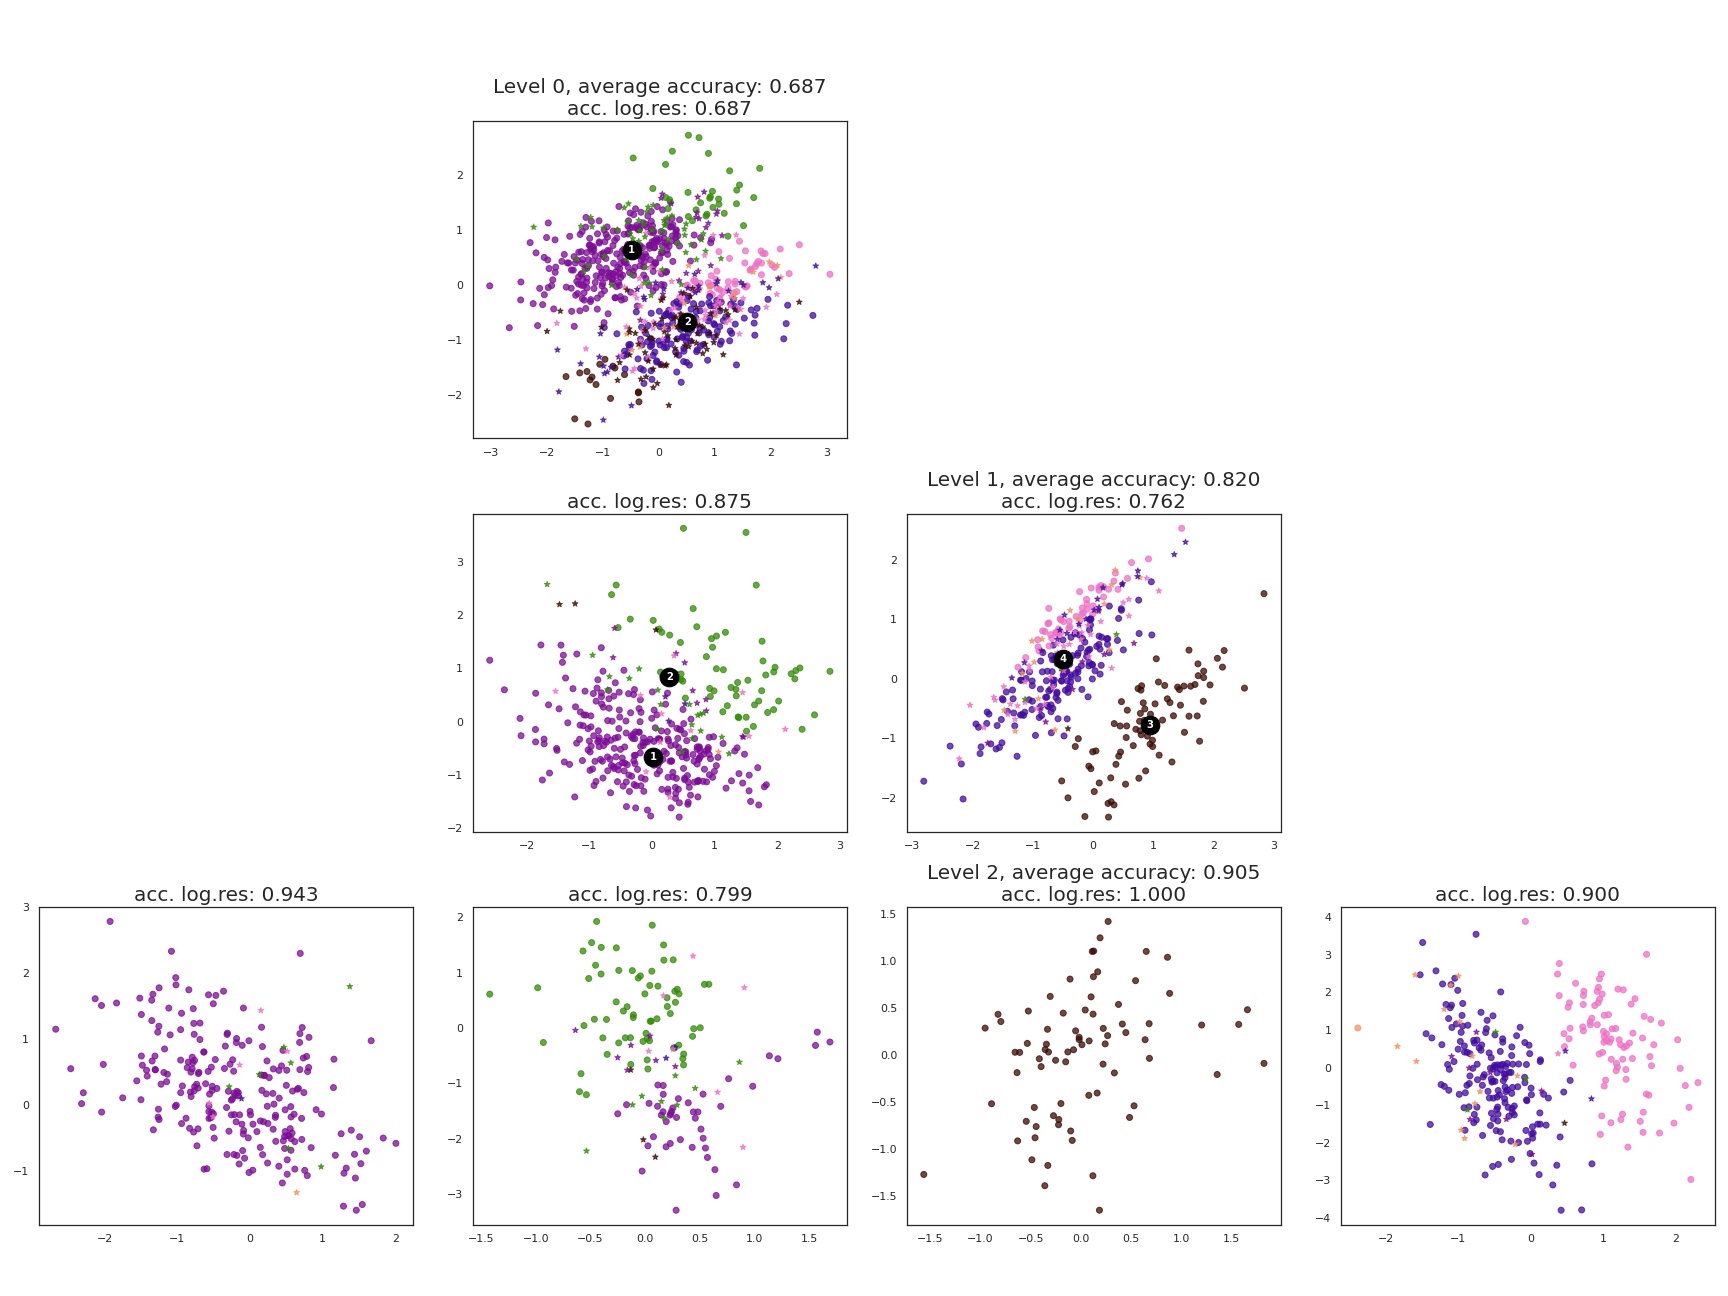
\includegraphics[width=\linewidth]{figs/complex_25_vb.png}
    \caption[HmPPPCAs model performed on the complex Splatter data-set with 25 genes using VB]{\small \textbf{HmPPPCAs model performed on the complex Splatter data-set with 25 genes using VB.} \small The maximum accuracy of $0.905$ was found at level $2$. The top-level PPCA achieved an accuracy of $0.687$. The clusters found within each level have been numbered. The colours indicate different cell types. Data-points that were predicted correctly by the logistic regression are plotted with dots, incorrect predictions are plotted with stars.}
    \label{fig:complex_25_vb}
\end{figure}

\begin{figure}
    \centering
    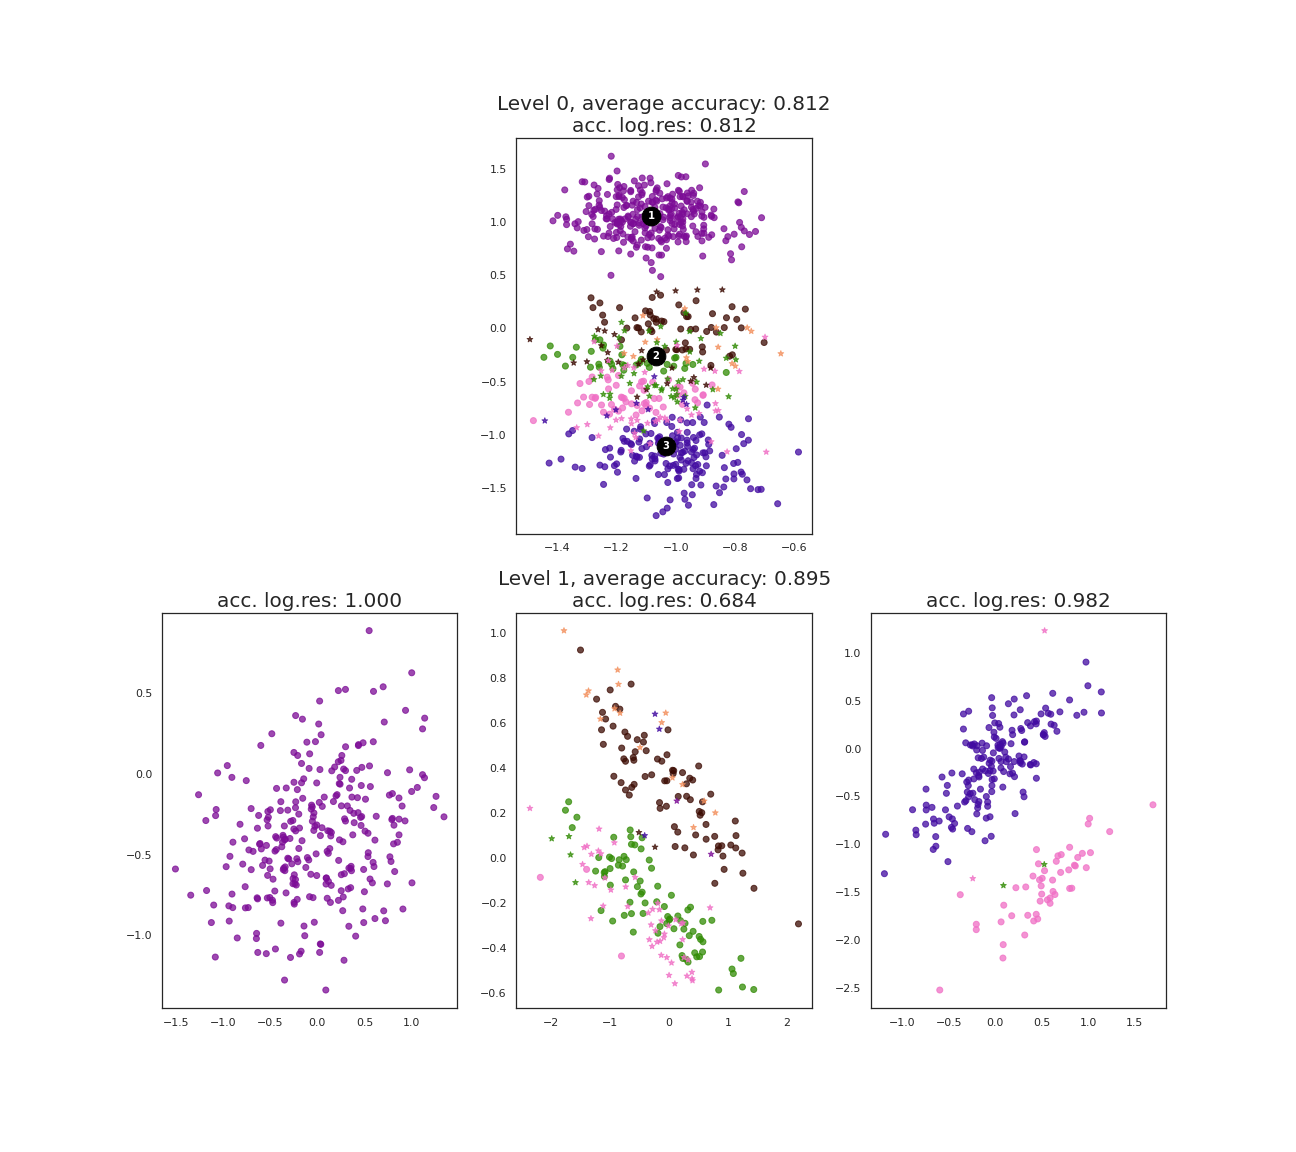
\includegraphics[width=\linewidth]{figs/complex_50_vb.png}
    \caption[HmPPPCAs model performed on the complex Splatter data-set with 50 genes using VB]{\small \textbf{HmPPPCAs model performed on the complex Splatter data-set with 50 genes using VB.} \small The maximum accuracy of $0.895$ was found at level $1$. The top-level PPCA achieved an accuracy of $0.812$. The clusters found within the top-level PPCA have been numbered. The colours indicate different cell types. Data-points that were predicted correctly by the logistic regression are plotted with dots, incorrect predictions are plotted with stars.}
    \label{fig:complex_50_vb}
\end{figure}

\begin{figure}
    \centering
    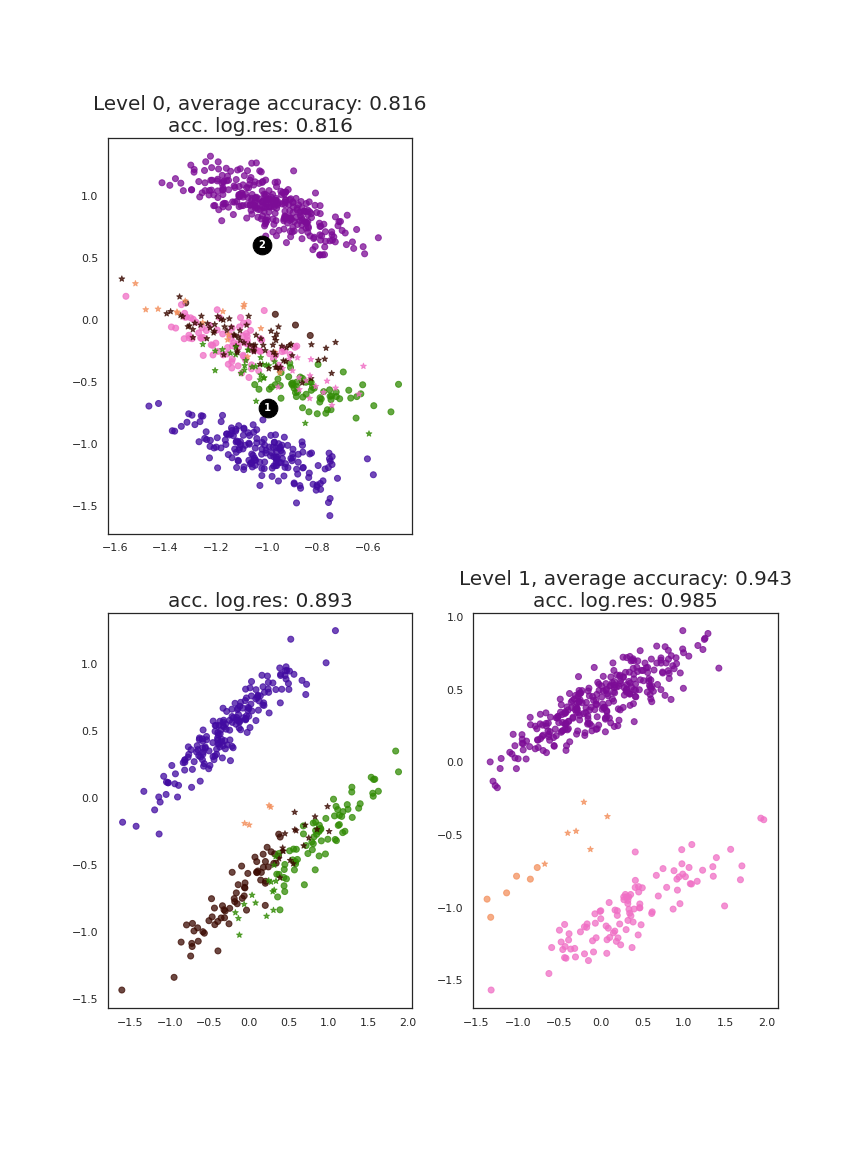
\includegraphics[width=\linewidth]{figs/complex_150_vb.png}
    \caption[HmPPPCAs model performed on the complex Splatter data-set with 150 genes using VB]{\small \textbf{HmPPPCAs model performed on the complex Splatter data-set with 150 genes using VB.} \small The maximum accuracy of $0.943$ was found at level $1$. The top-level PPCA achieved an accuracy of $0.816$. The clusters found within the top-level PPCA have been numbered. The colours indicate different cell types. Data-points that were predicted correctly by the logistic regression are plotted with dots, incorrect predictions are plotted with stars.}
    \label{fig:complex_150_vb}
\end{figure}

\clearpage
% \newpage

\section{UMAP and t-SNE results on the Splatter data-sets}\label{sec:baselineresults}


\begin{figure}[h]
\centering
\begin{subfigure}{.3\textwidth}
  \centering
  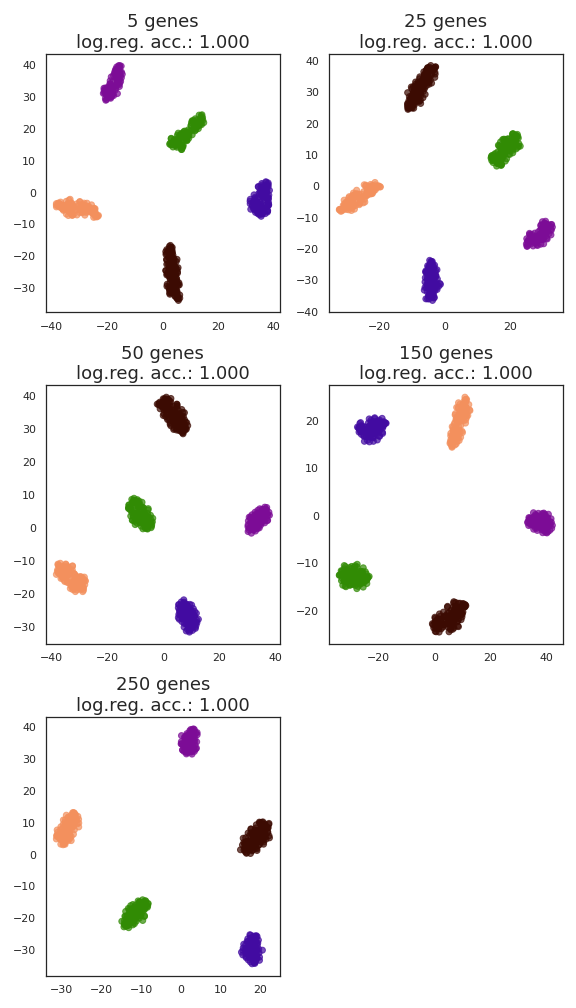
\includegraphics[width=\linewidth]{figs/TSNE_simple.png}
  \caption{\small t-SNE performance on the simple Splatter data-sets}
  \label{fig:tmse_simple}
\end{subfigure}\hspace{30px}%
\begin{subfigure}{.3\textwidth}
  \centering
  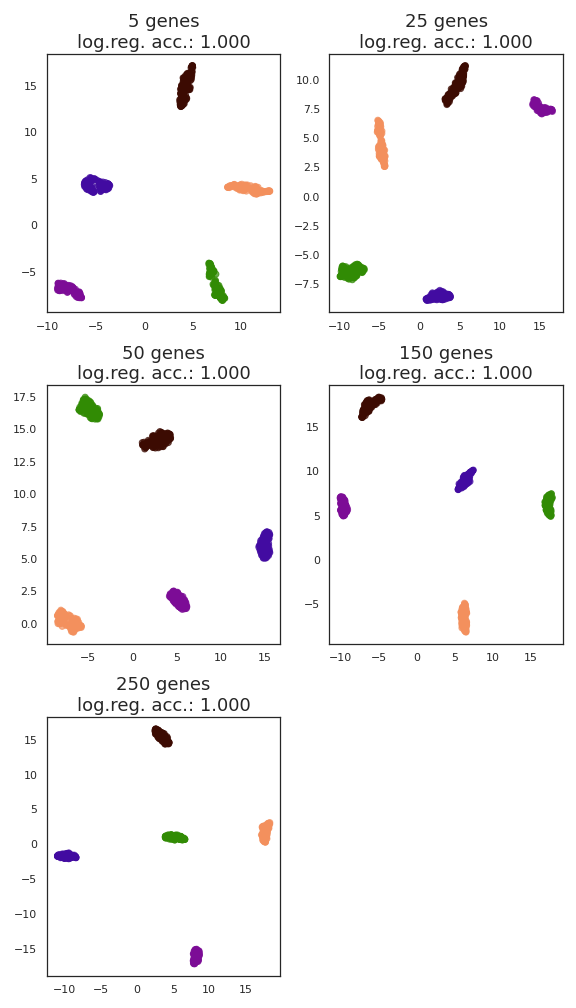
\includegraphics[width=\linewidth]{figs/UMAP_simple.png}
  \caption{\small UMAP performance on the simple Splatter data-sets}
  \label{fig:umap_simple}
\end{subfigure}
% \small
% \caption[t-SNE (left) and UMAP (right) performance on the simple Splatter data-sets.]{\small \textbf{t-SNE (left) and UMAP (right) performance on the simple Splatter data-sets.} \small
% In both figures, the plot with colours based on the original labels is given on the left, with the logistic regression predictions given on the right.}

\begin{subfigure}{.3\textwidth}
  \centering
  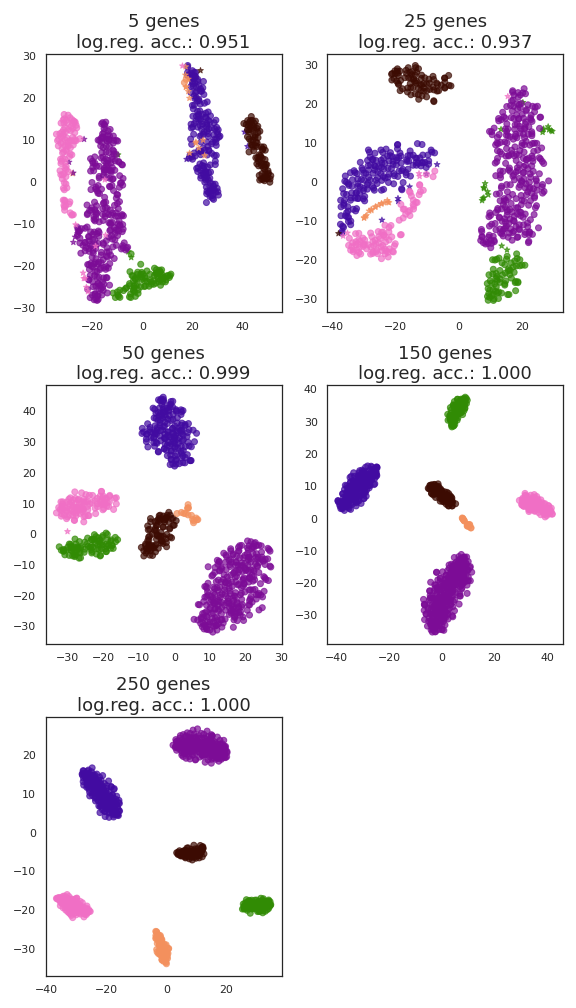
\includegraphics[width=\linewidth]{figs/TSNE_complex.png}
  \caption{\small t-SNE performance on the complex Splatter data-sets}
  \label{fig:tsne_complex}
\end{subfigure}\hspace{30px}%
\begin{subfigure}{.3\textwidth}
  \centering
  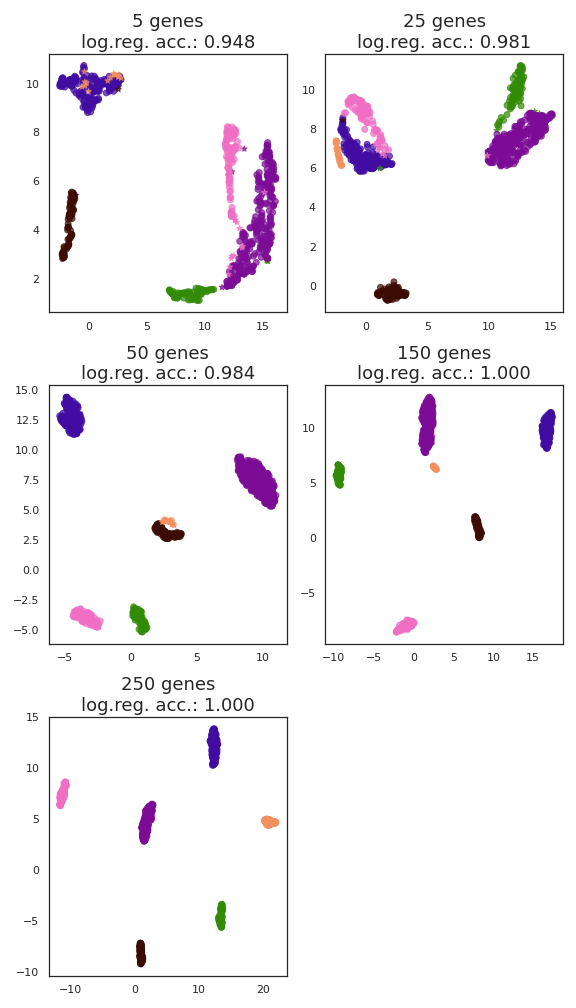
\includegraphics[width=\linewidth]{figs/UMAP_complex.png}
  \caption{\small UMAP performance on the complex Splatter data-sets}
  \label{fig:umap_complex}
\end{subfigure}
\small
\caption[t-SNE and UMAP performance on the Splatter data-sets.]{\small \textbf{t-SNE and UMAP performance on the Splatter data-sets.} \small The resulting plots when analyzing the simple Splatter data-sets with t-SNE (a) and UMAP (b) and when analyzing the complex Splatter data-sets with t-SNE (c) and UMAP (d). Colours indicate different cell types. Data-points that were predicted correctly by the logistic regression are plotted with dots, incorrect predictions are plotted with stars.}
\label{fig:baseline_splatter}
\end{figure}



\begin{figure}
    \centering
    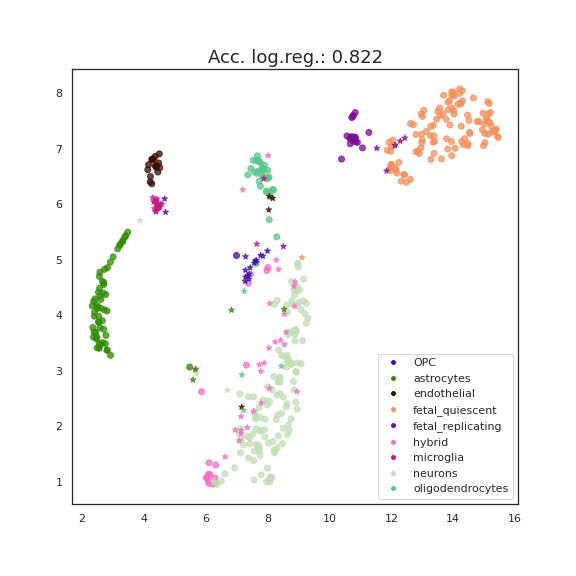
\includegraphics[width=.6\linewidth]{figs/darmanis_UMAP_logres.png}
    \caption[UMAP results of the Darmanis data-set.]{\small \textbf{UMAP results of the Darmanis data-set.} \small An accuracy of $0.822$ was measured after performing a logistic regression with a 5-fold cross validation. Colours indicate different cell types. Data-points that were predicted correctly by the logistic regression are plotted with dots, incorrect predictions are plotted with stars.}
    \label{fig:darmanis_umap}
\end{figure}

\begin{figure}
    \centering
    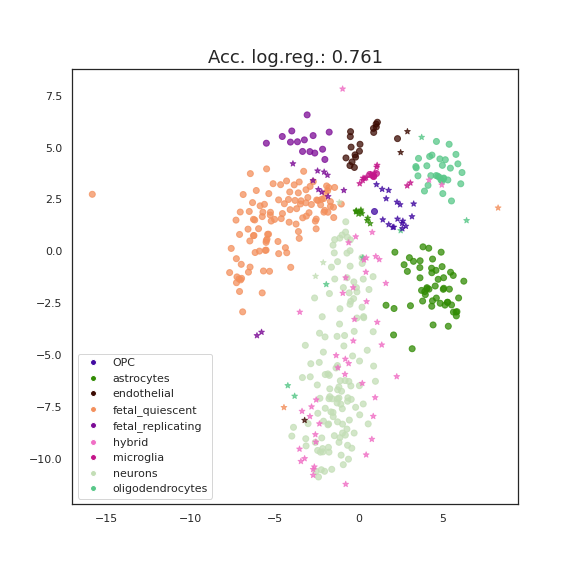
\includegraphics[width=.6\linewidth]{figs/darmanis_tsne_logres.png}
    \caption[t-SNE results of the Darmanis data-set.]{\small \textbf{t-SNE results of the Darmanis data-set.} \small An accuracy of $0.761$ was measured after performing a logistic regression with a 5-fold cross validation. Colours indicate different cell types. Data-points that were predicted correctly by the logistic regression are plotted with dots, incorrect predictions are plotted with stars.}
    \label{fig:darmanis_tsne}
\end{figure}



\begin{figure}
    \centering
    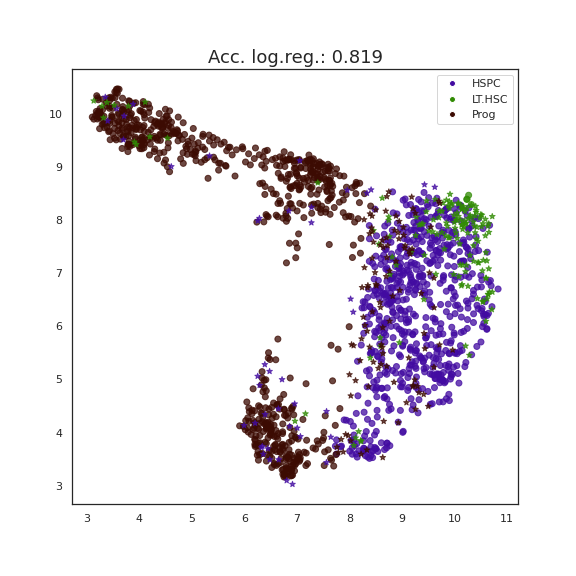
\includegraphics[width=.6\linewidth]{figs/nestorowa_UMAP_logres.png}
    \caption[UMAP results of the Nestorowa data-set.]{\small \textbf{UMAP results of the Nestorowa data-set.} \small An accuracy of $0.819$ was measured after performing a logistic regression with a 5-fold cross validation. Colours indicate different cell types. Data-points that were predicted correctly by the logistic regression are plotted with dots, incorrect predictions are plotted with stars.}
    \label{fig:nestorowa_umap}
\end{figure}

\begin{figure}
    \centering
    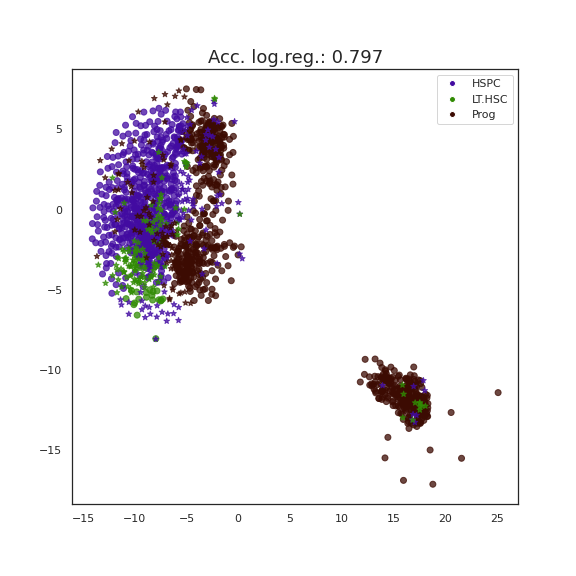
\includegraphics[width=.6\linewidth]{figs/nestorowa_tsne_logres.png}
    \caption[t-SNE results of the Nestorowa data-set.]{\small \textbf{t-SNE results of the Nestorowa data-set.} \small An accuracy of $0.797$ was measured after performing a logistic regression with a 5-fold cross validation. Colours indicate different cell types. Data-points that were predicted correctly by the logistic regression are plotted with dots, incorrect predictions are plotted with stars.}
    \label{fig:nestorowa_tsne}
\end{figure}


\addtocontents{toc}{\vspace{2em}} % Add a gap in the Contents, for aesthetics

\backmatter

%----------------------------------------------------------------------------------------
%	BIBLIOGRAPHY
%----------------------------------------------------------------------------------------

\label{References}

\lhead{\emph{References}} % Change the page header to say "Bibliography"

\bibliographystyle{unsrtnat} % Use the "unsrtnat" BibTeX style for formatting the Bibliography

\bibliography{refs} % The references (bibliography) information are stored in the file named "Bibliography.bib"




\end{document}  